\documentclass[a4paper,11pt,titlepage,oneside]{book}	%classe e struttura
\usepackage[english]{babel} 	%lingua principale
\usepackage[utf8]{inputenc}	%caratteri accentati
\usepackage{graphicx}		%pacchetto per le immagini
\usepackage{mathrsfs}		%pacchetto per scrittura manoscritto
\usepackage{booktabs}		%pacchetto per separatori tabelle
\usepackage{multirow}		%pacchetto per multirighe in tabelle
\usepackage{siunitx}		%pacchetto per le tabelle dati
\usepackage{wrapfig}		%pacchetto per le immagini immerse nel testo
\usepackage{latexsym}		%pacchetto per lettere greche
\usepackage{tabularx}		%pacchetto per tabelle 
\usepackage{amsmath}		%pacchetto per matematica
\usepackage{physics}		%pacchetto per fisica bra ket
\usepackage{subfig}		%pacchetto per sottotitoli a immagini
\usepackage{tikz}		%pacchetto per disegni
%\usepackage{circuitikz}	%pacchetto per disegni di circuiti
\usepackage{fancyhdr}
\usepackage{gensymb}
\usepackage{url}
\usepackage{hyperref}
\hypersetup{
	colorlinks,
	citecolor=black,
	filecolor=black,
	linkcolor=black,
	urlcolor=blue
}

\usepackage{frontespizio}

\frenchspacing 		%regola spazi
\raggedbottom		%spazio vuoto a fine pagina, quando finisce il testo, se lo togli allunga gli spazi per riempire nell'altezza la pagina

\begin{document}
	
	%---------FRONTESPIZIO-----
	\begin{frontespizio}
		\Universita{Pavia}
		\Logo[3cm]{logo}
		\Facolta{scienze matematiche, fisiche, naturali}
		\Corso[laurea]{Scienze Fisiche}
		\Annoaccademico{2019-2020}
		%\Titoletto{Tesi di laurea magistrale}
		\Titolo{IDEA Dual-Readout calorimeter:\\Full simulation chain and neural network on particle ID}
		\Punteggiatura{}
		\Candidato[462495]{Alessandro Villa}
		\NRelatore{Supervisore}{Supervisori}
		\Relatore{Dott. Roberto Ferrari}
		\NCorrelatore{Co-Supervisore}{Co-Supervisori}
		\Correlatore{Dott. Lorenzo Pezzotti}
	\end{frontespizio}
	
	%_________________________CORPO INIZIALE
	\begin{frontmatter}
		\tableofcontents
		
		%---------INTRODUZIONE------
		\chapter{Introduction}
The discovery of the Higgs boson in 2012 at CERN has opened the door for several new studies in particle physics.
%Its relatively small mass allows to produce it in high luminosity electron-positron colliders.
The Higgs boson plays a crucial role in the biggest mysteries of modern particle physics and the precise measurement of its properties, together with the properties of the $W$ and $Z$ bosons, will provide deep information about the Standard Model (SM) and the physics Beyond it (BSM). At present, several projects are ongoing to design the next big-collider and its detectors with the primary task of measuring the Higgs properties.\\

In the first chapter, a short introduction to the main goals of modern particle physics is presented. The current design of possible future electroweak collider facilities is described, pointing out their capabilities to improve our knowledge of the field.
Finally, the IDEA detector concept is outlined, being one of the multi-purpose detector concepts at future electroweak colliders.\\

The second chapter provides a theoretical background on calorimetry, starting from the interaction between particles and matter and the particle showering mechanism. A description of modern calorimeters is also provided, distinguishing between electromagnetic and hadronic calorimeters. Eventually, the dual-readout compensation technique, cornerstone of the IDEA calorimeter, is introduced.\\

The third chapter is dedicated to the Silicon PhotoMultipliers. They are the photodetectors envisaged to be coupled to the IDEA dual-readout calorimeter. Their working principle is described, followed by their characteristic features such as gain, photon detection efficiency, linearity and noise sources.\\

The fourth chapter describes the simulation chain of the IDEA dual-readout calorimeter combining the Monte Carlo simulation of the calorimeter with the readout system simulation, emulating the SiPM response. Several analyses were performed to evaluate the performance and validate the full simulation model. They are described here for the first time.\\

The last chapter introduces the application of deep learning algorithms to the IDEA calorimeter simulated data. Two different algorithms have been used to perform the very challenging task of discriminating between neutral pions and photons. Indeed, the high spatial resolution of the IDEA calorimeter allows to reconstruct the two-dimensional pattern of particle showers with great accuracy, thus providing a powerful input for neural-network applications. Encouraging results were found and are extensively reported in the thesis.\\
		
	\end{frontmatter}
	
	%_________________________CORPO CENTRALE
	\begin{mainmatter}
		%---------CAPITOLO 1--------
		\chapter{Future colliders}
The chapter begins with a short description of the most important goals in today's particle physics, starting from the possibilities opened by the discovery of the Higgs boson.\\
It continues with an overview on the different projects among high-energy $e^+e^-$ colliders, both circular and linear (also known as ``electroweak factories").\\
Eventually, the IDEA Detector concept is described as a general-purpose detector designed for future $e^+e^-$ circular colliders.

\section{Physics goals}
With the discovery of the Higgs boson ($H$) in 2012 by the ATLAS and CMS Collaborations \cite{ATLAS_H, CMS_H}, a new era has been opened where the new boson is not only a research object but also a tool for new particle physics studies.\\

Thanks to the relatively small mass, $\simeq 125$ GeV, the Higgs boson production is within the reach of high-luminosity future circular colliders. Their main production mechanism is the so-called Higgs-strahlung process, in which the Higgs recoils over a $Z$-boson produced at $E_{cm}\simeq 240$ GeV ($e^+ e^- \rightarrow Z H$).
In $HZ$ events, the recoil mass (defined as the invariant mass of the system recoiling against the Z boson) peaks at the Higgs mass, thus allowing to tag the events independently of the $H$ decay mode.
This process allows to measure the Higgs production cross section in a model-independent way. The other couplings are eventually extracted through branching-ratio and width measurements with a subpercent precision.

%The total Higgs production cross section can be measured in the Higgstrahlung process  looking at its presence as the recoil to the $Z$. In this way the $H$ boson is directly coupled to the $Z$ measurement.
%The $H Z$ events have their recoil mass equal to $m_H$, hence Higgs bosons can be counted from the accumulation around the $H$ mass value, allowing to determine the $H Z$ cross section ($\sigma_{HZ}$).
%In particular, the total cross section could be determined independently of the $H$ decay, by counting the Higgsstrahlung events characterised by a leptonic decay: $Z \rightarrow l^+ l^-$.
%This method disentangled the $H$ production from its decay, providing a model-independent determination of its total width and its other couplings through branching ratio measurements with a sub-percent precision.\\

The $H$ couplings to the first Standard Model family particles (i.e. electron, quark up and quark down), because of their small masses and related decay branching ratios, will not be directly measurable at these colliders. 
However, with beam energies $\simeq 125.09$ GeV, corresponding to the $H$ pole mass, leptonic colliders can contribute to set upper limits to the electron Yukawa coupling by taking advantage from the resonant $H$ production.
Also the $t$ Yukawa coupling and the $H$ self-coupling will not be directly measurable because their masses are too large for a kinematically open decay.
However, the CERN future electron-positron circular collider (FCC-ee), operating at $\sqrt{s} = 350$ GeV, could measure the $t$ Yukawa coupling with a precision of $10\%$ thanks to higher order corrections of processes at the $t\Bar{t}$ threshold.\\

%It is possible to predict mass and properties of the top-quark and of the bosons $Z$, $W$ and $H$ using the Standard Model. This predictions are obtained from precise measurements in the Electroweak sector and theoretical calculations.
%Quantities called Electroweak Precision Observables (EWPOs) can establish the presence of new physics. For this reason EWPOs measurements represent another important component in the future colliders physics program.
%The future leptonic colliders has the purpose to significantly improve in the precision (more than an order of magnitude actual one) their value and provide a broad set of EWPOs, giving access to many possible new physics sources.
%Therefore, the main  studies will concern the $Z$ pole, the light neutrino species number and the $W^+W^-$ and $t\Bar{t}$ thresholds.

\section{Leptonic colliders}\label{sec:Coll-ee}
Precise measurements of Higgs boson properties, together with those of the $Z$ and $W$ bosons, will provide important tests of the SM fundamental physics principles and will be essential for Beyond-the-Standard-Model (BSM) physics studies.
At present, the landscape of high energy physics includes four different electroweak-factory proposals:
\begin{itemize}
    \item the \textit{Future Circular Collider $e^+e^-$} (FCC-ee), at CERN;
    \item the \textit{Circular Electron Positron Collider} (CEPC), in China;
    \item the \textit{International Linear Collider} (ILC), in Japan;
    \item the \textit{Compact LInear Collider} (CLIC), at CERN.
\end{itemize}
Fig \ref{fig:roadmap} shows the possible timeline envisaged for the main future collider projects.
In the following sections, a brief description of each one of them will be provided.

\begin{sidewaysfigure}
	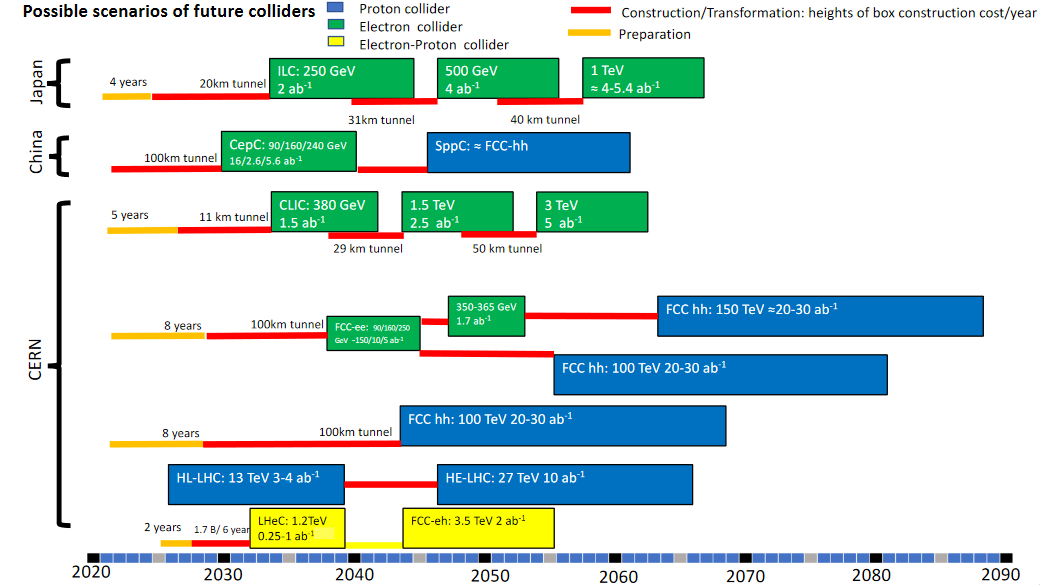
\includegraphics[width = 0.95\textwidth]{IMG/Cap1/Roadmap.png}
	\caption{Possible  timelines  of  future  colliders.  It includes high-energy $e^+e^-$ (ILC,  CLIC,  CEPC  and  FCC-ee), $pp$ (FCC-hh  and HL-LHC) and $e-p$ (LHeC and FCC-eh) machines. Image from \cite{roadmap}.}
	\label{fig:roadmap}
\end{sidewaysfigure}

\subsection*{Future Circular Collider $e^+e^-$}
A post-LHC circular collider at CERN has been proposed with the name of Future Circular Collider (FCC) project \cite{FCC}. FCC is staged in a first lepton collider (FCC-ee) \cite{FCC-ee} phase followed by a hadron collider (FCC-hh) \cite{FCC-hh} with a final target centre-of-mass energy of $100$ TeV. A common tunnel, about $100$ km long, is designed to host both of them. With this choice the same facility could potentially house an electron-hadron collider.\\
FCC-ee is designed to provide the highest possible statistics for the $Z$, $W$ and $H$ bosons, and $t$ quarks. At present, it is supposed to operate at centre-of-mass energies ranging from $88$ to $365$ GeV in four different ($\sqrt{s}$) operating points:
\begin{itemize}
    \item $\simeq 91$ GeV, corresponding to the $Z$ pole;
    \item $\simeq 160$ GeV, corresponding to the $W^+W^-$ production threshold;
    \item $\simeq 240$ GeV, corresponding to the $ZH$ production threshold;
    \item $\simeq 340-365$ GeV, corresponding to the $t\Bar{t}$ threshold.
\end{itemize}

The FCC-ee project fits over the present CERN accelerator complex, where the injector chain makes use of a $6$ GeV linac, a damping ring and the CERN SPS as a pre-booster. The baseline layout, sketched in Figure \ref{fig:FCC-ee}, is designed with two different interaction points.\\
The task of increasing our knowledge of many of the electroweak observables by one or two orders of magnitude better than the current one sets challenging constrains to the integrated luminosities needed. These values range from $0.2$ ab$^{-1}$, for the measurement of the top-quark mass and width, to $100$ ab$^{-1}$, for the measurement of the effective weak mixing angle.
These luminosities can be achieve in a reasonable amount of time only by circular colliders (see Figure \ref{fig:FCC-ee_lum}). 

\begin{figure}
	\centering
	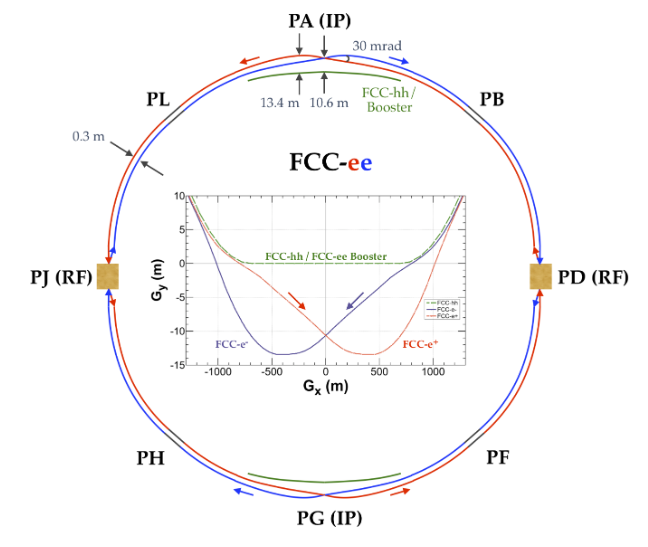
\includegraphics[width=.65\textwidth]{IMG/Cap1/FCC-ee.png}
	\caption{Schematic view of the FCC-ee. Image from \cite{FCC}.}
	\label{fig:FCC-ee}
\end{figure}

\begin{figure}
	\centering
	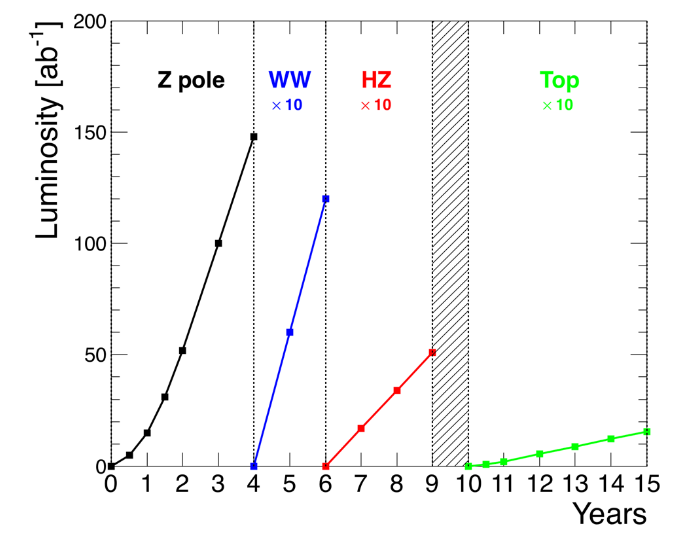
\includegraphics[width=.7\textwidth]{IMG/Cap1/FCC-ee_lum.png}
	\caption{Integrated FCC-ee luminosity during 15 years of operation. Image from \cite{FCC-ee}.}
	\label{fig:FCC-ee_lum}
\end{figure}

\subsection*{Circular Electron Positron Collider}
The Circular Electron Positron Collider (CEPC) is an international project initiated and hosted by China addressing high-luminosity $e^+e^-$ collisions. It is designed to operate at centre-of-mass energies of $240$ GeV (as an $H$ factory exploiting the $e^+e^- \rightarrow ZH$ process), $91.2$ GeV ($Z$ pole) and $160$ GeV ($W^+W^-$ threshold).\\

The present design, similarly to the FCC-ee, foresees a double ring structure, sketched in Figure \ref{fig:CEPC} with a circumference of $100$ km and two interaction points. The same $100$ km-long tunnel could also host a Super Proton-Proton Collider (SPPC) which, without removing the CEPC ring, gives the possibility to perform electron-proton collisions. As described in the conceptual design report \cite{CEPC_design1, CEPC_design2}, the main accelerator is preceded by a linear accelerator, a damping ring and a booster.\\
Associated to the three operating $\sqrt{s}$ values the instantaneous luminosities are expected to reach $3 \times 10^{34}$, $32 \times 10^{34}$ and $10 \times 10^{34}$ cm$^{-2}$s$^{-1}$, respectively.
CEPC will produce, over is planned operative time, large samples (more than one million) of Higgs, one trillion of $Z$ bosons and about 100 million of $W^+W^-$ events, allowing precise measurements of many electroweak parameters.\\

\begin{figure}
	\centering
	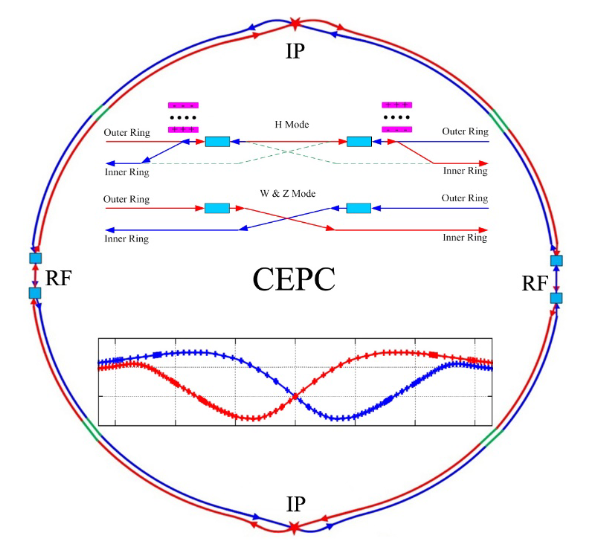
\includegraphics[width=.65\textwidth]{IMG/Cap1/CEPC.png}
	\caption{Schematic view of the CEPC. Image from \cite{CEPC_design2}.}
	\label{fig:CEPC}
\end{figure}

According to \cite{CEPC_schedule}, the CEPC construction could possibly start within few years in order to be completed by 2030, a very aggressive time schedule compared to the other collider proposals.

\subsection*{International Linear Collider}
The ILC is an $e^+e^-$ linear collider that, at the current state (ILC250), provides a $250$ GeV centre-of-mass energy.
The ILC accelerator is based on SuperConducting RadioFrequency (SCRF) cavities already in use at the European X-ray Free Electron Laser facility (E-XFEL), located at DESY/Hamburg.\\

The design luminosity is $1.35-1.5 \times 10^{34}$ cm$^{-2}$s$^{-1}$ at $E_{cm} = 250$ GeV with a corresponding integrated luminosity ranging from $400$ fb$^{-1}$ (in the first years) up to $2$ ab$^{-1}$ (after future upgrades).
The ILC250 is $20.5$ km long with two main arms, mostly occupied by the electron and positron linacs, at a $14$ mrad crossing angle. The ILC candidate site is in the Kitakami region in northern Japan. A sketch of the ILC250 is shown in Figure \ref{fig:ILC250}.\\
In its current state, the SCRF cavities will reach frequency values of $1.3$ GHz providing a gradient of $31.5-35$ MV$/$m while operating in a cryogenic infrastructure at $2$ K.\\

The first stage of ILC has the task to measure the $H$ parameters and its model-independent determination by studying the $e^+e^- \rightarrow ZH$ collisions at $\sqrt{s}= 250$ GeV.
Two energy upgrades are currently foreseen for extending the centre-of-mass energy to $500$ GeV and $1$ TeV.
The main goals for the higher-energy physics runs cover improved precision measurements of the top-quark mass, the top-quark electroweak couplings, the Higgs coupling to the top quark, and the triple-Higgs coupling \cite{ILC_global_project}.\\

\begin{figure}
	\centering
	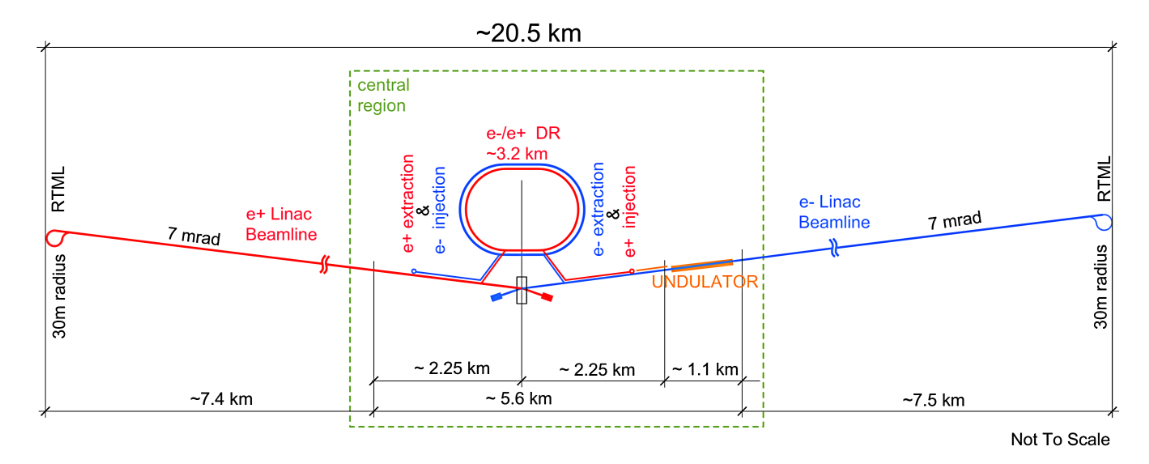
\includegraphics[width=.8\textwidth]{IMG/Cap1/ILC.png}
	\caption{Schematic layout of the ILC at $250$ GeV staged option \cite{ILC_global_project}.}
	\label{fig:ILC250}
\end{figure}

\subsection*{Compact Linear Collider}
The Compact Linear Collider (CLIC) is a TeV-scale high-luminosity linear leptonic collider to be located in the CERN area. The CLIC energy stages, at present, comprises 3 working points, at $\sqrt{s}= 380$ GeV, $1.5$ TeV and $3.0$ TeV, with corresponding instantaneous luminosities of $1.5$, $3.7$ and $5.9 \times 10^{34}$ cm$^{-2}$s$^{-1}$, respectively. The site length will have to scale, in these stages, from $11$ km up to $50$ km.\\

The CLIC project, proposed in 2012 \cite{CLIC_old1, CLIC_old2, CLIC_old3} and updated in 2016 \cite{CLIC_update}, will adopt a two-beam acceleration scheme as shown in Figure \ref{fig:CLIC}, where the electron and positron beams are independently accelerated through the whole chain.\\
In the first stages, particles are accelerated to $9$ GeV using a linac booster. Then they are injected in normal-conducting high-gradient $12$ GHz accelerating structures. The two main linacs accelerate beams exploiting normal-conducting $X$-band cavities with an accelerating gradient of $100$ MV$/$m, the highest among linear colliders. To reach these extremely high accelerating gradients, a novel drive-beam scheme, using low-frequency klystrons to generate long RF pulses and store their energy in a long, high-current, drive-beam pulse, is designed. This beam pulse is used to generate several short pulses distributed along the main linac.

\begin{figure}
	\centering
	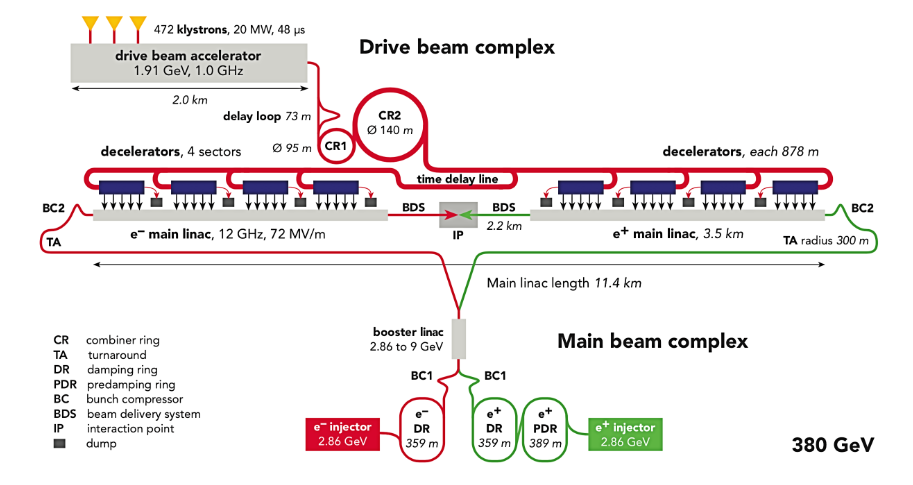
\includegraphics[width=.8\textwidth]{IMG/Cap1/CLIC.png}
	\caption{Schematic layout of the CLIC at the 380 GeV staged option \cite{CLIC_img}.}
	\label{fig:CLIC}
\end{figure}

\section{IDEA Detector concept} \label{sec:Idea_project}
IDEA (Innovative Detector for Electron-positron Accelerators) is an innovative multi-purpose detector concept, designed to study electron-positron collisions in a wide energy range as provided by high-luminosity electroweak factories.
The detector concept was proposed in 2017 and included in conceptual design reports of both FCC-ee \cite{FCC-ee_design} and CEPC \cite{CEPC_design}.

\begin{figure}
	\centering
	\subfloat[][ Artistic view of the IDEA detector concept. \label{fig:IDEA_art1}]{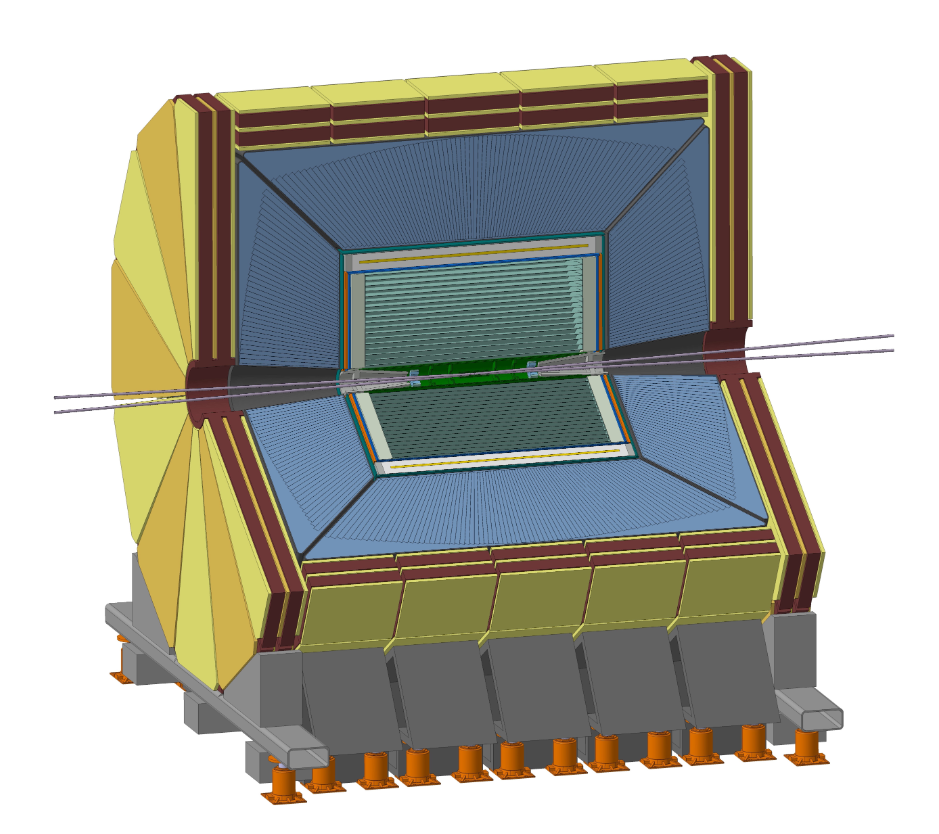
\includegraphics[width=.45\textwidth]{IMG/Cap1/IDEA_art1}} \quad
	\subfloat[][The structure and dimensions of the IDEA detector concept. \label{fig:IDEA_art2}]{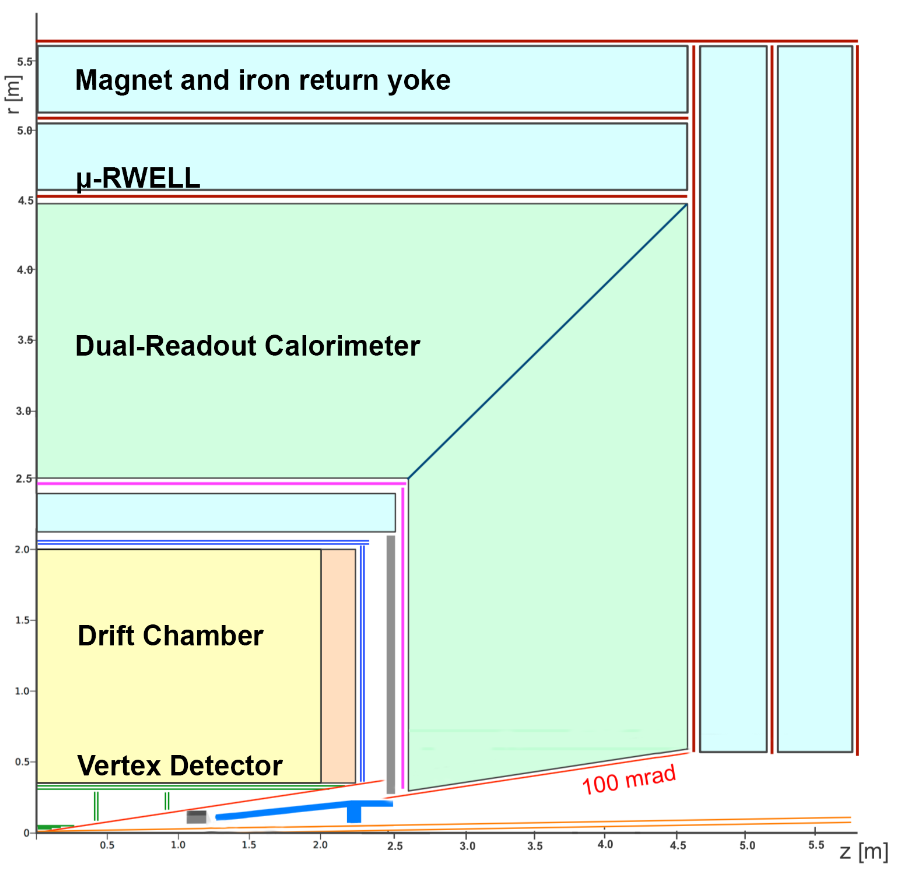
\includegraphics[width=.45\textwidth]{IMG/Cap1/IDEA_art2}}
	\caption{The IDEA detector concept.}
\end{figure}

The IDEA Detector concept is sketched in an artistic view in Figure \ref{fig:IDEA_art1} and in its structure and dimensions in Figure \ref{fig:IDEA_art2}. 
The overall detector is composed by a silicon pixel vertex detector, a wire chamber surrounded by a layer of silicon micro-strip detectors, a thin superconducting solenoid coil, a preshower detector, a dual-readout calorimeter and a muon spectrometer.
The most innovative elements proposed are:
\begin{itemize}
  \item an ultra-light drift chamber as main tracker;
  \item a Dual-Readout (DR) fibre-sampling calorimeter, for both electromagnetic and hadronic shower measurement.
\end{itemize}

The Drift CHamber (DCH) technology is based on the R\&D work done for the upgrade of the MEG experiment (MEG II), designed to search for the charged lepton flavor violating decay $\mu \rightarrow e\gamma$. This work involves the construction of an ultra-light drift chamber performing high momentum resolution and high transparency in terms of radiation length.
The IDEA dual-readout calorimeter, on the other hand, stands on the legacy of the DREAM/RD52 Collaboration. The key point is the expected performance of dual-readout optical-fibre calorimeters in obtaining high-resolution energy measurements for both single hadrons and hadronic jets.
All the most important parameters of the IDEA detector components are listed in Table \ref{tab:IDEA_part}.\\
\begin{table}
  \centering
  \begin{tabular}{ll}
    \toprule
    Vertex technology                       & Silicon \\
    Vertex inner/outer radius (cm)          & $1.7/34$ \\
    \midrule
    Tracker technology                      & Drift Chamber and Silicon Wrapper\\
    Tracker half length (m)                 & $2.0$ \\
    Tracker outer radius (m)                & $2.0$ \\
    \midrule
    Solenoid field (T)                      & $2.0$ \\
    Solenoid bore radius / half length (m)  & $2.1/30.$ \\
    \midrule
    Preshower absorber                      & Lead \\
    Preshower $R_{min}/R_{max}$ (m)         & $2.4/2.5$ \\
    \midrule
    Calorimeter absorber                    & Copper \\
    Calorimeter $R_{min}/R_{max}$ (m)       & $2.5/4.5$ \\
    \midrule
    Overall height / length (m)             & 11/13 \\
    \bottomrule
  \end{tabular}
  \caption{Parameters of the different sub-detectors composing IDEA.}
  \label{tab:IDEA_part}
\end{table}

\subsection{Vertex detector}
The $1.5$ cm beam pipe is surrounded by the IDEA vertex detector composed by pixel active sensors. The structure present a high-resistivity substrate architecture implementing on-pixel sparsification and data-driven, time-stamped readout.
The goal is a thickness of $0.15-0.30\%\ X_0$ per layer and a power dissipation below $20$ mW$/$cm$^2$.

The tracks of charged particles are measured with very high precision, of the order of $3$ $\mu$m in the innermost layers. The vertex detector must also be able to precisely reconstruct secondary vertices.
%This detector will significantly benefit from the electronic and mechanical work for the ALICE ITS \cite{alice_its}, as well as of new ongoing developments, in the framework of the INFN ARCADIA R\&D project.
%%%

\subsection{Drift chamber}
Based on the experience with the KLOE Experiment DCH \cite{KLOE} and the recent DCH for the MEG upgrade \cite{MEG2}, a similar detector, with extraordinary transparency to charged particles, has been proposed for the IDEA Experiment.\\

The chamber is composed by a unique cylindrical volume, coaxial to the beam axis, with an inner radius of $0.35$ m and an outer radius of $2$ m, for a total length of $4$ m. It consists of $112$ coaxial layers, at alternating-sign stereo angles, grouped in $24$ identical sectors. The total number of drift cells is $56448$ with variable size from $12.0$ to $14.5$ mm.
The chamber is operated with a very light gas mixture of $90\%$ He - $10\%$ iC$_4$H$_{10}$ (isobutane), providing a maximum drift time value of $\simeq 400$ ns.\\
The angular coverage extends down to $\simeq 13\deg$, and could be extended with additional silicon disks between the DCH and the calorimeter end caps.\\
In the radial direction the total amount of material is of the order of $1.6\%$ of a radiation length ($X_0$), including the inner and outer cylindrical walls and the contributions due to the gas mixture and the wires. On the other hand, in the forward and backward direction, the total amount of material is equivalent to about $5.0\%\ X_0$, including the inner cylindrical walls and the service end plates, instrumented with front-end electronics, signal and HV cables.\\

In the context of the MEG2 drift chamber prototypes \cite{MEG2} with $7$ mm cell size, a drift distance resolution of $100$ $\mu$m has been achieved with both a gas mixture and operating conditions very similar to the ones foreseen for the IDEA DCH.
Analytical calculations, in such operating conditions, were used to estimate the momentum and angular resolutions with the results shown in Figure \ref{fig:DCH_res}.
The drift chamber also offers outstanding particle-identification performance using the cluster counting technology that improves, as well, the spatial resolution.

%Together with the excellent expected momentum resolution, the DCH can achieve superior particle identification capabilities thanks to the cluster-counting technique.
The ionisation process, by means of which electrons are released, follows a Poison law, therefore, by counting the total number of ionisation clusters ($N_{cl}$) of a charged track, one can reach a relative resolution on $N_{cl}$ that scales as  $1/\sqrt{N_{cl}}$. The expected performance relative to particle separation, in terms of number of standard deviations as a function of the particle momentum, is shown in Figure \ref{fig:DCH_separation}. In this graph the solid curves refer to the cluster-counting technique, while the dashed ones refer to the expected identification power for the traditional $dE/dx$ method. As it can be seen, the particle separation by cluster counting performs better over the whole momentum range.

\begin{figure}
	\centering
	\subfloat[][Momentum and angular resolutions for $\theta= 90^{\circ}$ as a function of particle momentum. \label{fig:DCH_res}]{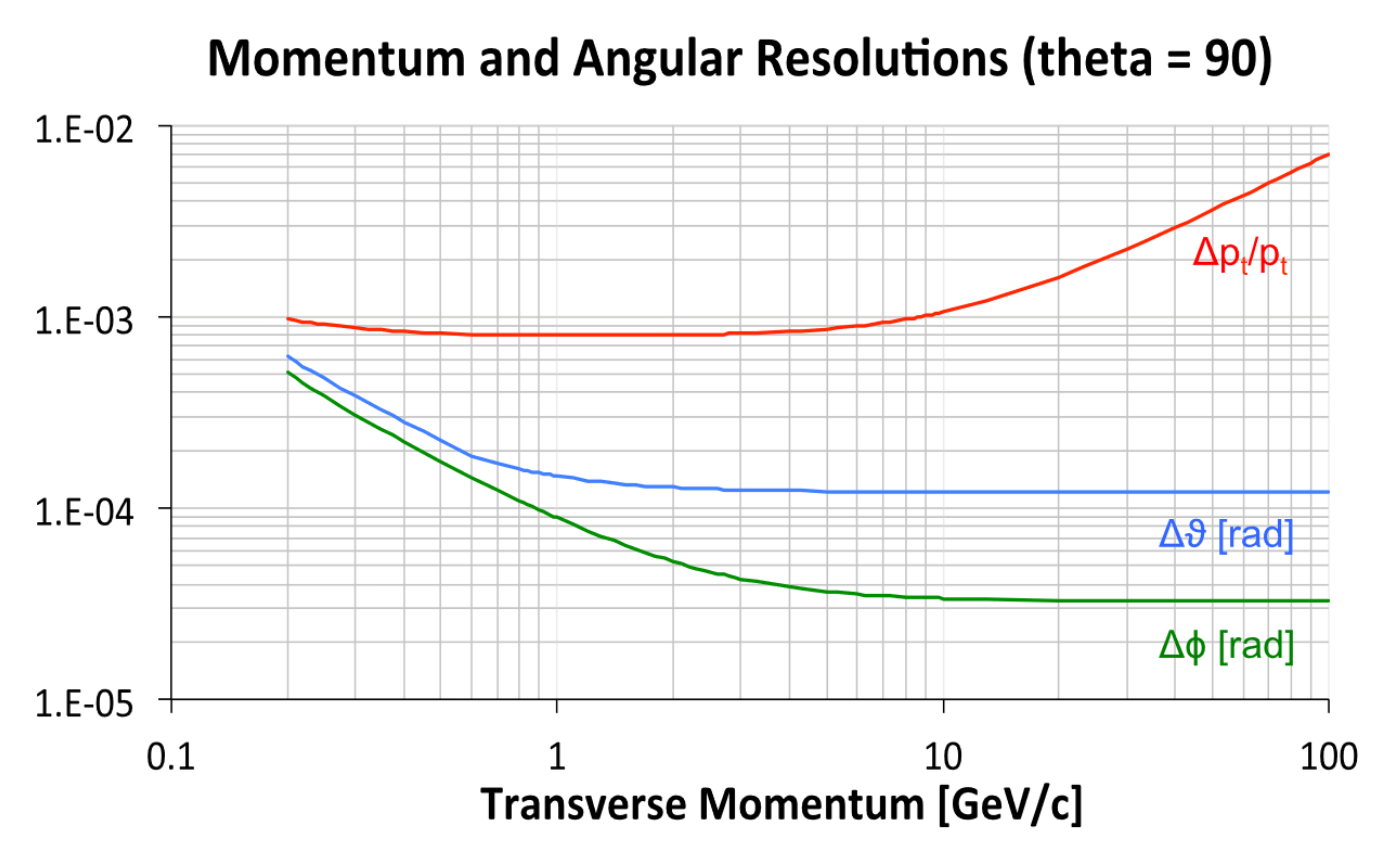
\includegraphics[width=.45\textwidth]{IMG/Cap1/DCH_res.png}} \quad
	\subfloat[][Particle-type separation in units of standard deviations as a function of momentum, with cluster counting (solid curves) and with $dE/dx$ (dashed curves). \label{fig:DCH_separation}]{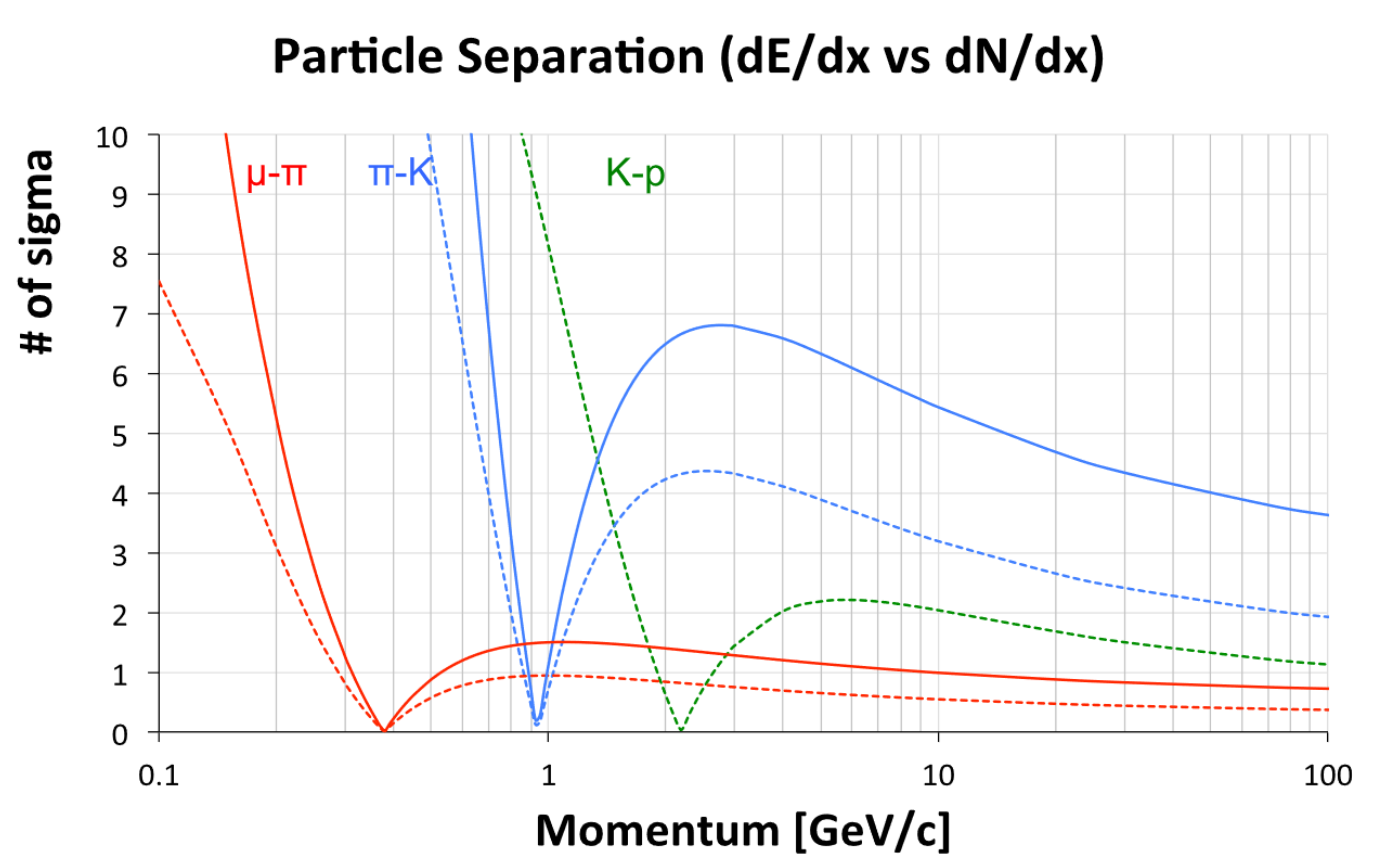
\includegraphics[width=.45\textwidth]{IMG/Cap1/DCH_separation.png}}
	\caption{IDEA ultra-light drift-chamber performance \cite{FCC-ee_design}.}
\end{figure}

\subsection{Magnet system}
The IDEA detector magnet is an ultra-thin and ultra-light (thus “radiation-transparent”) superconducting solenoid. It is $5$ m long and has an inner diameter of $4.2$ m. The main feature is that the solenoid is positioned between the tracking detectors and the calorimeter, a solution currently employed in ATLAS.
This choice requires to mantain the total thickness at the $30$ cm level, and below $1\ X_0$ in terms of radiation length, but at the same time the stored energy is reduced by a factor of four and the cost can be halved.
In this scenario a relatively low field of $2$ T can be produced.
%The flux return yoke scales with the square of the coil diameter, thus with the given dimensions a yoke thickness of less than $100$ cm of iron is sufficient to contain the magnetic flux and to shield the muon chambers.

\subsection{Dual-readout calorimeter}
The IDEA calorimeter consists of a dual-readout projective fibre-sampling detector. It follows the lessons of the high-resolution fibre calorimeters built by SPACAL \cite{SPACAL} and RD52 \cite{RD52}.\\
The detector is a tower-based, longitudinally unsegmented, fully projective calorimeter sketched in Figure \ref{fig:DRCal_geo}.
%The detector is a $4\pi$ calorimeter that does not present segmentation longitudinally, but only in the direction towards the Interaction Point (IP).
The segmentation is chosen to have the shower development confined in a small number of towers and most of the energy deposited in a single tower.
This highly simplifies the calibration procedures for which each cell response can be considered individually.
Considering that in accelerator-based experiments all the particles come, in good approximation, from the Interaction Point (IP), the projective segmentation can be obtained with a tower-based structure.\\

DR calorimeters, as described in Section \ref{sec:DRComp}, are composed by an absorber and two different active media to induce and transport two different signals. A single medium with two different response processes (such as a crystal producing both scintillation and Cherenkov light) may also be used.
In the IDEA DR calorimeter, a copper (or brass) matrix is used as absorber, filled with optical fibres as active volumes (the dual-readout method will be described in the next chapter).
The possibility to independently read out each fibre with a dedicated Silicon PhotoMultiplier (SiPM), as described in \cite{Massi_tesi}, brings a series of advantages especially in terms of spatial and angular resolution, removing the limitations arising from a readout driven by the tower dimension. For example, two particle showering in the same tower, in this way, could still be identified.\\

\begin{figure}
	\centering
	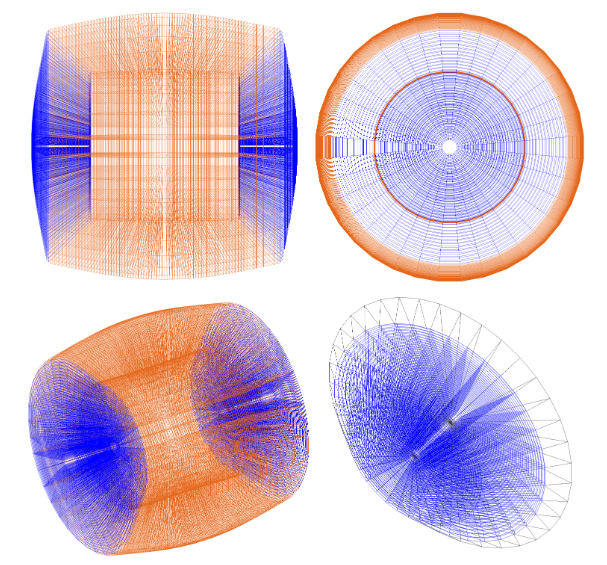
\includegraphics[width=.9\textwidth]{IMG/Cap1/DRCal_geo.png}
	\caption{IDEA dual-readout calorimetry geometry produced with GEANT4, seen from different perspectives. In orange the towers composing the barrel, in blue the ones composing the end caps.}
	\label{fig:DRCal_geo}
\end{figure}

The geometry of the calorimeter, from different perspectives, is shown in Figure \ref{fig:DRCal_geo}. Towers are truncated pyramids pointing to the IP. In such a way, each tower cover a specific region $(\Delta \theta, ~\Delta\varphi)$ of the solid angle.\\
The cylindrical symmetry is achieved through a rotation around the beam axis of a minimal structure called slice. A single slice covers a range of $10\degree$ of the $\varphi$ angle, therefore $36$ of these elements cover the full calorimeter volume.
In each slice both barrel and end-cap towers are present, in particular $80$ towers for the barrel and $35$ for each end cap, with an approximate $\theta$ coverage of $1.125\degree$ per tower.\\
All the towers are $2$ m long, composed by an absorber matrix (copper, in the actual simulation) filled with optical fibres.
The active elements are scintillating (polystyrene) and clear-plastic fibres (PolyMethyl MethAcrylate - PMMA).
The fibres are $\sim 1$ mm thick and are disposed in a chess-board like geometry so that each fibre is separated from the closest ones by $\sim 0.5$ mm of absorber material.
This complex geometry has been reproduced within the GEANT4 simulation toolkit \cite{GEANT4} and all results in this thesis are obtained with it.

\subsection{Preshower and muon chambers}
In the barrel region, just before the calorimeter, the magnet coil, coupled with Micro-Pattern Gaseous Detector (MPGD) chambers, acts as a preshower.
In the forward regions, preshower detectors are located between the drift chamber and the end-cap calorimeters.
Externally, the overall detector is surrounded by an iron return joke, to contain the magnetic field, and this volume is also instrumented with MPGD chambers, to allow muon detection and momentum measurement.
Both the preshower and the muon chambers are based on the micro-Resistive WELL ($\mu$-RWELL) technology. $\mu$-RWELL chambers are compact MPGD detectors, with a single, intrinsically spark protected, amplification stage. \\
The evaluation of the preshower performance and the single-hit-position resolution requirement are still in progress.
However, experimental results with small prototypes already show a good acceptance for photons and an efficiency of $\simeq 30\%$ for tagging $\pi^0$ from their $\gamma\gamma$ decay.\\
Also the requirements for the muon system look to be within reach. Indeed, this technology provides good tracking efficiency, high-voltage stability, a position resolution of $200-300$ $\mu$m and a good time resolution, thanks to the fast charge amplification process.\\
%Also the muon detector uses as well the $\mu$-RWELL technology but with a wider strip pitch, due to the greater dimensions. It is subdivided in three active layers at increasing distance from the vertex, and located within the iron return yoke that closes the magnetic field. Each MPGD can provide a space point with a spatial resolution of about $400$ $\mu$m in the plane perpendicular to the particle direction. Combining the three stations allows to perform standalone tracking of charged particles at $5-6$ m from the vertex. Such a precision also allows to identify secondary vertices that could be produced by long lived particles.

		
		%---------CAPITOLO 2--------
		%\chapter{Calorimetry and dual-readout}
Calorimetry is an important detection principle in particle physics.
Originally developed with astrophysical purpose for cosmic-ray studies, this method refers to the detection of particles and the measurement of their properties, using blocks of instrumented material.
It was developed and perfected for accelerator-based particle physics experimentation primarily in order to measure the energy of particles. 
In these blocks, particles are fully absorbed and their energy transformed into a measurable quantity.\\
The incident particle interact with the detector (through electromagnetic or strong processes) producing a shower of secondary particles with progressively degraded energy.
The energy deposited by the charged particles of the shower in the active material of the calorimeter, which can be detected in the form of charge or light, is used to measure the energy of the incident particle.
Typical processes suitable to detect this energy are: ionization of the medium, scintillation light and the Cherenkov light produced by relativistic particles.\\

Calorimeters can be divided into two categories depending on the type of shower they are optimized to detect: electromagnetic calorimeters, used mainly to measure electrons and photons through their electromagnetic interactions (e.g.
bremsstrahlung, pair production), and hadronic calorimeters, used to measure mainly hadrons through their strong and electromagnetic interactions.\\
Another classification can be made according to their construction technique defining sampling calorimeters and homogeneous calorimeters.\\
Homogeneous calorimeters are built of one type of material that performs both the main tasks: degrade the energy of the incident particles and provide the detectable signal.\\
Sampling calorimeters, instead, consist of alternating layers of an absorber, a dense material used to perform energy degradation, and an active medium that generate the signal.\\

%Calorimeters are attractive in high-energy particle physic field for various reasons:
%\begin{itemize}
%		\item In most cases the calorimeter energy resolution improves with energy as $1/\sqrt{E}$, where $E$ is the energy of the incident particle. Therefore calorimeters are very well suited to high-energy physics experiments.
%		\item Calorimeters are sensitive to all types of particles, charged and neutral (e.g., neutrons). Also neutrinos and their energy can be indirectly detected can even provide indirect detection of neutrinos and their energy through the measurement of the event missing energy.
%		\item They are versatile detectors. They can be used to determine the shower position and direction, to perform particle identification, to measure the arrival time of the particle, or even to provide fast signals useful in trigger purpose.
%		\item They are space and therefore cost effective. Because the shower length increases only logarithmically with energy, the detector thickness needs to increase only logarithmically with the energy of the particles.
%\end{itemize}

This chapter describes the physics behind both the electromagnetic and hadronic shower developments, provides a basic description of the energy response of these detectors and introduces the particular technique of the dual-readout, a modern concept of calorimeter that has the quality of overcome the non-compensating problem measuring both electromagnetic and hadronic showers through two different type of signals simultaneously (Cherenkov and scintillation light).\\

A more comprehensive descriptions of the topic can be found in the references \cite{Wigmans_book} and \cite{Gianotti_article}.

\section{Physics of shower development}
A particle interact and lose part or whole of its energy traversing matter. During this process the medium get excited and heated up, is excited in this process, or heated up. From this feature the term calorimetry, literally meaning "heat measurement", was introduced.\\
The groundwork for the calorimetry is the interaction processes between particle and matter. They are the manifestation of the electromagnetic, the strong and, more rarely, the weak forces and they strongly depend on the energy and the nature of the incident particle, in addition to medium features.\\
The term particle shower refers to the production of a group of particles generated by the interaction of a primary particle with the matter. The processes and the consequent shower effects are the keys to deeply understand this topic.\\

\subsection{Electromagnetic showers} \label{subsec:em_shower}
Despite the complex mechanisms of particle-matter interaction, electromagnetic showers are produced via a small number of well understood QED processes. Charged particles (electrons and positrons) lose energy by ionization and by radiation, instead neutral ones (photons) are characterized by photoelectric effect, Compton scattering and pair production.\\

The first type of particle in its path through the medium ionize it under the condition of having an energy at least sufficient to release the atomic electrons from the Coulomb fields generated by the atomic nuclei (few of $eV$).
The amount of energy released (in unit of path) by these particle is predictable through the semi-empirical Bethe-Block formula restricted to electrons (and positrons) \cite{Leo}:
\begin{equation}
    -\frac{dE}{dx} = 2\pi N_a r_e^2 m_e c^2 \rho \frac{Z}{A}\frac{1}{\beta^2}\left[ \ln{\frac{\tau^2(\tau + 2)}{2(I/m_ec^2)^2}} -F(\tau) -\delta -2\frac{C}{Z}\right]
\end{equation}
the stopping power (i.e. the quantity described by the formula) decreases as the particle energy increases ($\propto \beta^2$). Hence the ionization process is the greatest source of energy loss for particles with small energy.\\
The other energy loss process known as \textit{bremsstrahlung} is the dominant source of energy loss by electrons and positrons at energies above $100\ MeV$. Relativistic electrons and positrons radiate photons as a result of the interaction between Coulomb and the atomic electric fields. The energy spectrum of these photons falls off as $1/E$ ranging till the primary particle energy, but in general most of the photons carry a small part of it.
The process produces (usually small) changes in electron (or positron) direction. This is called Coulomb or multiple scattering.\\
At a fixed energy the relative importance of ionization and radiation losses depends on the medium and in particular on the electron density of the medium in which the shower develops. This density is in first approximation proportional to the (average) $Z$ of the medium.
The critical energy, i.e. the energy value at which the two processes have equal impact, is roughly inversely proportional to the $Z$ value of the material:
\begin{equation}
    \varepsilon_c = \frac{160\ MeV}{Z + 1.24}.
\end{equation}
An example of energy loss in copper by electron is sketched in figure \ref{fig:Cu_rad_ion}, where the ionization and radiation contribution are separated.\\

\begin{figure}
	\centering
	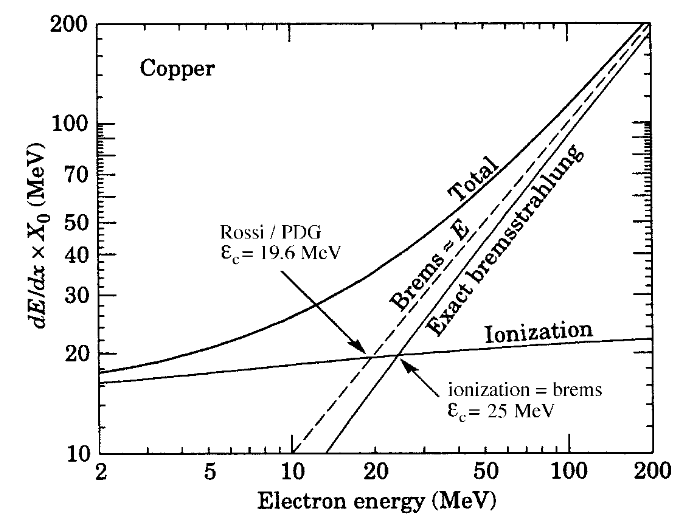
\includegraphics[width=0.8\textwidth]{IMG/Cap2/Cu_rad_ion}
	\caption{Energy losses through ionization and bremsstrahlung by  electrons in copper. From [PDG 98].}
	\label{fig:Cu_rad_ion}
\end{figure}

The other particles that produce electromagnetic showers are photons. The interaction between photons and matter is mainly affected by three different processes: the photoelectric effect, Compton scattering and electron–positron pair production.\\

The photoelectric effect is the process that most likely occurs at low energies. It is characterized by an atom absorbing the photon and emitting an electron. Eventually the atom, left in an excited state, emits an Auger electrons or X-rays returning to the ground state. The photoelectric cross section strongly depends on the available number of  electrons,  and  thus  on  the $Z$ value  of  the  absorber  material. In particular it scales with $Z^n$, with the power $n$ between 4 and 5. Meanwhile the photoelectric cross section rapidly decrease with greater energies, varying as $E^{-3}$. In this way the process rapidly loses its impact as the energy increases. %Quantitatively, in uranium ($Z=92$) the cross section for photoelectric effect is dominant for energies below $700\ keV$, meanwhile for iron  ($Z=26$) decreases his importance from $100\ keV$.\\

The Compton process is a scattering process where an impinging  photon interact with an atomic electron transferring enough momentum and energy to the struck electron to escape from the atomic Coulomb field. Kinematic variables such as energy transfer and scattering angles can be easily obtained applying the laws of energy and momentum conservation. 
% The dynamic is illustrated in Figure \ref{fig:scatt_kin}. 

%\begin{figure}
%	\centering
%	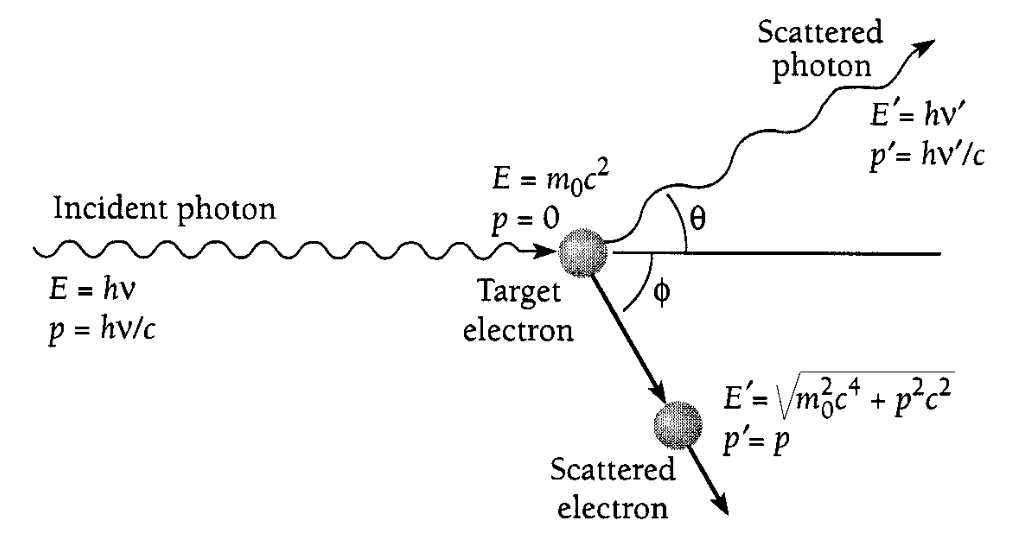
\includegraphics[width=0.8\textwidth]{IMG/Cap2/scatt_kin.png}
%	\caption{Compton scattering process. Image from \cite{Leo}.}
%	\label{fig:scatt_kin}
%\end{figure}

%The photon is absorbed and thus disappears in the photoelectric effect, but it only plays a role at low $\gamma$ energies.
Photons in the $MeV$ energy range are absorbed by photoelectric effect only after a sequence of Compton scattering processes, in which the photon energy is reduced step by step in each collision until it is low enough to permit the photoelectric occurrence. In each step, the amount of loss energy is:
\begin{equation}
    T = E_{\gamma}\frac{\xi(1 - \cos{\theta})}{1 + \xi(1 - \cos{\theta})}
\end{equation}
where $\xi = E_{\gamma}/m_ec^2$.
The cross section linked to the Compton scattering is much less dependent on the $Z$ value than the photoelectric one. It is almost proportional to the number of target electrons in the nuclei. Also in this process the cross section decreases with increasing photon energy, but only with the first power of $E$. Therefore Compton scattering has more impact than photoelectric absorption above a certain threshold energy. %This  threshold varies from $20\ keV$ for carbon ($Z=6$) to $700\ keV$ for uranium ($Z=92$).\\

The pair production process, differently from the previous ones, has a binding threshold under which the effect can not occur. This threshold is the twice of the electron rest mass ($2\times 511\ MeV$). If the photon has a higher energy then it can produce an electron-positron pair that can continue the path in the medium producing bremsstrahlung radiation as well as ionization.
%The electron can be eventually absorbed by an ion, while the positron annihilates with an electron producing two new photons, each with an energy of $511\ keV$.

The cross section for pair production rises with the energy reaching an asymptotic value at higher then $1\ GeV$. For this reason, at high energies, pair production is the most likely process to occur. Meanwhile the dependence from the medium goes, in first approximation, as $Z^2$.\\

Comparing the cross section of the three processes and its dependence with respect to the photon energy it is clear that the photoelectric effect dominates at lower energies, meanwhile at the intermediate values the Compton scattering gives the greatest contribute, at the end at higher energies almost every photon loses its energy through pair production. An example of these contributions is shown in figure \ref{fig:ph_cross_E}.\\
Knowing the dependence of the cross sections with respect to the $Z$ of the material, ranges of energies where each process dominates can be found and parametrized with the $Z$ value. A representation is sketched in figure \ref{fig:ph_cross_Z}.

%\begin{figure}
%	\centering
%	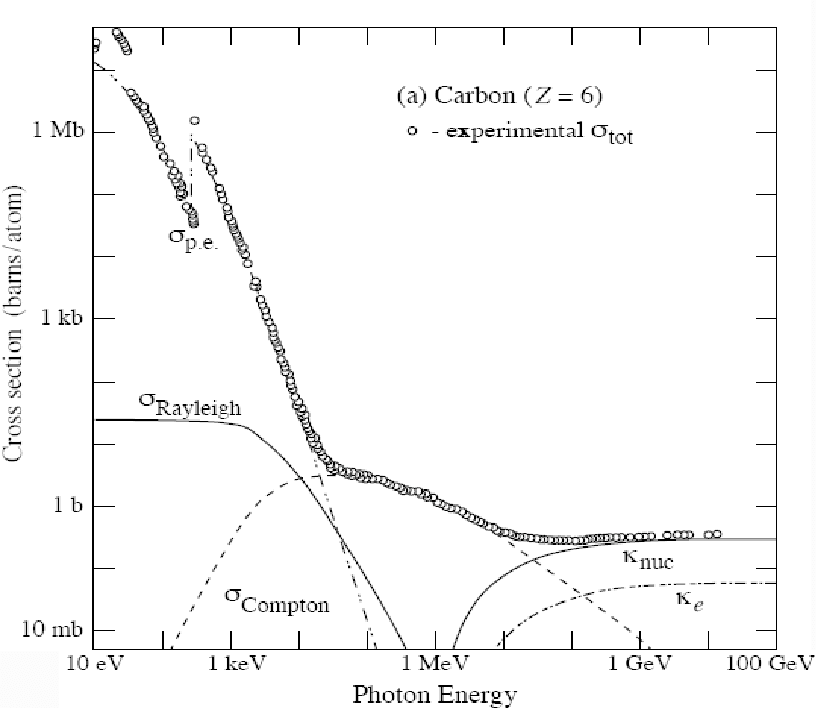
\includegraphics[width=0.7\textwidth]{IMG/Cap2/ph_cross_E.png}
%	\caption{Compton scattering process. Image from \cite{Leo}.}
%	\label{fig:ph_cross_E}
%\end{figure}
%\begin{figure}
%	\centering
%	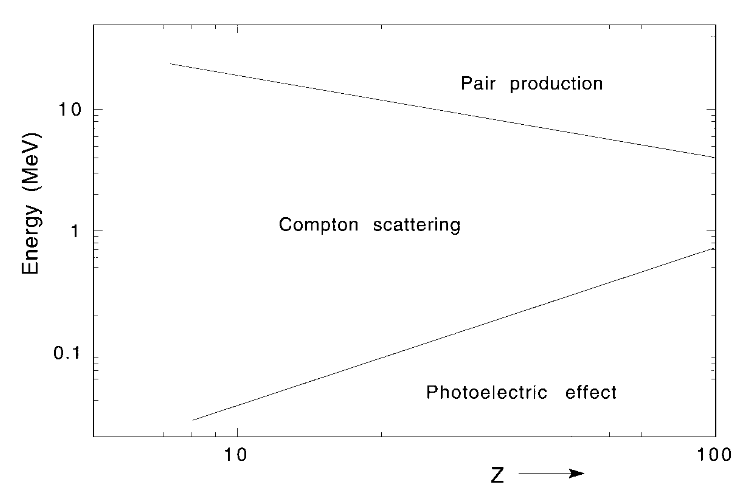
\includegraphics[width=0.7\textwidth]{IMG/Cap2/ph_cross_Z.png}
%	\caption{Compton scattering process. Image from \cite{Leo}.}
%	\label{fig:ph_cross_Z}
%\end{figure}

\begin{figure}
	\centering
	\subfloat[][Total cross section of photon in Carbon. Different processes contribution are also separated. \label{fig:ph_cross_E}]{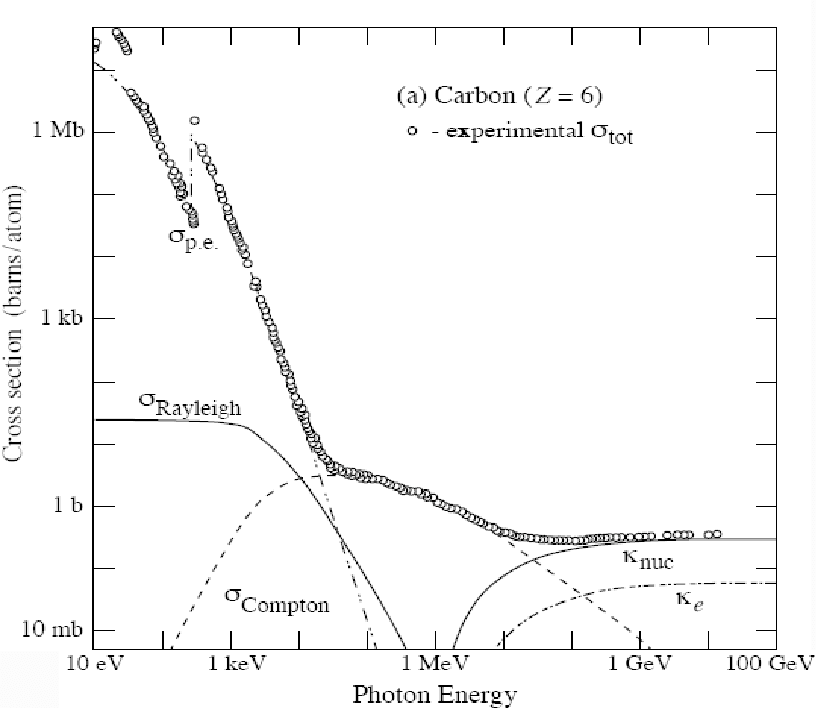
\includegraphics[height=.18\textheight]{IMG/Cap2/ph_cross_E.png}} \quad
	\subfloat[][Energy ranges where different processes dominate with respect to the medium $Z$ value.\label{fig:ph_cross_Z}]{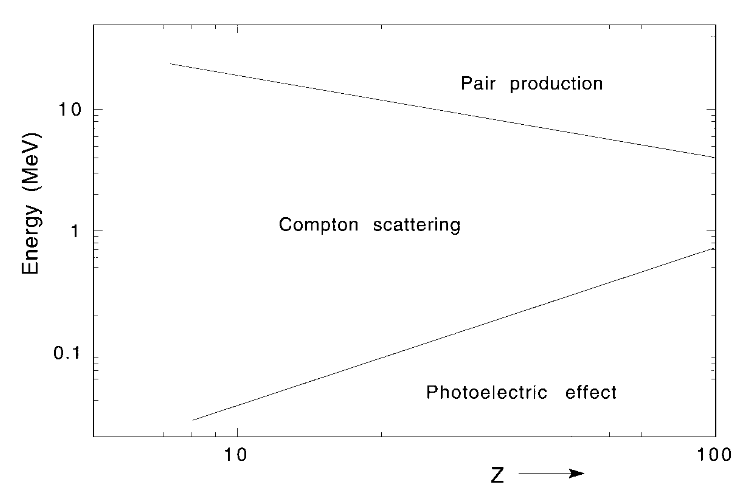
\includegraphics[height=.18\textheight]{IMG/Cap2/ph_cross_Z.png}}
	\caption{Images from \cite{Leo}.}
	%\label{fig:sigma_su_e}
\end{figure}

\subsubsection*{Shower principle}
Minimal showers may also develop at vary low energy of primary particle. Starting for example from a photon of tens of $MeV$, it can eventually produce a electron-positron pair in the calorimeter. The  charged  particles lose their energy in the matter through ionization. When the  positron loses all the kinetic energy, it annihilates with an electron producing two $511\ keV\ \gamma$s. These photons are absorbed through the photoelectric effect after a sequence of Compton scattering. During the process, the energy of the primary particle is released to the material by charged particle in ionization processes.\\
At energy values of $1\ GeV$ and higher, electrons, protons and photons initiate actual electromagnetic showers in the materials in which they penetrate. At these energies charged particles lose their energy mostly by brehemstralung, the majority of these photons are very soft, and interact with Compton scattering until their absorption through photoelectric effect. Meanwhile the photons with energy more than $5–10\ MeV$ produce $e^+-e^-$ pairs, which eventually radiate more $\gamma$s. The process continues till the secondary particles energy is higher enough to sustain it. The shower maximum is defined as the point at which the number of shower particles produced in this particle multiplication process reaches a maximum. The depth inside the absorber associated to the shower maximum increases logarithmically with the energy of the primary particle (see figure \ref{fig:shower_max}). The longitudinal shower development is described by the radiation length ($X_0$), it is defined as distance at which the electron (or positron) loses on average $63\%\ (1-e^{-1})$ of its energy by radiation. Expressing the shower containment in term of $X_0$ helps to mitigate the material-dependence effects.

\begin{figure}
	\centering
	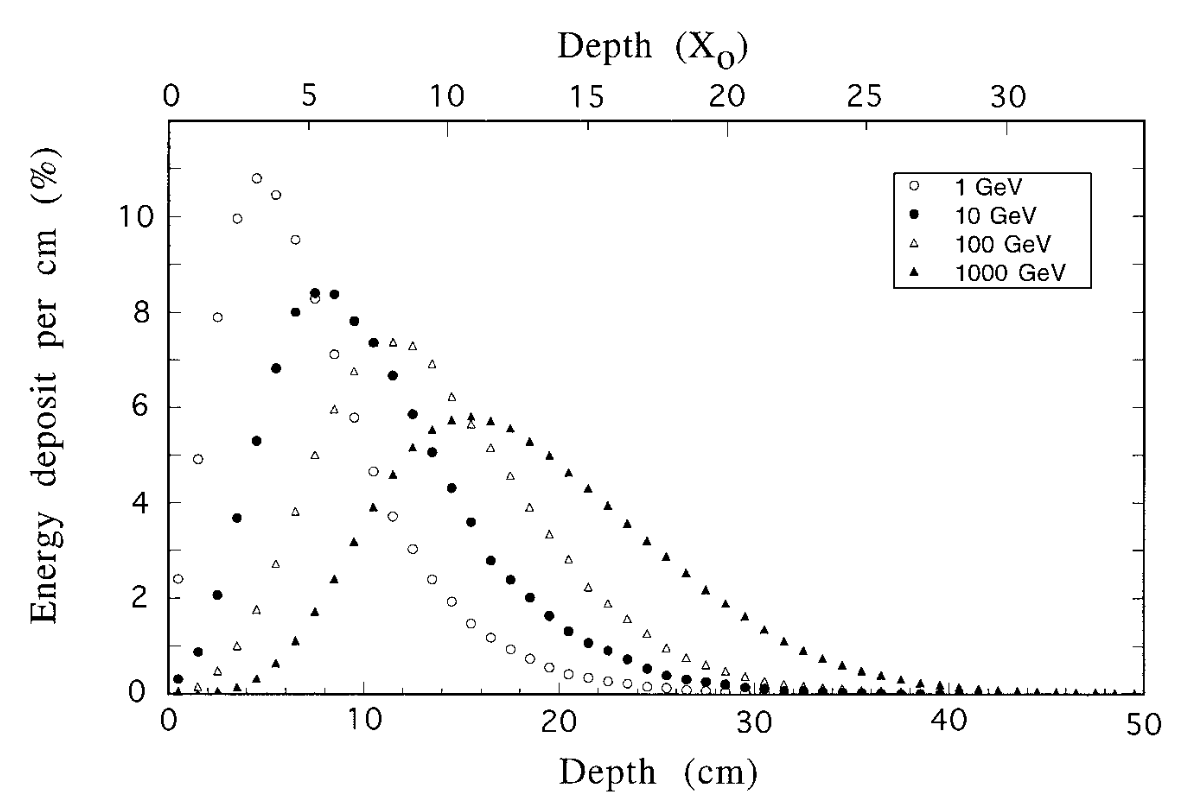
\includegraphics[width=0.7\textwidth]{IMG/Cap2/shower_max.png}
	\caption{The energy deposit as a function of depth, for $1$, $10$, $100$ and $1000\ GeV$ electron showers developing in a block of copper \cite{Leo}.}
	\label{fig:shower_max}
\end{figure}

Another quantity useful to describe the spatial shower development, in particular the transverse one, is the Molière radius. It is defined in terms of the radiation length and the critical energy:
\begin{equation}
    \rho_M = E_s \frac{X_0}{\varepsilon_c}
\end{equation}
where $E_s$ is defined as $m_c^2\sqrt{4\pi/\alpha} \simeq 21.2\ MeV$. This quantity is almost material-independent and, on average, a cylindrical volume with this radius around the shower axis contains $90\%$ of the shower energy. The lateral spread is mainly due to two effects: at high energy, electrons and positrons are moved away from the shower axis because of the deviation occurring in Compton scattering; photons and electrons are also produced in isotropic processes moving them away from the axis (spread more important in lower energy particles). Also brehemstralung process produces photons with a certain angle, contributing to the shower spread. Figure \ref{fig:shower_moliere} give an idea of the radial distribution of deposited energy.\\

\begin{figure}
	\centering
	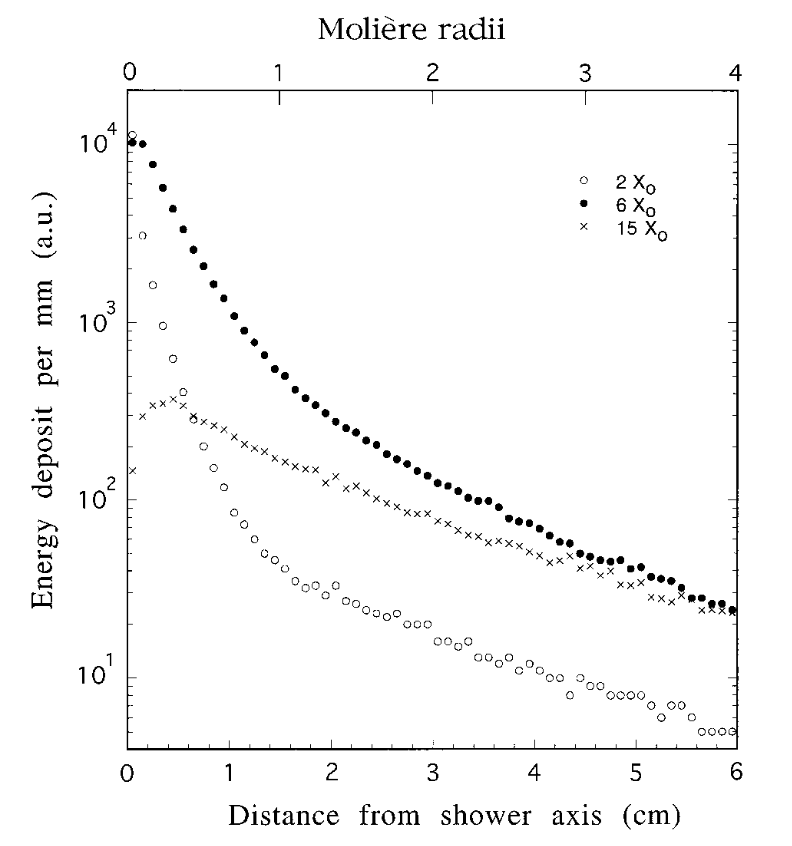
\includegraphics[width=0.6\textwidth]{IMG/Cap2/shower_moliere.png}
	\caption{The radial distributions of the energy deposited by $10\ GeV$ electron showers in copper, at various depths \cite{Leo}.}
	\label{fig:shower_moliere}
\end{figure}

The lateral and longitudinal shower development generated by charged particles and by neutral ones are basically identical except for the initial stages. Electrons start radiating as soon as they enter the calorimeter, instead photons must convert before releasing any energy. Once they start producing electrons and positrons, they can release even more energy than electron induced showers. This behaviour is shown in Figure  \ref{fig:em_start}, where the distribution of the energy fraction deposited in the first $5\ X_0$ by $10\ GeV$ electrons and photons in lead is plotted.

\begin{figure}
	\centering
	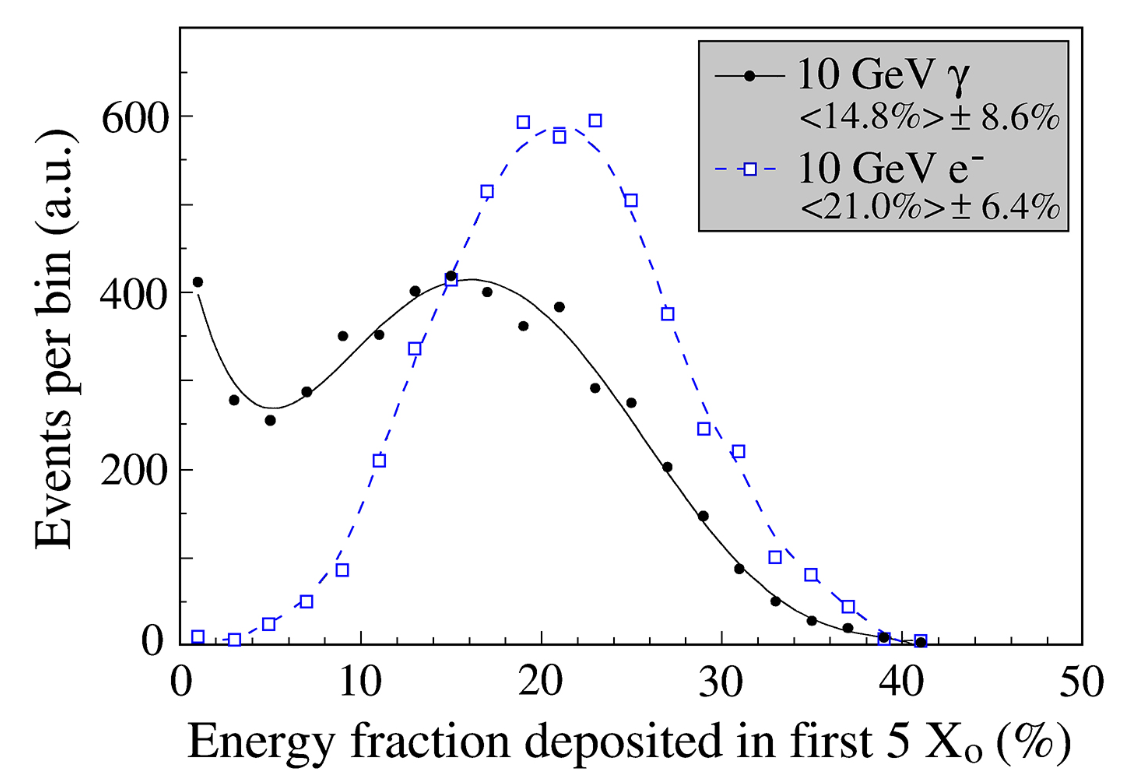
\includegraphics[width=0.7\textwidth]{IMG/Cap2/em_start.png}
	\caption{Distribution of the energy fraction deposited in the first $5\ X_0$ by  $10\ GeV$ electrons and photons showering in lead. Image from \cite{Wigmans_e_gamma}.}
	\label{fig:em_start}
\end{figure}

\subsection{Hadronic showers} \label{subsec:had_shower}
The hadronic showers, a new degree of complexity arises. The showers produced by hadrons are affected by the strong interaction. This interaction is responsible for:
\begin{itemize}
    \item The production of hadronic secondary particles, most of which, $\simeq 90\%$, are pions. Neutral pions mainly decay in two photons, which develop electromagnetic showers.
    \item The occurrence of nuclear reactions where atomic nuclei release neutrons and protons. The fraction of the shower energy needed to unbind the nucleons does not contribute to the energy released to the calorimeter (invisible energy phenomenon).
\end{itemize}
The part of energy released via electromagnetic showers is commonly named em fraction ($f_{em}$), and once the energy is converted to em showers it can not transformed back to hadronic energy. Another contribution to the complexity is given by the variability of this em fraction event by event and its energy dependence. On average, $f_{em}$ increases with the primary particle energy, since $\pi$s may also be produced by secondary and higher-order particles: the higher the energy,the more generations of shower particles, the larger em fraction. The  average  electromagnetic fraction has been evaluated to increase with the energy following the power law:
\begin{equation}
    f_{em} = 1 -1\left(\frac{E}{E_0}\right)^{k-1}
\end{equation}
where $K\simeq 0.82$ and $E_0$ is a matter dependent value of the order of $GeV$. The behaviour in lead and copper is shown in figure \ref{fig:f_em}.\\
In the calorimetry context, these characteristics have important consequences:
\begin{itemize}
    \item \textit{Non-compensation}; the calorimeter signals for hadrons and for electrons of the same energy are in general different a result of the invisible-energy phenomenon, in particular the one for hadrons is generally smaller.
    \item \textit{Non-linearity}; a calorimeter for hadron detection does not present a linear response with respect to the primary particle due tio the energy dependence of the em fraction.
\end{itemize}

\begin{figure}
	\centering
	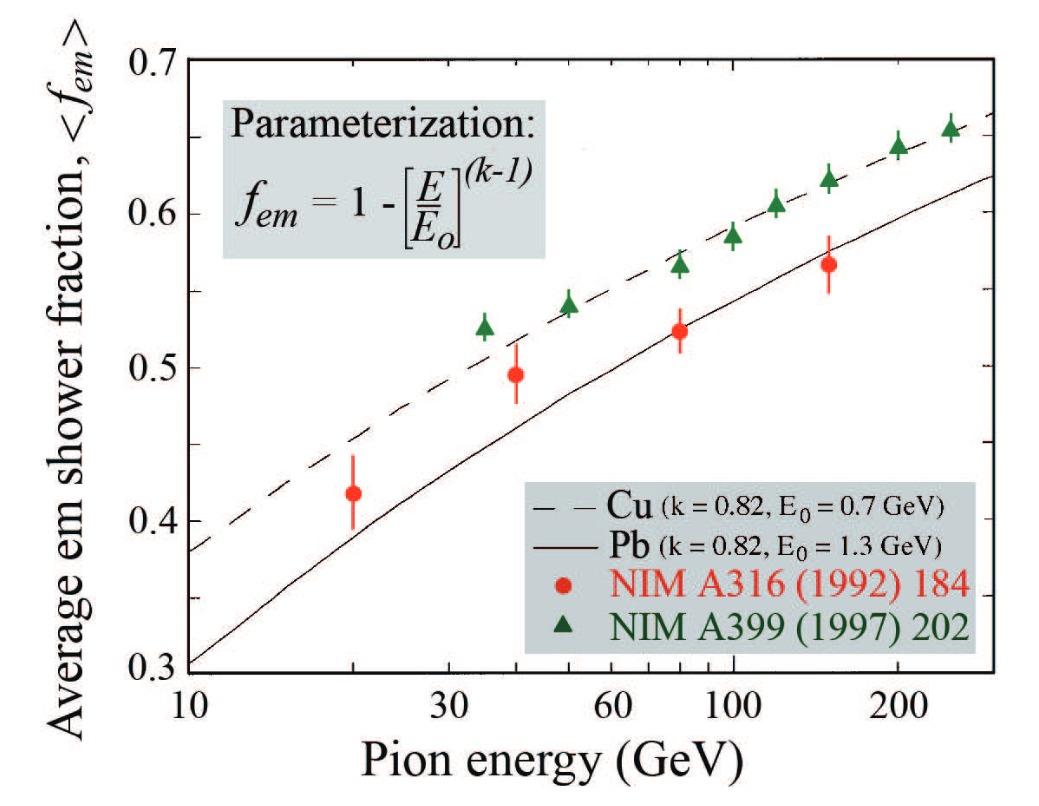
\includegraphics[width=0.7\textwidth]{IMG/Cap2/f_em.png}
	\caption{Comparison between the experimental results on the em fraction of pion-induced showers in copper-based and lead-based calorimeters. Image from \cite{Wigmans_e_gamma}.}
	\label{fig:f_em}
\end{figure}

Another important difference between em and hadronic showers is the greater spatial profiles of released energy. Analyzing for example several pions traces, peaks of signals are produced at a depth near the one where a $\pi^0$ is generated. However, the neutral pion production can occur in the second or third generation of the shower development releasing energy at different depth. An example of $4$ different showers from $270\ GeV$ pions is illustrated in figure \ref{fig:had_start}.\\
The depth of the calorimeter required to contain hadronic showers increases logarithmically with energy, as already seen for em showers, but the large longitudinal fluctuations make the leakage effect a point of extreme interest also in configuration that would contain, on average, $99\%$ of the shower.\\
Laterally, an hadronic shower is easier contained if the primary particle has higher energy. This is due to the fact that the electromagnetic shower fraction increases with energy. The em showers produced tend to develop laterally close to the shower axis.
 
 \begin{figure}
	\centering
	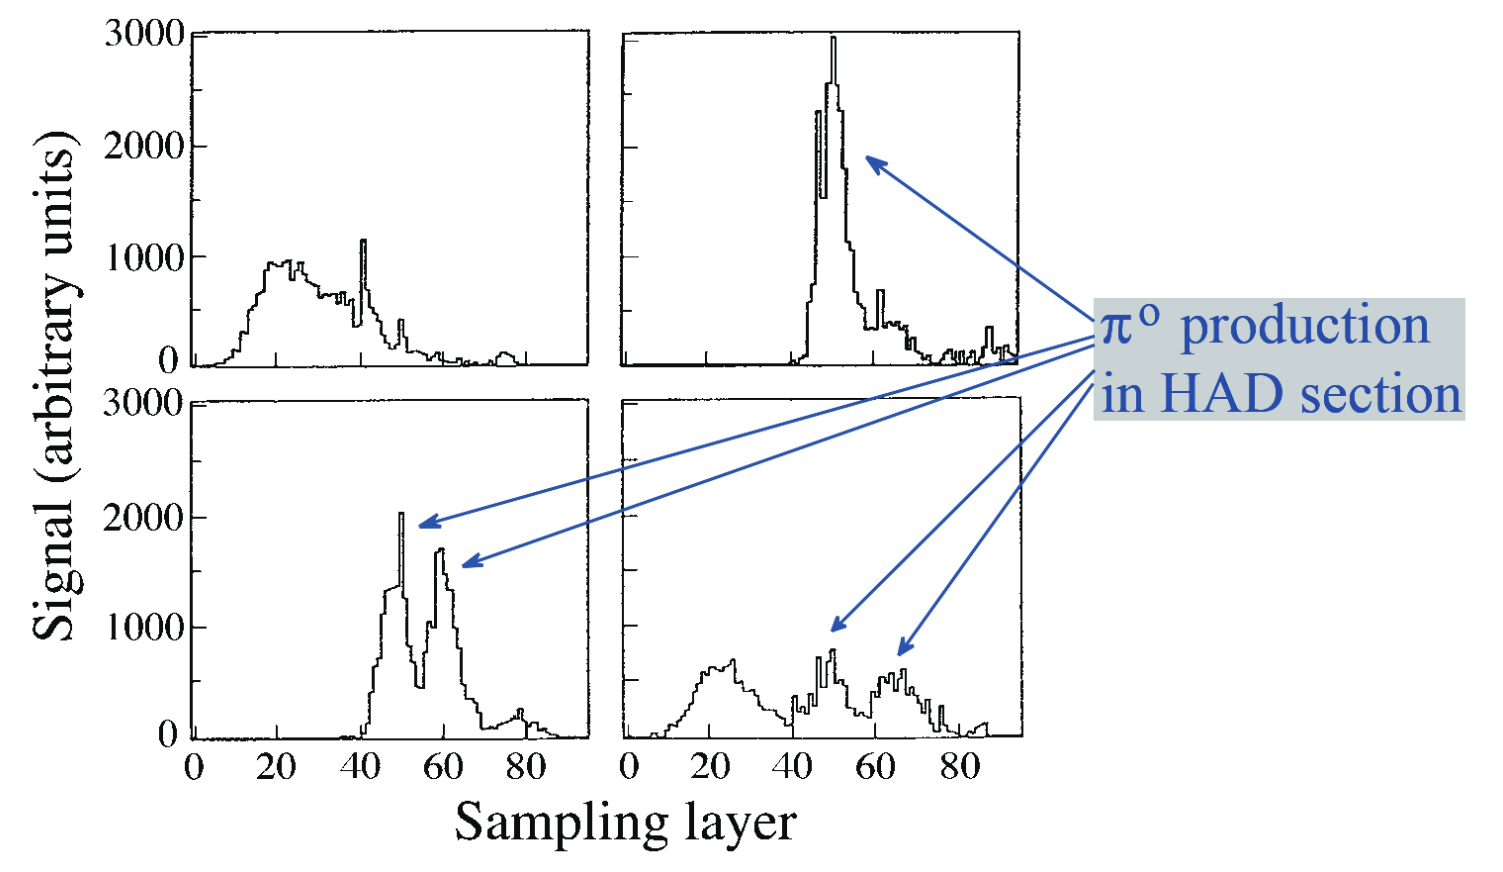
\includegraphics[width=0.7\textwidth]{IMG/Cap2/had_start.png}
	\caption{Longitudinal  profiles  for  $4$  different  showers  induced  by  $270\ GeV$  pions  in  a  lead/iron/plastic-scintillator calorimeter \cite{Wigmans_e_gamma}.}
	\label{fig:had_start}
\end{figure}

\section{Energy response of calorimeters}
Starting from the definition of the term \textit{response}, it is the average calorimeter signal per unit of deposited energy. The response is usually expressed in  terms, for example, of number of photoelectrons per $GeV$ or charge ($pC$) per  $MeV$. A straight forward definition is the linearity of a calorimeter, it is defined \textit{linear} if its response is constant.\\

\subsection*{Electromagnetic calorimeters}
Electromagnetic calorimeters are detector optimized to induce em showers. In these showers, all the energy carried by the primary particle is released by a very large number of shower particles through processes that may generate signals (excitation or ionization of the absorbing medium). The number of particles is on average proportional to the primary energy and the signal generated by each one of these is established by the detector properties. The direct consequence is that em calorimeters are in general linear detectors.\\
A non-linearity response is usually an indication of instrumental problems. The most common ones are:
\begin{itemize}
    \item leakage effects, caused by too small dimensions of the calorimeter;
    \item saturation effects of the active components, originated by possible high localized energy depositions;
    \item recombination of electrons and ions, making the energy carried by the electron undetected.
\end{itemize}

At the same time, the small lateral and longitudinal em shower development allows to design relatively small calorimeters, often used as electromagnetic components in more complex systems.\\

A structural distinction can be made between \textit{homogeneous} and \textit{sampling} calorimeter.\\
The main advantage of homogeneous detectors is their excellent energy resolution, achievable because the whole energy of the primary particle is released in the active medium. At the same time, if a well position measurement and particle identification are required, homogeneous calorimeters are not the best choice because of the challenging lateral and longitudinal segmentation task. 
Homogeneous calorimeter can be classified in four groups:
\begin{itemize}
    \item semiconductor calorimeters;
    \item Cherenkov calorimeters;
    \item scintillator calorimeters;
    \item noble-liquid calorimeters.
\end{itemize}

On the other hand, sampling calorimeters have in general worst energy resolution due to the presence of an absorber material (copper, iron, lead and uranium) that does not contribute to the signal and the sampling fluctuations. For electromagnetic sampling calorimeters, typical resolution values are in the range of $5-20 \% / \sqrt{E(GeV)}$. Meanwhile they are relatively simple to segment longitudinally and laterally due to their sampled structure contributing to achieve a better space resolution. Although this structure can be used to reduce the em calorimeter sizes, they are universally used in hadronic calorimeters.

\subsection*{Hadronic calorimeters}
Hadronic calorimeters are detector optimized to induce hadronic showers, are more complex because both em and hadronic shower are produced in them. The calorimeter response is, therefore, divided in em ($e$) and non-em ($h$) components. The ratio $e/h$ classifies calorimeters in three categories: \textit{compensating}, if $e/h=1$; \textit{undercompensating}, if $e/h>1$; \textit{overcompensating}, if $e/h<1$. Hence, the total calorimeter response (to charged pions) is a combination of the two:
\begin{equation}
    \pi = f_{em} \cdot e + (1- f_{em}) \cdot h.
\end{equation}
Since the average $f_{em}$ value, as already seen, increases with the energy, a non-compensating calorimeter response ($e/h \neq  1$) is not constant and hence non-compensating calorimeters are intrinsically non-linear detectors.
The $e/h$ value cannot be directly measured. However, it can be derived from the $e/\pi$ ratios, measured at various energies. The relationship between $e/\pi$ and $e/h$ is as follows, where $f_{em}$ is the energy dependent average em fraction:
\begin{equation}
    \frac{e}{\pi} = \frac{e/h}{1 - f_{em}(1-e/h)}
\end{equation}
The relation is represented in figure \ref{fig:compensation}.

 \begin{figure}
	\centering
	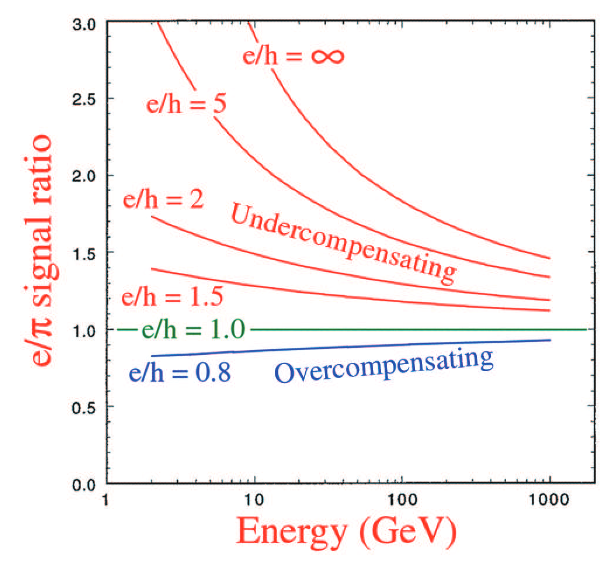
\includegraphics[width=0.65\textwidth]{IMG/Cap2/compensation.png}
	\caption{Relation between the calorimeter response ratio to em and non-em energy deposits, $e/h$, and the measured $e/\pi$ signal ratios \cite{Wigmans_e_gamma}.}
	\label{fig:compensation}
\end{figure}

The basic reason for different response for em and hadronic showers lies in the fact that in the absorption of hadronic showers, a significant fraction of the energy is \textit{invisible} not contributing to the calorimeter signal. The main source of this energy is the energy used to release nucleons from nuclei.\\
To design a linear calorimeter various compensation methods have been developed. There are two main approach to obtain $e/h = 1$: one is reducing the electromagnetic response and the other one is to increase the non-em response.\\
The most effective way to reduce the em response of a sampling calorimeter is to use as absorber an high-$Z$ material. The concept is based on the way that low energy photons release their energy. As seen, the main process at low energies is the photoelectric effect that is highly $Z$ dependent. For this reason, using high-$Z$ absorber materials causes an energy deposition in the absorber making this energy not detected.\\
The other strategy is known as compensation by neutrons signal boosting or by Signal Amplification through Neutron Detection (SAND). It consist in increasing the non-em response taking advantage of the kinetic energy transported by neutrons. The good correlation between the invisible energy and the kinetic energy of neurons opens the possibility of an event-by-event correction boosting the signals generated by the neurons. The most likely process to occur at low energies for a neutron is elastic scattering on a nucleus target. The fraction of energy transferred in this process is on average $f_{\text{elastic}} = 2A / (A +1)^2$ (where $A$ is the mass number of the target). Considering that hydrogen maximize this fraction it is the element that must be present in the active medium to produce the non-em response increment. With this consideration and fine tuning the sampling fraction, a $e/h$ ratio can be forced to be $1$ obtaining a linear hadronic calorimeter.
In short, compensation through SAND can be achieved in sampling calorimeters with active materials containing hydrogen and a precisely tuned sampling fraction.\\
In the IDEA dual-readout calorimeter, a more recent compensation strategy is designed. The dual-readout compensation used will be described in section \ref{sec:DRComp}.

\subsection{Fluctuations}
The energy response of a calorimeter represent an average value, but the energy loss is a statistical phenomenon therefore the precision of these detectors is affected and limited by fluctuations. The effect is quantified by the relative resolution defined energy distribution standard deviation divided by the mean value ($\sigma/E$).\\
Considering the simpler case of em calorimeters, four are the main sources of fluctuation:
\begin{itemize}
    \item sampling fluctuations;
    \item signal quantum fluctuations;
    \item shower leakage fluctuations;
    \item instrumental fluctuations.
\end{itemize}
Sampling effects are affected both by the sampling fraction (i.e. the ratio of the active material on the total) and the sampling frequency (the thickness of the layers). The sampling fraction is  defined as:
\begin{equation}
    f_{samp} = \frac{E_{active}}{E_{passive}+E_{active}}
\end{equation}
where $E_{active}$ and $E_{passive}$ are the energies deposited in the active and passive part by an incident minimum ionizing particle (mip).
This type of fluctuation is dominated by the Poisson statistics, hence it contribute with a term proportional to $1/\sqrt{E}$ to the energy resolution.
In em calorimeter with non-gaseous active material the sampling contribution follow the empirical law:
\begin{equation}
    \frac{\sigma}{E} = \frac{2.7\% \sqrt{d/f_{samp}}}{\sqrt{E}}
\end{equation}
where $d$ is the thickness of the active material layer measured in $mm$.\\
Under the label of signal quantum fluctuations are grouped fluctuation effects due, for example, to photon statistics in light emitting active materials. Also these fluctuations follow the rules of Poisson statistics, with the constrain of uncorrelated separate contributions. Another contribution that scales with $E^{-1/2}$ is added to the relative energy resolution expression.\\
In leakage fluctuations there are three possibilities: longitudinal, lateral and albedo. These fluctuation are highly dependent to the geometry and the material of the calorimeter. For this reason their contribution to the resolution does not have a precise energy dependent form. The typical solution to numerically evaluate their effect is to produce Monte Carlo simulation for the calorimeter and study the obtained data.\\
Finally, instrumental fluctuations are the ones provided, for example, by electronic noise or geometrical inhomogeneities. The electronic noise contribution is usually described with a term that scales with $1/E$ because it is largely independent of the shower energy. Meanwhile fluctuations induced by structural inhomogeneities depend on the shower position and might be energy dependent.\\
Typically, these contribution are uncorrelated and have to be added in quadrature to obtain the total resolution. As seen, different contribution with different energy dependence have to be considered. The consequence is that different effects dominate the energy resolution in different energy ranges. These behaviour have to be considered in the design of the calorimeter in order to optimize the resources.\\

All the sources described affect also hadronic calorimeters. For example, sampling fluctuation has a higher impact in hadronic showers due mainly to the lower average number of particle that release energy in the hadronic ones. 
At the same time, in hadronic detectors, resolution is affected also by other fluctuation effects.\\
The introduction of quantities such as $f_{em}$ in hadronic calorimeters produces new sources of fluctuations. In non-compensating calorimeter, event-by-event fluctuation in em component affect the detector response. It contributes to the relative energy resolution through a term scaling as $c E^{-0.28}$.
\begin{equation}
    \frac{\sigma}{E} = \frac{a_1}{\sqrt{E}} \oplus c E^{-0.28}
\end{equation}
Up to $400 GeV$, this law runs almost parallel to an energy resolution in which only the stochastic term is included ($\sigma/E = a/\sqrt{E}$). For this reason, the resolution of non-compensating calorimeter is described as:
\begin{equation}
    \frac{\sigma}{E} = \frac{a_2}{\sqrt{E}} + b.
\end{equation}l
A useful solution that bring remove these fluctuations is to design a compensating calorimeter, greatly improving the energy resolution.\\
Finally, the calorimeter resolution is also affected by invisible energy fluctuations. To evaluate the impact of these fluctuations the correlation between $f_{em}$ and $f_{inv}$ has to be known, and in particular if they are correlated or not. If they are uncorrelated the contribution to the resolution has to be added in quadrature. Moreover, in compensating calorimeter, the contribution of invisible energy fluctuations are different depending on the techniques used to achieve compensation.

\section{Dual-readout compensation}\label{sec:DRComp}
All the benefits obtained with compensating calorimeters are obtaining by sampling em and non-em components in hadronic showers with the same response ($e=h$). Dual-readout is a method that perform this correction event-by-event, constantly measuring the electromagnetic fraction [cite?]. 

\subsection{Working principles}
This technique is based on the concept that the em component is mostly provided by relativistic electrons and positrons, while the majority of non-em one is carried by non-relativistic particles. Hence, collecting the Cherenkov signal produced by an hadronic shower is almost equivalent to sampling the em component, estimating the electromagnetic fraction. A second simultaneous signal, typically from scintillators, is recorded. Thanks to this second signal, the non-em component can be evaluated starting from the $f_{em}$ already obtained.\\

Entering the details of the process, let's consider scintillation (S) and Cherenkov (C) signals produced by an hadronic shower. The mean values of these signals are calibrated with an electron beam of known energy $E$ so that, for em showers, $\expval{S} = \expval{C} = E$. The hadronic signals can be written (for each event) as:
\begin{align}
    S &= E \left[f_{em} + (h/e)_S (1-f_{em}) \right], \label{eq:S} \\
    C &= E \left[f_{em} + (h/e)_C (1-f_{em}) \right], \label{eq:C}
\end{align}
where $h/e$ quantify the two different degree of non-compensation for the two signals. Considering that $h/e$ are measurable quantities and are assumed to be constants, the ratio $C/S$ is also energy independent:
\begin{equation}
    \frac{S}{C} = \frac{f_{em} + (h/e)_S (1-f_{em})}{f_{em} + (h/e)_C. (1-f_{em})} \label{eq:em_frac}
\end{equation}
This expression can straightforwardly give an evaluation of the em fraction:
\begin{equation}
    f_{em} = \frac{(h/e)_C-(C/S)(h/e)_S}{(C/S)\left[1-(h/e)_S\right]-\left[1-(h/e)_C\right]}
\end{equation}
allowing the rewriting of \ref{eq:S} and \ref{eq:C} as
\begin{align}
    S/E &= (h/e)_S + f_{em}\left[1-(h/e)_S\right], \label{eq:S2} \\
    C/E &= (h/e)_C + f_{em}\left[1-(h/e)_C\right]. \label{eq:C2}
\end{align}

A $C/E$ vs $S/E$ scatter plot can be sketched using signals from a generic DR calorimeter for electrons, pions and protons showers. An example is shown in figure \ref{fig:theta_DR}. As expected, data generated from electrons are always around the point $[1,1]$ (where $f_{em} = 1$). On the other hand an hypothetical signals with only non-em component would be at $[(h/e)_S,(h/e)_C]$ where $f_{em}$ is $0$. Signals from pions and protons showers are clustered along a straight line linking these two points. From this geometric construction it is clear that the slope of this line (the $\theta$ angle) is energy independent because it is determined only by the two $e/h$ values. Thanks to the fact that $\theta$ is energy and particle independent, it is possible to define the parameter:
\begin{equation}
    \chi = \frac{1-(h/e)_S}{1-(h/e)_C} = \cot{\theta},
\end{equation}
this parameter can also easily estimated with test beam data depending only on calorimeter material and geometry.
Finally, event-by-event, the energy of each hadron shower can reconstructed  using the $S$ and $C$ signals in an unique way:
\begin{equation}
    E = \frac{S - \chi C}{1 - \chi}.
\end{equation}

\begin{figure}
	\centering
	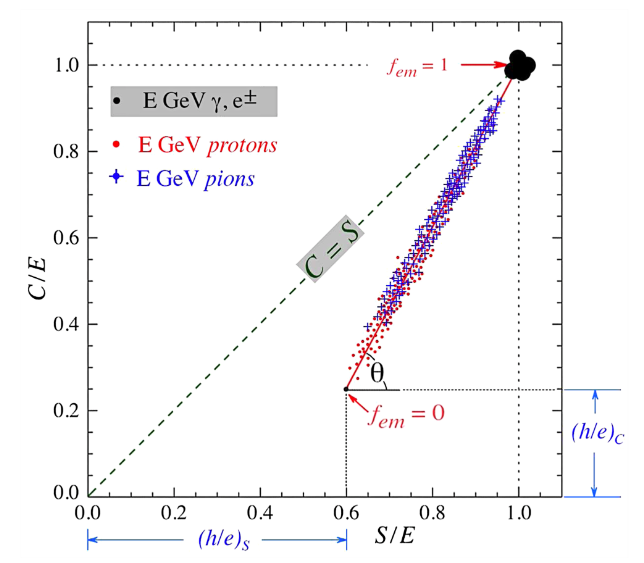
\includegraphics[width=0.65\textwidth]{IMG/Cap2/theta_DR.png}
	\caption{Relation between the calorimeter response ratio to em and non-em energy deposits, $e/h$, and the measured $e/\pi$ signal ratios \cite{Wigmans_e_gamma}.}
	\label{fig:theta_DR}
\end{figure}

The ideal DR calorimeter is able to identify the Cherenkov signal as the exact electromagnetic component ($h/e = 0$) being a direct measurement of $f_{em}$. The worst DR calorimeter instead is designed when $(h/e)_C = (h/e)_S$, in this case the two signals would sample the two components (em and non-em) with the same response giving no information about the $f_{em}$ from the $S/C$ ratio.  Therefore, the best real DR calorimeter is the one with the lower $\chi$ parameter found with the lower $(h/e)_C$ and the higher $(h/e)_S$ values possible. 

\subsection{Experiments}
At present a few dual-readout calorimeter have been built and tested, and more project are under study.\\
The first practical usefulness of the dual-readout method was tested in a R&D study for the Advanced Cosmic Composition Experiment at the Space Station (ACCESS) cite?. The prototype had a depth of $1.4\lambda_{int}$ and was equipped with both plastic-scintillator ($S$) and quartz ($Q$) optical fibres to measure and collect the scintillation and Cherenkov light, respectively. With this detector, the $Q/S$ signals ratio was found to represent a good event-by-event measurement of the shower energy fraction carried by $\pi^0$.\\
Later, a $10 \lambda_{int}$ deep calorimeter known as Dual-REAdout Method (DREAM) was built and tested. 
The detector is composed by $5580$ basic element represented in figure \ref{fig:DREAM}. These are $200\ cm$ long, hollow, extruded copper rod of $4\times 4 mm^2$ cross section in which $3$ scintillating and $4$ Cherenkov fibres are inserted.
\begin{figure}
	\centering
	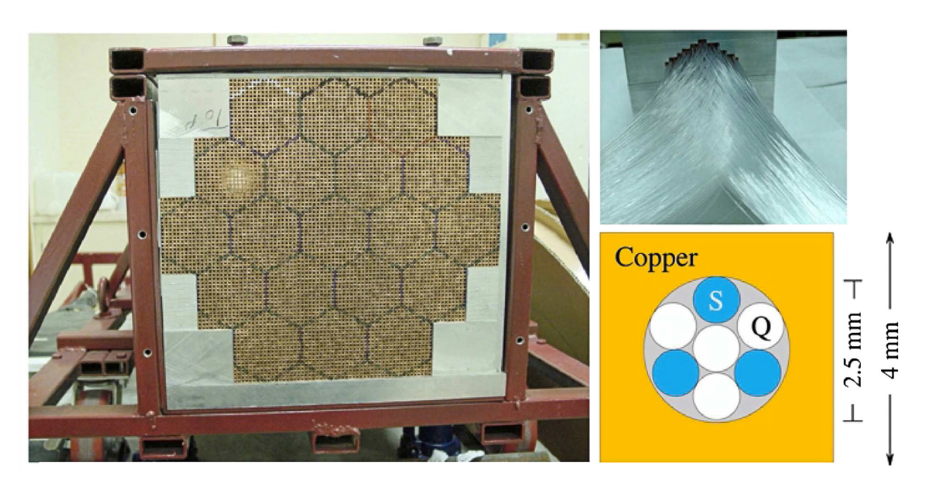
\includegraphics[width=0.65\textwidth]{IMG/Cap2/DREAM.png}
	\caption{The DREAM calorimeter layout cite?.}
	\label{fig:DREAM}
\end{figure}

Figure \ref{fig:theta_DREAM} shows the $C-S$ scatter plot of the calibrated signals, where the correlation between them its clear.
The two $h/e$ ratios for Cherenkov and scintillator DREAM structures are $0.21$ and $0.77$, respectively. The expression of the em fraction \ref{eq:em_frac} becomes:
%\begin{equation}
%    \frac{C}{S} = \frac{f_{em} + 0.12 (1-f_{em})}{f_{em} + 0.77 (1-f_{em})}.
%\end{equation}
\begin{equation}
    f_{em} = \frac{0.21-0.77(C/S)}{(C/S)\left[1-0.77\right]-\left[1-0.21\right]}
\end{equation}

\begin{figure}
	\centering
	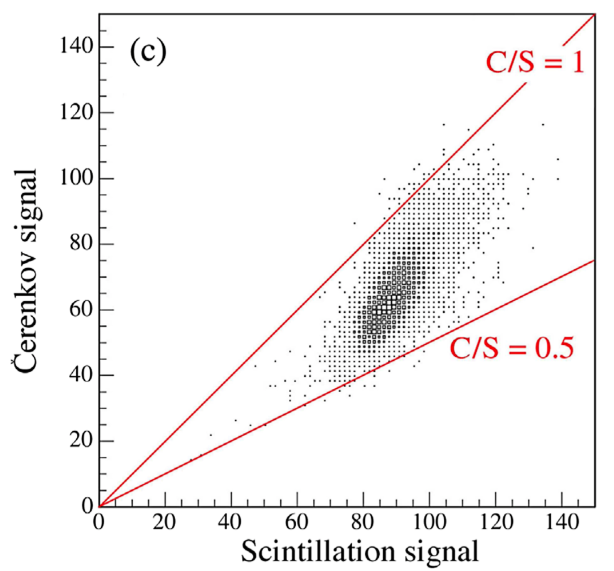
\includegraphics[width=0.65\textwidth]{IMG/Cap2/theta_DREAM.png}
	\caption{ The $C−S$ scatter plot showing the correlation between both types of signals. The signals are expressed in the same units used to calibrate the calorimeter (em GeV) cite?.}
	\label{fig:theta_DREAM}
\end{figure}

The DREAM results, together with other studies (e.g. SPACAL and RD52) confirmed the potentiality and the good concept of the dual-readout compensation method, bringing to the IDEA dual-readout calorimetry project.
		
		%--------CAPITOLO 3--------
		\chapter{Calorimetry and dual-readout}
Calorimetry is an important detection principle in particle physics.
Originally developed with astrophysical purpose for cosmic-ray studies, this method refers to the detection of particles and the measurement of their properties, using blocks of instrumented material.
It was developed and perfected for accelerator-based particle physics experimentation primarily in order to measure the energy of particles. 
In these blocks, particles are fully absorbed and their energy transformed into a measurable quantity.\\
The incident particle interact with the detector (through electromagnetic or strong processes) producing a shower of secondary particles with progressively degraded energy.
The energy deposited by the charged particles of the shower in the active material of the calorimeter, which can be detected in the form of charge or light, is used to measure the energy of the incident particle.
Typical processes suitable to detect this energy are: ionization of the medium, scintillation light and the Cherenkov light produced by relativistic particles.\\

Calorimeters can be divided into two categories depending on the type of shower they are optimized to detect: electromagnetic calorimeters, used mainly to measure electrons and photons through their electromagnetic interactions (e.g., bremsstrahlung, pair production), and hadronic calorimeters, used to measure mainly hadrons through their strong and electromagnetic interactions.\\
Another classification can be made according to their construction technique defining sampling calorimeters and homogeneous calorimeters.\\
Homogeneous calorimeters are built of one type of material that performs both the main tasks: degrade the energy of the incident particles and provide the detectable signal.\\
Sampling calorimeters, instead, consist of alternating layers of an absorber, a dense material used to perform energy degradation, and an active medium that generate the signal.\\

%Calorimeters are attractive in high-energy particle physic field for various reasons:
%\begin{itemize}
%		\item In most cases the calorimeter energy resolution improves with energy as $1/\sqrt{E}$, where $E$ is the energy of the incident particle. Therefore calorimeters are very well suited to high-energy physics experiments.
%		\item Calorimeters are sensitive to all types of particles, charged and neutral (e.g., neutrons). Also neutrinos and their energy can be indirectly detected can even provide indirect detection of neutrinos and their energy through the measurement of the event missing energy.
%		\item They are versatile detectors. They can be used to determine the shower position and direction, to perform particle identification, to measure the arrival time of the particle, or even to provide fast signals useful in trigger purpose.
%		\item They are space and therefore cost effective. Because the shower length increases only logarithmically with energy, the detector thickness needs to increase only logarithmically with the energy of the particles.
%\end{itemize}

This chapter describes the physics behind both the electromagnetic and hadronic shower developments, provides a basic description of the energy response of these detectors and introduces the particular technique of the dual-readout, a modern concept of calorimeter that has the quality of overcome the non-compensating problem measuring both electromagnetic and hadronic showers through two different type of signals simultaneously (Cherenkov and scintillation light).\\

\section{Physics of shower development}
A particle interact and lose part or whole of its energy traversing matter. During this process the medium get excited and heated up, is excited in this process, or heated up. From this feature the term calorimetry, litteraly meaning "heat mesurement", was introduced.\\
The groundwork for the calorimetry is the interaction processes between particle and matter. They are the manifestation of the electromagnetic, the strong and, more rarely, the weak forces and they strongly depend on the energy and the nature of the incident particle, in addition to medium features.\\
The processes and the consequent shower effects are the keys to deeply understand this topic.\\

\subsection{Electromagnetic showers}
aaa

\subsection{Hadronic showers}
aaa

\section{Energy response of calorimeters}
aaa

\subsection{Homogeneous calorimeters}
aaa

\subsection{Sampling calorimeters}
aaa

\subsection{Compensation}
aaa

\section{Dual-readout calorimetry}
aaa

\subsection{Working principles}
aaa

\subsection{Experiments}
		
		%--------CAPITOLO 4--------
		\chapter{IDEA DR calorimeter full simulation}
As already said, the concept described in chapter \ref{chap:Idea_project} is an on-going project and it has to be supported by simulation.
With this goal, a dual-readout calorimeter full simulation has been developed allowing to generate data and monitor the whole process from the collision on the interaction point to the digitized signal produced by SiPMs.\\

The chapter presents a description of the simulation structure. The section \ref{sec:Sim_struc} describes in details the simulation dividing it in two main Monte Carlo processes:
\begin{itemize}
	\item the calorimeter simulation, coded in GEANT4;
	\item the SiPM response digitization (``pySIPM"), coded in Python.
\end{itemize}

Later, the performances obtained will be shown. The temporal behavior, the SiPM saturation effect and the energy resolution will be described in section \ref{sec:Sim_perf}.\\

Then the chapter treats of the possibility of simple particle identification using neural network structures.\\
%In section \ref{sec:NN_waveform} neural networks working on digitized waveforms are described. The aim of these neural network is to correctly distinguish waveforms generated by electrons ($e^-$) or pions ($\pi^-$) in a range of energy from $20$ to $80$ GeV.\\
The last section (sec.\ref{sec:NN_img})  exposes a neural network that has the purpose of identify if signal are generated from photons ($\gamma$) or neutral pions ($\pi^0$). This aim is achieved analyzing the spatial pattern of energy released in the calorimeter.

\section{Simulation structure} \label{sec:Sim_struc}

\subsection{Calorimeter simulation} \label{subsec:Sim_cal}
The calorimeter simulated follows the idea show in chapter \ref{chap:Idea_project}. It has a cylindrical symmetry characterized by a barrel and two endcaps. This $4\pi$ structure is obtained rotating $36$ simpler component, called slices, around the $z$ axis. The dimensions of the slices are shown in figure \ref{fig:cal_slices}, therefore the inner diameter and  the inner length are both $5\ m$ meanwhile the overall outer diameter and length are $9\ m$.\\
Each half slice is composed by 75 $2\ m$ long towers ($40$ part of the barrel and $35$ part of the endcap), $5400$ of this element are used to set up the whole calorimeter.
To correctly cover an almost $4\pi$ solid angle each tower has different trapezoidal inner face with dimensions that can vary from $\sim 5\ cm$ to $\sim 8\ cm$.
A small circular area, with $0.25\ m$ of radius, centered along the $z$ axis is not covered by the calorimeter to permit the beam to reach the interaction point (IP).\\

%\begin{figure}
%	\centering
%	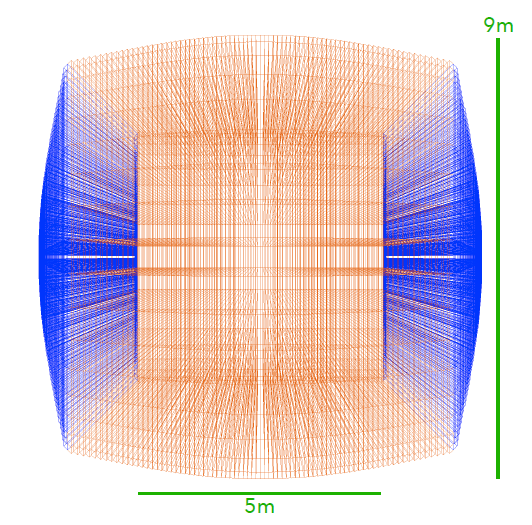
\includegraphics[width=0.6\textwidth]{IMG/DRCGeometry3}
%	\caption{Calorimeter geometry.}
%	\label{fig:cal_geometry}
%\end{figure}
\begin{figure}
	\centering
	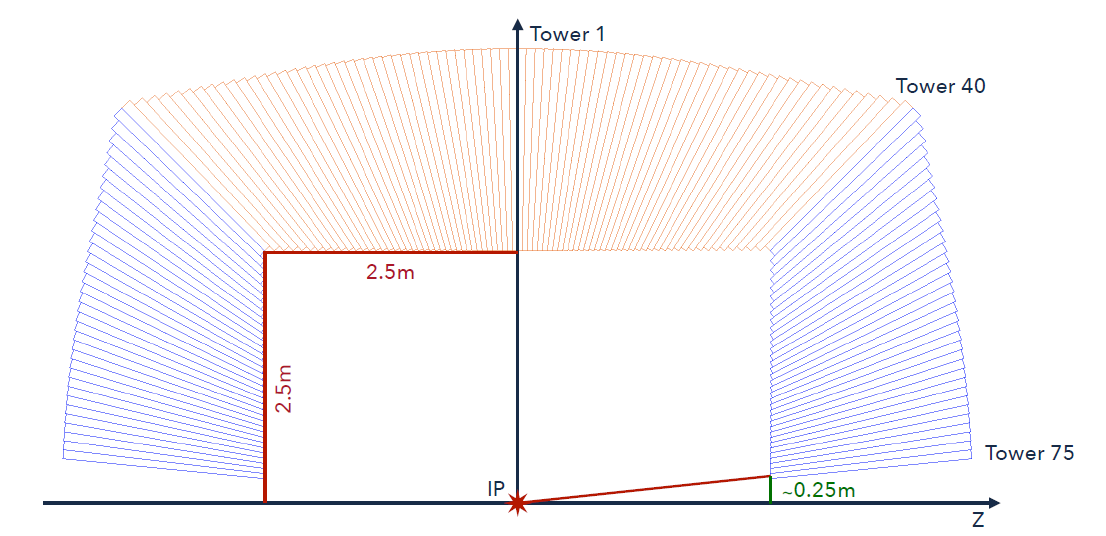
\includegraphics[width=0.8\textwidth]{IMG/DRCGeometry1}
	\caption{Calorimeter single slice.}
	\label{fig:cal_slices}
\end{figure}

The towers are copper based and play the role of absorber. To have a sensitive element they are filled by optical fibres. The idea of a projective calorimeter make the absorber volume greater increasing the distances from the IP. New fibres at different depth have to be placed inside the calorimeter to keep constant the sampling fraction.\\
As the dual-readout technique needs to distinguish Scintillating ($S$) and Cherenkov ($C$) signal, two types of fibres are used (fig. \ref{fig:CS_fibres}). Their characteristic are shown in tab. \ref{tab:fibres}.\\
The fibre refractive indices determine the light transport (as consequence of the Snell's law \cite{Snell}). The signal from the scintillating fibres is parametrised by the deposited energy while the Cherenkov photons are produced accordingly to the Cherenkov emission process.\\

\begin{table}
	\centering
	\setlength{\tabcolsep}{12pt}
	\begin{tabular}{lp{0.6\textwidth}}
		\toprule
		\multicolumn{2}{c}{\textbf{Kuraray SCSF-78 ($S$)}}	\\
		\midrule
		Core:				& $r = 0.485\ mm$, Polystyrene ($C_5H_5$), $\rho=1.95\ g/cm^3$, $n = 1.59$	\\
		Cladding: 			& Thickness $=2\%$ of $r$, PMMA ($C_5H_8o_2$), $\rho=1.19\ g/cm^3$, $n=1.49$	\\
		Main properties:	& Emission constant $= 2.8\ ns$, LY $= 10^4\ \text{photons}/MeV$, $\lambda_{att} = 4\ m$	\\
		\midrule
		\multicolumn{2}{c}{\textbf{Mitsubishi SK-40 ($C$)}}	\\
		\midrule
		Core:				& $r = 0.485\ mm$, PMMA ($C_5H_8o_2$), $\rho=1.19\ g/cm^3$, $n = 1.49$	\\
		Cladding: 			& Thickness $=2\%$ of $r$, Fluorinated Polymer ($C_2F_2$), $\rho=1.43\ g/cm^3$, $n=1.42$	\\
		Main properties:	& $\lambda_{att} = 8.9\ m$	\\
		\bottomrule
	\end{tabular}
	\caption{Technical characteristics of the two type of fibres used.}
	\label{tab:fibres}
\end{table}

\begin{figure}
	\centering
	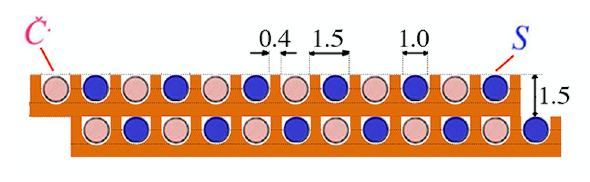
\includegraphics[width=0.8\textwidth]{IMG/DRCGeometry2}
	\caption{Chess-like configuration to dispose the fibres in the copper structure.}
	\label{fig:CS_fibres}
\end{figure}

For each event, the simulation gives as output useful information: 
\begin{itemize}
	\item Event ID;
	\item Fibre Type;
	\item Fibre ID;
	\item the position of the fibre end closer to the IP;
	\item the number of photons reaching the fibre further end;
	\item the list of photons time of arrival to the fibre end.
\end{itemize}

The computation of light propagation is extremely time consuming, so that it has to be fine tuned to optimize the process. In particular, the propagation of $C$ photons is tracked until the single photon reach the core-cladding boundary (i.e. at the distance $R$ from the further end of the fibre and at the time $t_0$). If the emission angle is inside the range of the fibre numerical aperture, the photon is added to the final number of photons (after a Poissonian smearing on their number).
The time of arrival on the sensor for each photon is estimated as:
\begin{equation}
t_C = t_0 + R \frac{n_C}{c}
\end{equation}
where $n_C = 1.49$ is the fibre refractive index and $c$ is the speed of light.\\

The $S$ fibres, instead, carry scintillating photons produced considering the light yield of the fibres and the energy deposited by the interacting particle. The number of photons is smeared with as Poissonian law and de time of arrival on the sensor is obtained as:
\begin{equation}
	t_S = t_0 + R\frac{n_S}{c\cdot \cos(\vartheta)} + t^*
\end{equation}
where $n_S = 1.59$ is the refractive index and $t^*$ is a random time that considers the fibres decay time, it is chosen from an exponential distribution with $2.8\ ns$ as mean value.
Considering the internal reflection, the photon path depends on the $\vartheta$ angle (i.e. the angle between the photon direction and the fibre axis). It is chosen randomly in the range $[\cos(\alpha),\cos(0)]$, where $\alpha = 20.4\degree$ is the fibre critical angle.\\
Eventually, the light produced is smeared by two Poissonian distribution, one for scintillation photo-electrons and the other one for Cherenkov photo-electrons. This procedure correctly reproduces statistic fluctuations in scintillation and Cherenkov light production and allows to reproduce within simulations the scintillating light yield (p.e./GeV) desired. To make the full simulation lighter, this process also includes the attenuation due to the PDE of the simulated SiPMs. The simulation is tuned to produce $\sim 400\ Spe/GeV$ and $\sim 100\ Cpe/GeV$ at the electromagnetic scale.

\subsection{SiPM response digitization} \label{subsec:Sim_SiPM}
The results obtained are the input of the second part of the simulation: \textit{pySiPM}, a Monte Carlo simulation, performed mostly in Python, able to reproduce the SiPM response to a light source and replicate the waveforms recorded with a digitizer \cite{digitizer}.\\

The importance of this software goes beyond our context, but perfectly fits our needs. In particular each fibre from the calorimeter simulation is considered coupled to a single SiPM, which digitized response is simulated through \textit{pySiPM}.

The simulation allows to set most of the SiPM parameters:
\begin{itemize}
	\item \textbf{Geometrical parameters}: the sensor dimensions and the pixel pitch.
	\item \textbf{Sensor parameters}: Photon Detection Efficiency, Dark Count Rate, After-Pulse probability, Optical Cross-Talk probability.
	\item \textbf{Signal parameters}: rise time constant, decay time constant.
	\item \textbf{Waveform parameters}: time window, sampling time, integration window.
\end{itemize}

For each event and fibre, random parameters determine the photon position inside the sensor. %Meanwhile the sensor PDE is tuned to have consistent mean values of $\sim 400\ Spe/GeV$ and $\sim 100\ Cpe/GeV$ respectively for $S$ and $C$ light yield.
Meanwhile the sensor PDE is set at $100\%$ to be consistent with the smearing applied at the calorimeter simulation level.
A control stop the count of impinging photons on the same cell to a maximum one, then each element of noise is generated with the set probability.\\
The pulse generated is a combination of two exponentials characterized by the rise time constant ($\tau_{rise}$) and the decay time constant ($\tau_{fall}$), considering the different photon time of arrival ($t_S$ and $t_C$):
\begin{equation}
	y(t)= A \cdot \left( e^{-\frac{t}{\tau_{fall}}} - e^{-\frac{t}{\tau_{rise}}}\right).
	\label{form:resp_func}
\end{equation}

The total signal of each SiPM is the sum of all the signals generated from the activated cells.\\

The information given as output of the simulation are:
\begin{itemize}
	\item \textbf{Data reported from GEANT4 simulation}: event ID, type of fibre, fibre ID, fibre position;
	\item \textbf{Computated quantities}: integral, peak height, time of arrival, time over threshold, time of peak;
	\item \textbf{Digitized waveform}.
\end{itemize}

All this features can be rejected through a trigger, in particular a threshold can be set to establish the informations that have to be recorded.
The threshold is defined as a scale of the maximum value of a waveform generated by a single photoelectron (neglecting the electrical noise). In the results showed later a one-suppression has been applied using a threshold factor of $1.5$, a typical setup to filter isolated signals of DCR.\\

\section{Simulation performances} \label{sec:Sim_perf}

\subsection{Different configurations} \label{subsec:SiPM_conf}
The results shown in this last chapter are obtained considering different SiPM parameters configurations.\\
They have been chosen in a common parameter space identified checking the lineup of SiPMs produced by Hamamatsu \cite{SiPM_lineup}. 
Two are the parameters that has been changed in our studies: 
\begin{itemize}
	\item the decay time constant of the signal, the chosen values are $10\ ns$ and $50\ ns$;
	\item the pixel size, the chosen values are $10\ \mu m$, $15\ \mu m$ and $25\ \mu m$.
\end{itemize}

The other fixed values of parameters are listed in the table \ref{tab:SiPM_par}.\\

\begin{table}
	\centering
	\setlength{\tabcolsep}{18pt}
	\begin{tabular}{ll}
		\toprule
		\multicolumn{2}{c}{\textbf{Geometrical Parameter}}	\\
		SiPM area	& $1 \times 1\ mm^2$	\\
		\midrule
		\multicolumn{2}{c}{\textbf{Sensor Parameters}}	\\
		DCR			& $200 \ kHz$	\\
		After-Pulse	& $3\% $	\\
		Cross-Talk	& $1\% $	\\
		\midrule
		\multicolumn{2}{c}{\textbf{Signal Parameter}}	\\
		Rise time	& $1\ ns$	\\
		\midrule
		\multicolumn{2}{c}{\textbf{Waveform Parameters}}	\\
		Time window	& $500 \ ns$	\\
		Integration window	& $300 \ ns$	\\
		Sampling frequency	& $10\ GHz$	\\
		\bottomrule
	\end{tabular}
	\caption{Fixed SiPM parameters used in the simulation configuration file. To know also variable parameters see text.}
	\label{tab:SiPM_par}
\end{table}

An example of waveform generated is plotted in figure \ref{fig:diff_wf} where is clear the difference produced using two different decay time constant.

\begin{figure}
	\centering
	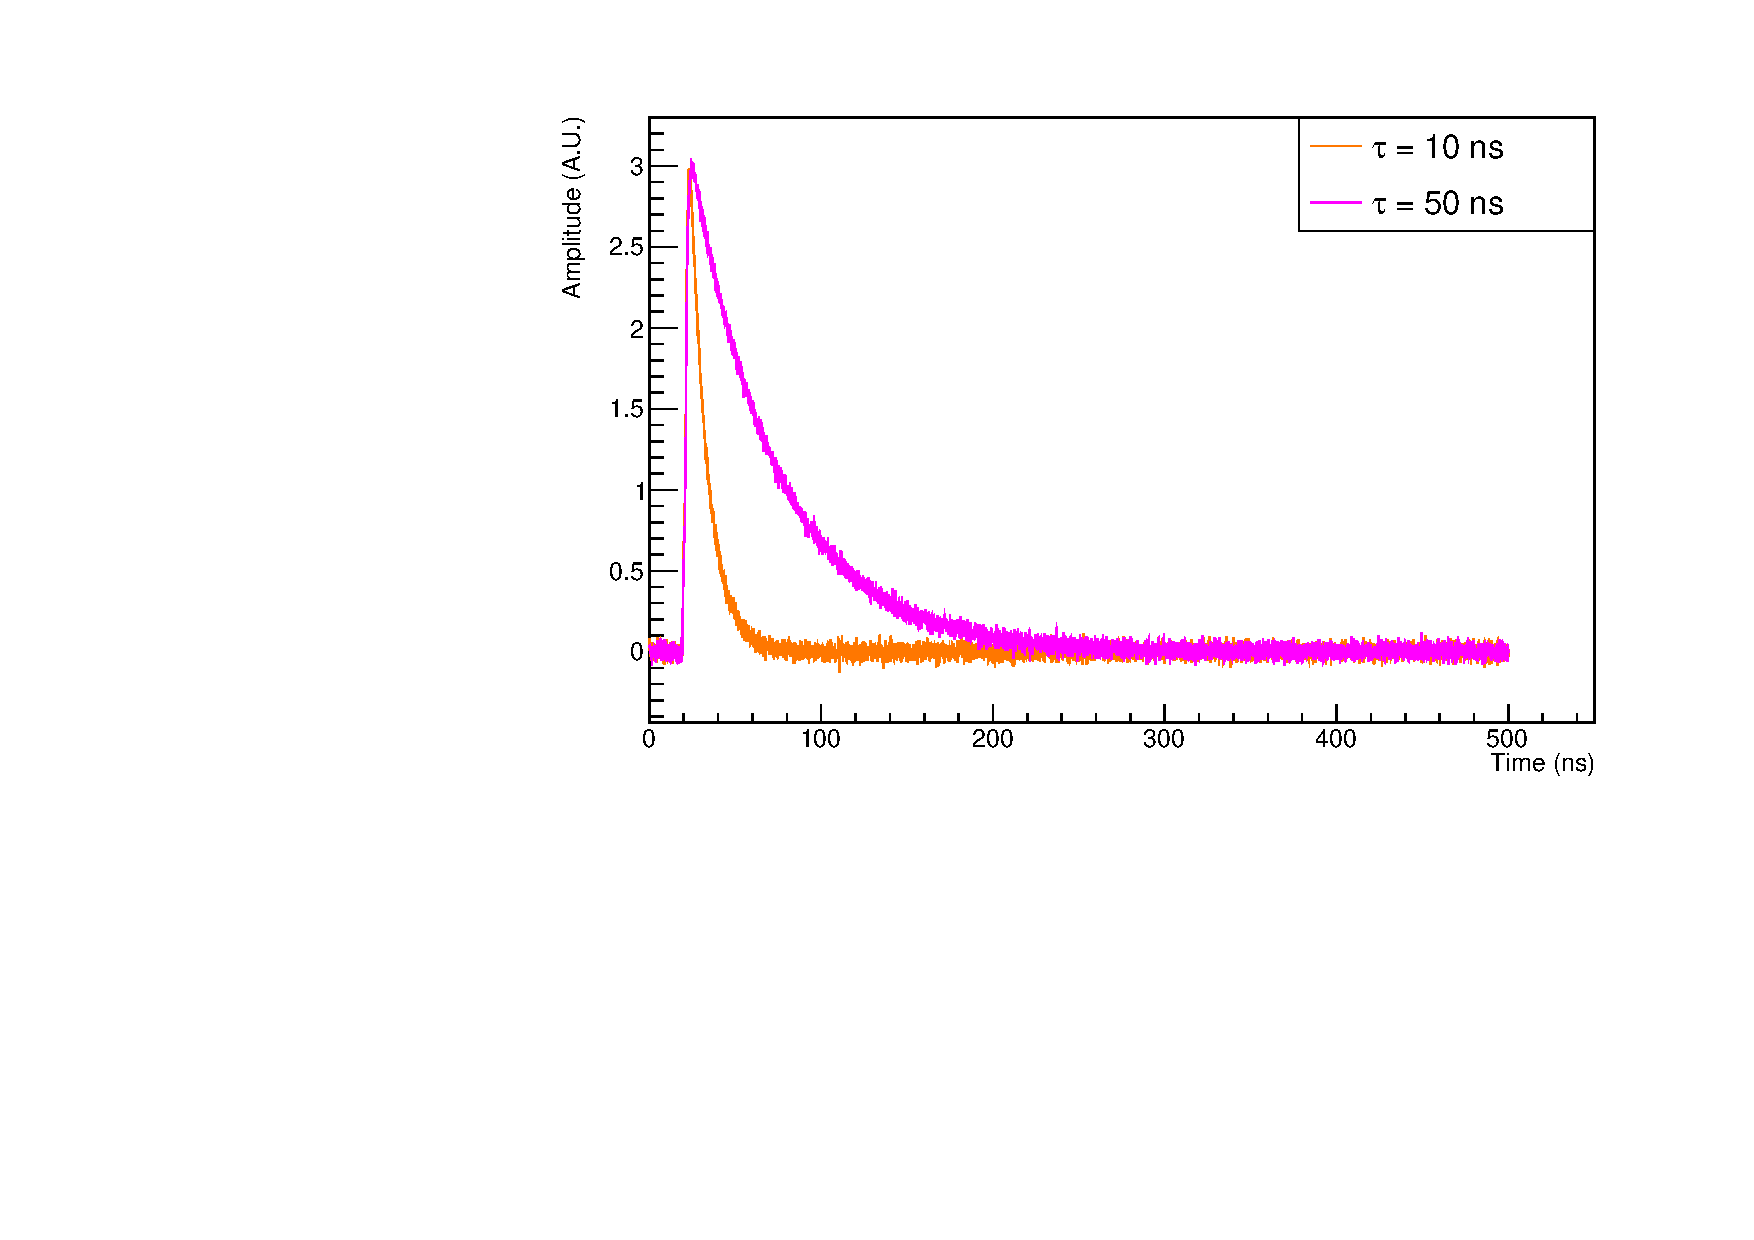
\includegraphics[width=0.8\textwidth]{IMG/Cap5/wf_different_conf}
	\caption{Single waveforms generated in two identical condition except for the decay time constant in the SiPM configuration file.}
	\label{fig:diff_wf}
\end{figure}

\subsection{Time studies} \label{subsec:Time}
An important aspect that has to be studied is the temporal one.
In order to do this, data of $1000$ events are produced. In each event a $20\ GeV$ electron is produced from the interaction point.\\
A first step is to analyze the distribution of the time of arrival of the photons converted at the SiPMs (i.e. the time recorded in the GEANT4 simulation output).\\
The distribution obtained from $C$ and $S$ photons are plotted in figure \ref{fig:true_toa_dist}.
As expected, the distribution of $C$ photons time extremely narrow due to the instantaneous production of photons at the passage of relativistic charged particle in the fibres, instead the $S$ photons time distribution shows an exponential tail that is a direct consequence of the emission time constant of the Polystyrene ($\tau = 2.8\ ns$).\\

\begin{figure}
	\centering
	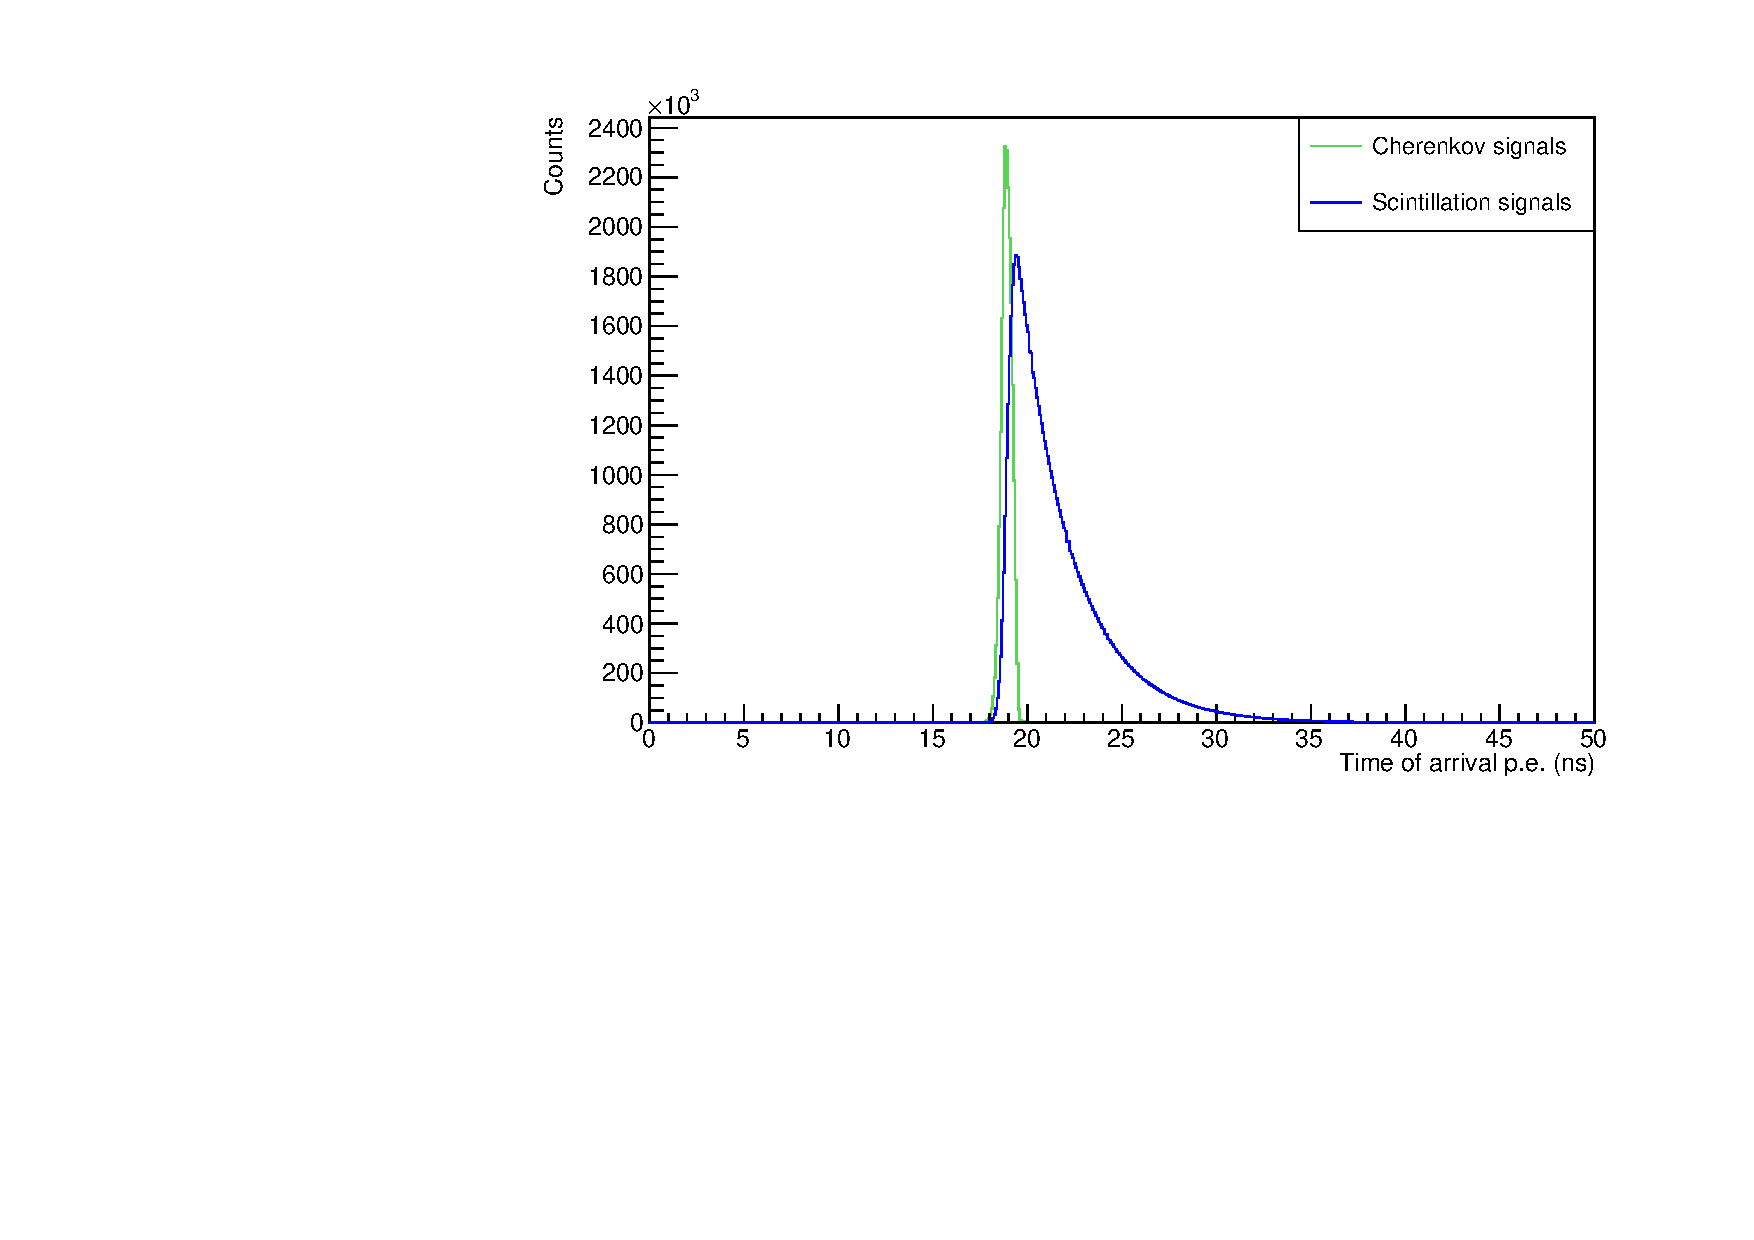
\includegraphics[width=0.8\textwidth]{IMG/Cap5/TrueTimeDist20GeV}
	\caption{The distributions of the time of arrivals of photons on the SiPMs surface, distinguishing the ones transported from Cherenkov fibres from the ones transported from scintillation fibres.}
	\label{fig:true_toa_dist}
\end{figure}

Now a step forward can be done using this data as input for \textit{pySiPM}. The SiPM parameters are chosen as described in paragraph \ref{subsec:SiPM_conf}. In this context the most interesting editable parameter is the decay time constant.\\ 
Figure \ref{fig:top_50ns} and \ref{fig:top_10ns} are in analogy with respect to the last described and presents clearly a widening of the distributions, the cause of this phenomenon has to be associated to the characteristic response function of the sensors \ref{form:resp_func}.\\
These data can be compared looking for differences in changing SiPMs configurations. As we can see in figure \ref{fig:top_per_fib}, the same $C$ and $S$ photons produce narrower time of peak distribution due to the less impact of electronic noise on a sharper response function.\\

\begin{figure}
	\centering
	\subfloat[][\label{fig:top_10ns}$\tau_{fall} = 10\ ns$.]{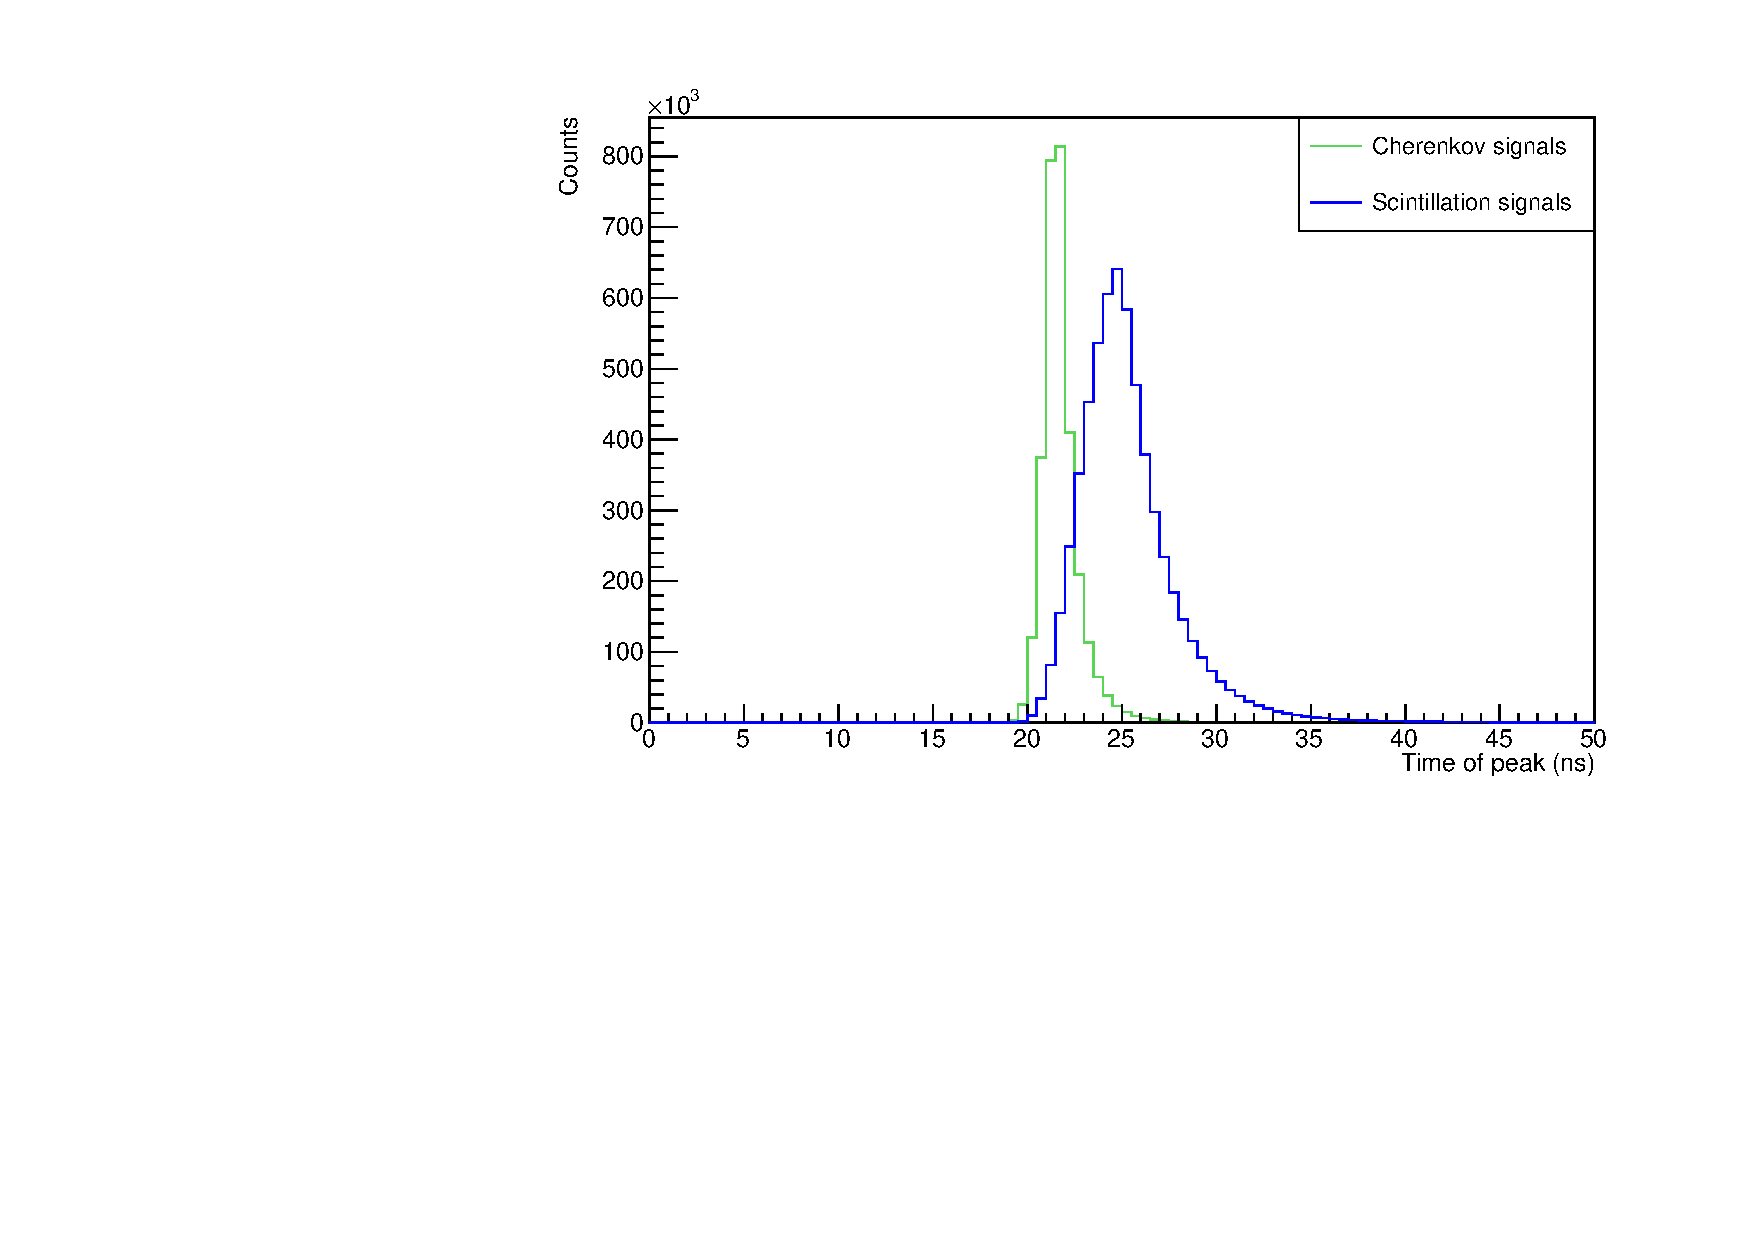
\includegraphics[width=.45\textwidth]{IMG/Cap5/ToP_20GeV_10ns}} \quad
	\subfloat[][\label{fig:top_50ns}$\tau_{fall} = 50\ ns$.]{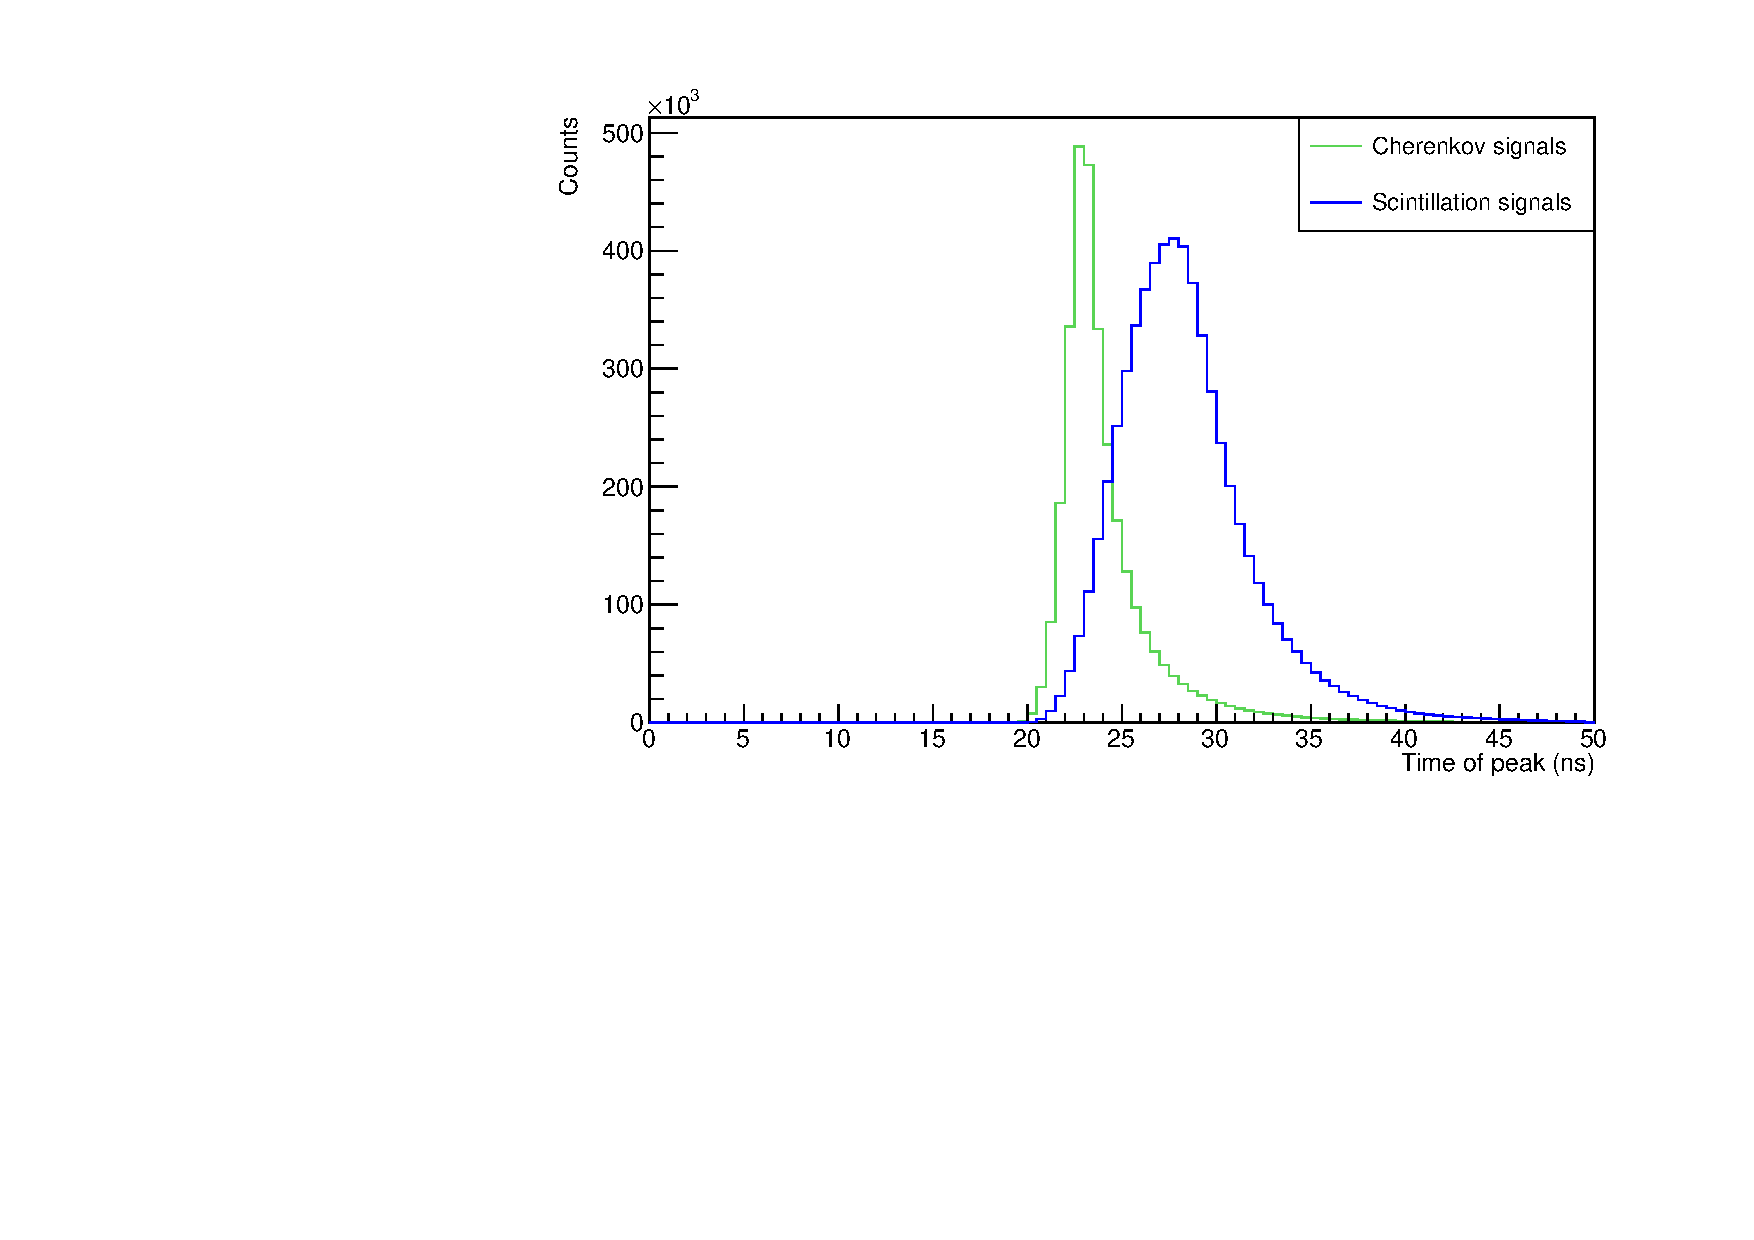
\includegraphics[width=.45\textwidth]{IMG/Cap5/ToP_20GeV_50ns}}
	\caption{Time of peak distributions comparing in each histogram signals from Chernkov and from scintillation fibres. Different figures correspond to different decay time constants.}
	\label{fig:top_per_tau}
\end{figure}

\begin{figure}
	\centering
	\subfloat[][\label{fig:top_C}Cherenkov fibres.]{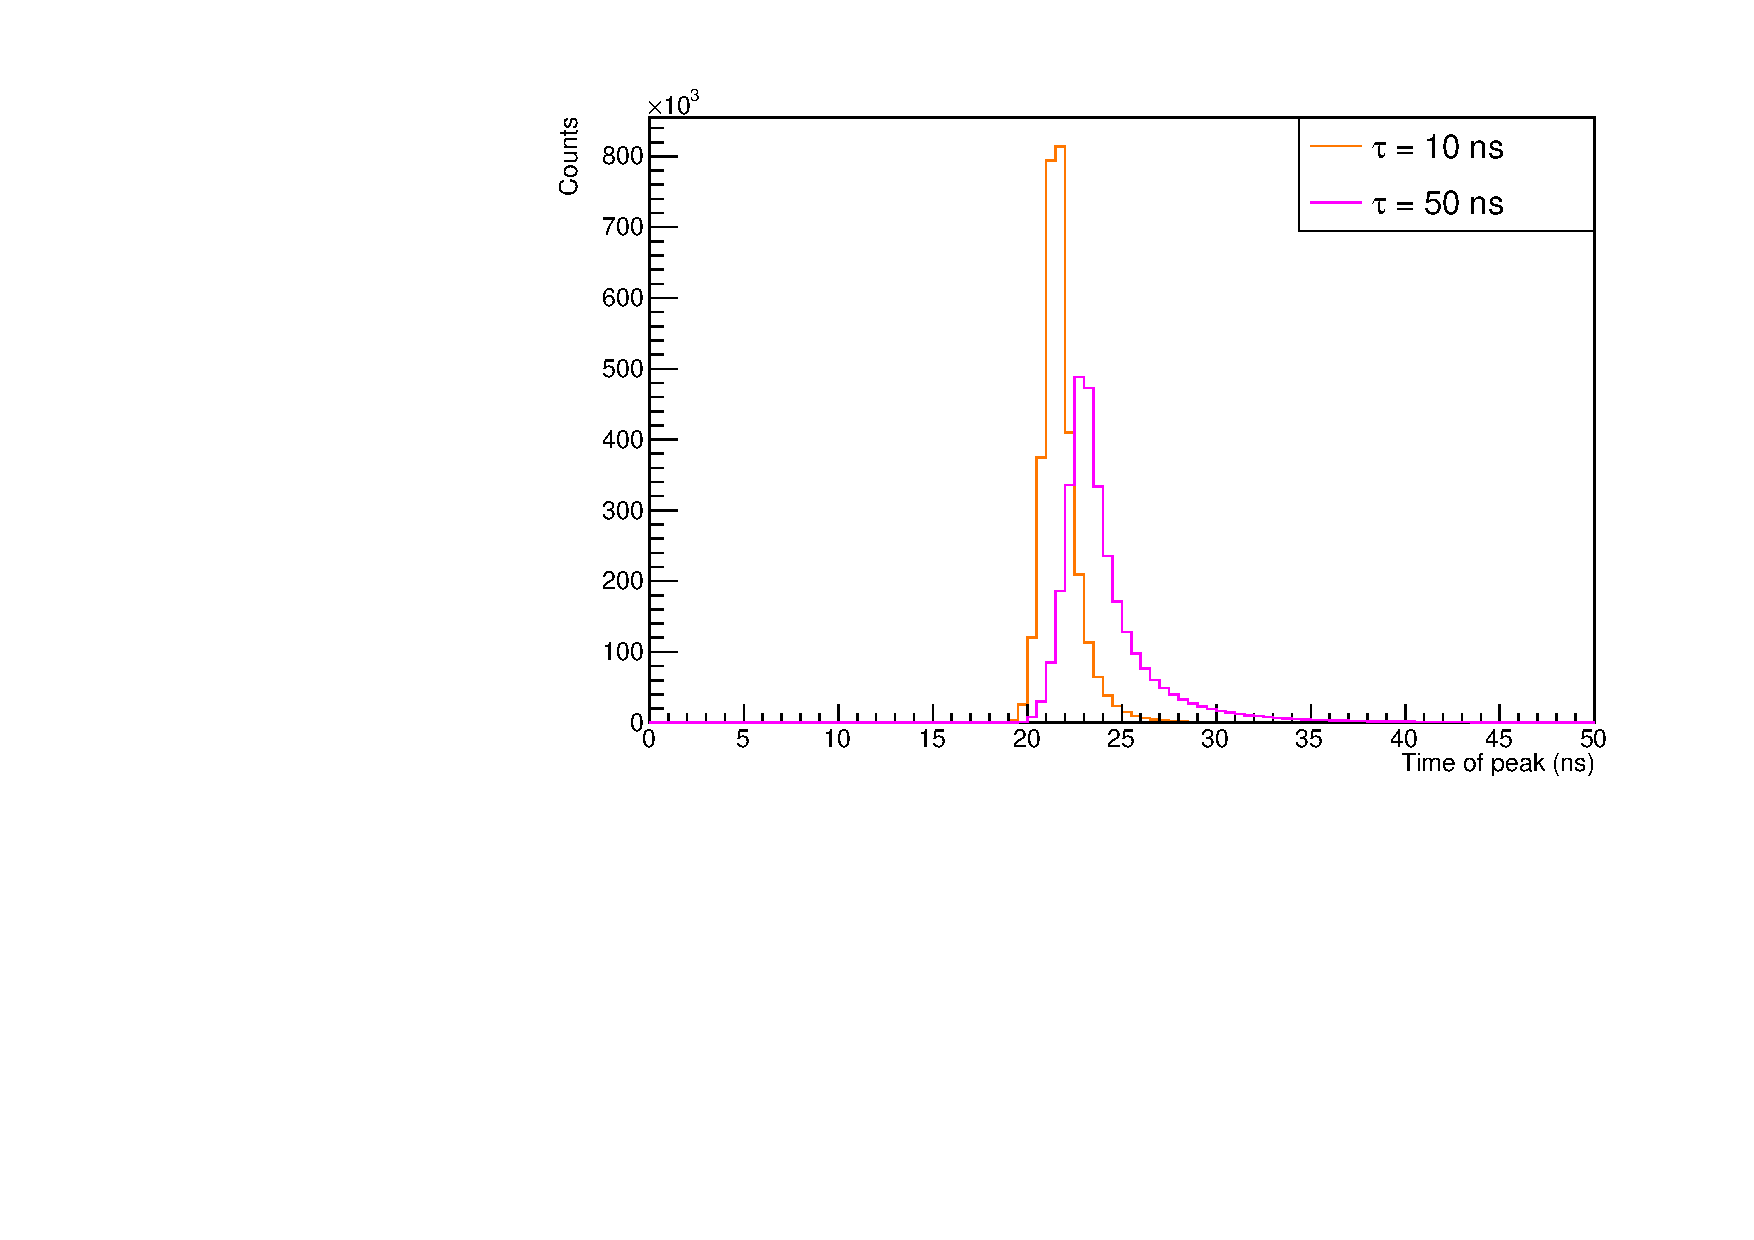
\includegraphics[width=.45\textwidth]{IMG/Cap5/ToP_20GeV_cher}} \quad
	\subfloat[][\label{fig:top_S}Scintillation fibres.]{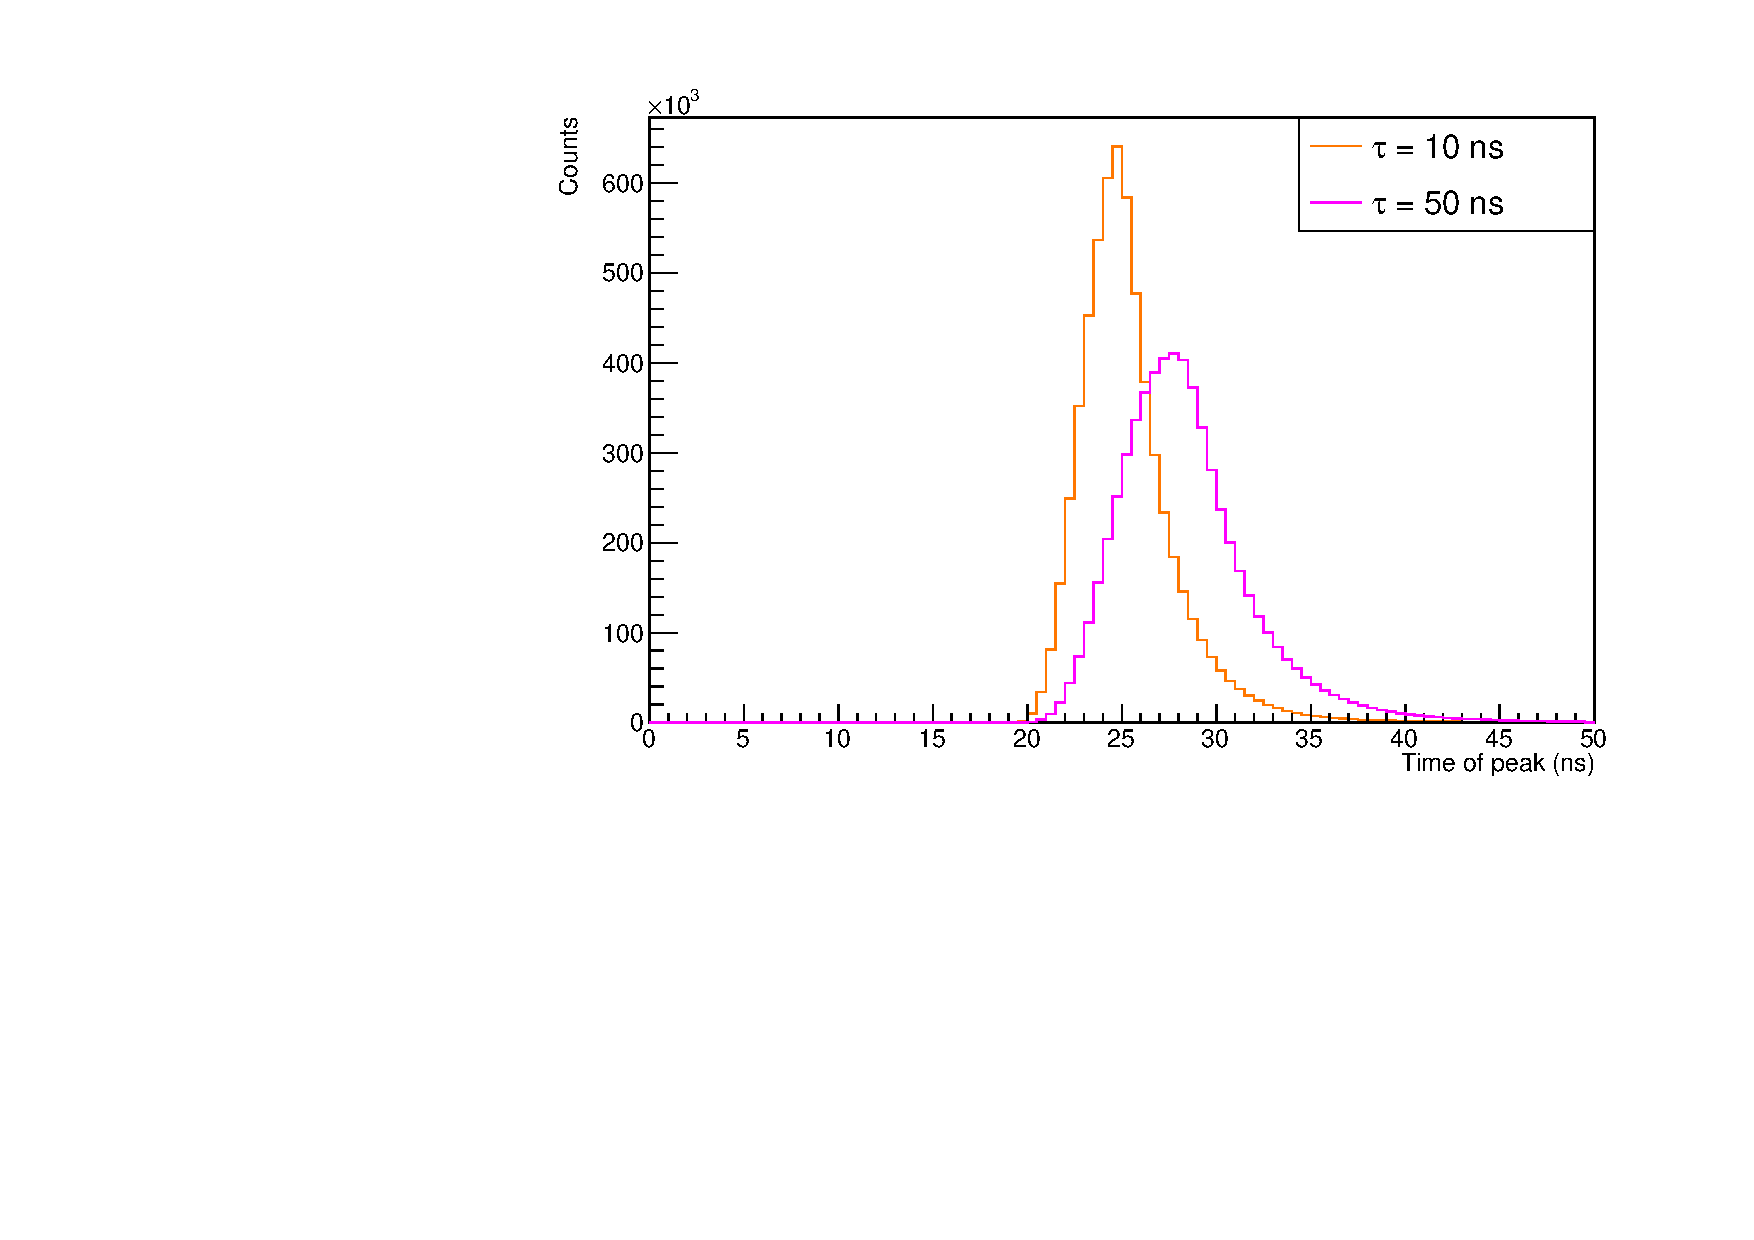
\includegraphics[width=.45\textwidth]{IMG/Cap5/ToP_20GeV_scin}}
	\caption{Time of peak distributions comparing in each histogram signals with different decay time constant of SiPMs. Different figures correspond to different photon emission processes.}
	\label{fig:top_per_fib}
\end{figure}

The impact of noise on time of peak precision is also dependent on the number of photons impinging the same SiPM, in particular the peak precision increase with the number of photons.\\
To prove this $10000$ SiPMs have been fired with an increasing number of simultaneous photons. For each fixed number of photons, the time of peak has been recorded, plotted in an histogram and fitted with a Gaussian function. An example of these histograms is shown in figure \ref{fig:top_dummy}.\\

The standard deviation of these Gaussian fit is the interested quantity that has been recorded and reported in the table \ref{tab:sigmas}.\\
It is interesting to plot these data and study the behavior of the standard deviation in fuction of the number of photons. Figure \ref{fig:top_sigma} shows graphically the data, which are well fitted with a function of the form:
\begin{equation}
	\sigma = \frac{A}{\sqrt{n}} + B.
\end{equation}
The parameters obtained are $A = 0.8712\ ns$ and $B = 0.08734\ ns$ for data associated to SiPMs with $\tau_{fall}=10\ ns$, and $A = 1.949\ ns$ and $B = 0.008217\ ns$ for data associated to SiPMs with $\tau_{fall}=50\ ns$.

\begin{table}
	\centering
	\begin{tabular}{lcc}
		\toprule
		Number of photons	& $\sigma$ with $\tau_{fall}=10\ ns$ (ns) & $\sigma$ with $\tau_{fall}=50\ ns$ (ns)	\\
		\midrule
		$1$ 	& $1.4150$ & $7.0680$ \\
		$2$ 	& $0.8717$ & $2.6420$ \\
		$3$ 	& $0.6738$ & $1.7370$ \\
		$4$ 	& $0.5742$ & $1.3770$ \\
		$5$ 	& $0.5146$ & $1.1230$ \\
		$6$ 	& $0.4624$ & $0.9719$ \\
		$7$ 	& $0.4314$ & $0.9148$ \\
		$8$ 	& $0.3998$ & $0.8508$ \\
		$9$ 	& $0.3811$ & $0.7717$ \\
		$10$ 	& $0.3605$ & $0.7169$ \\
		$25$ 	& $0.2339$ & $0.4481$ \\
		$50$ 	& $0.1679$ & $0.3112$ \\
		$100$ 	& $0.1229$ & $0.2297$ \\
		\bottomrule
	\end{tabular}
	\caption{Standard deviations obtained through the Gaussian fit applied on the time of peak distributions under different conditions. }
	\label{tab:sigmas}
\end{table}

\begin{figure}
	\centering
	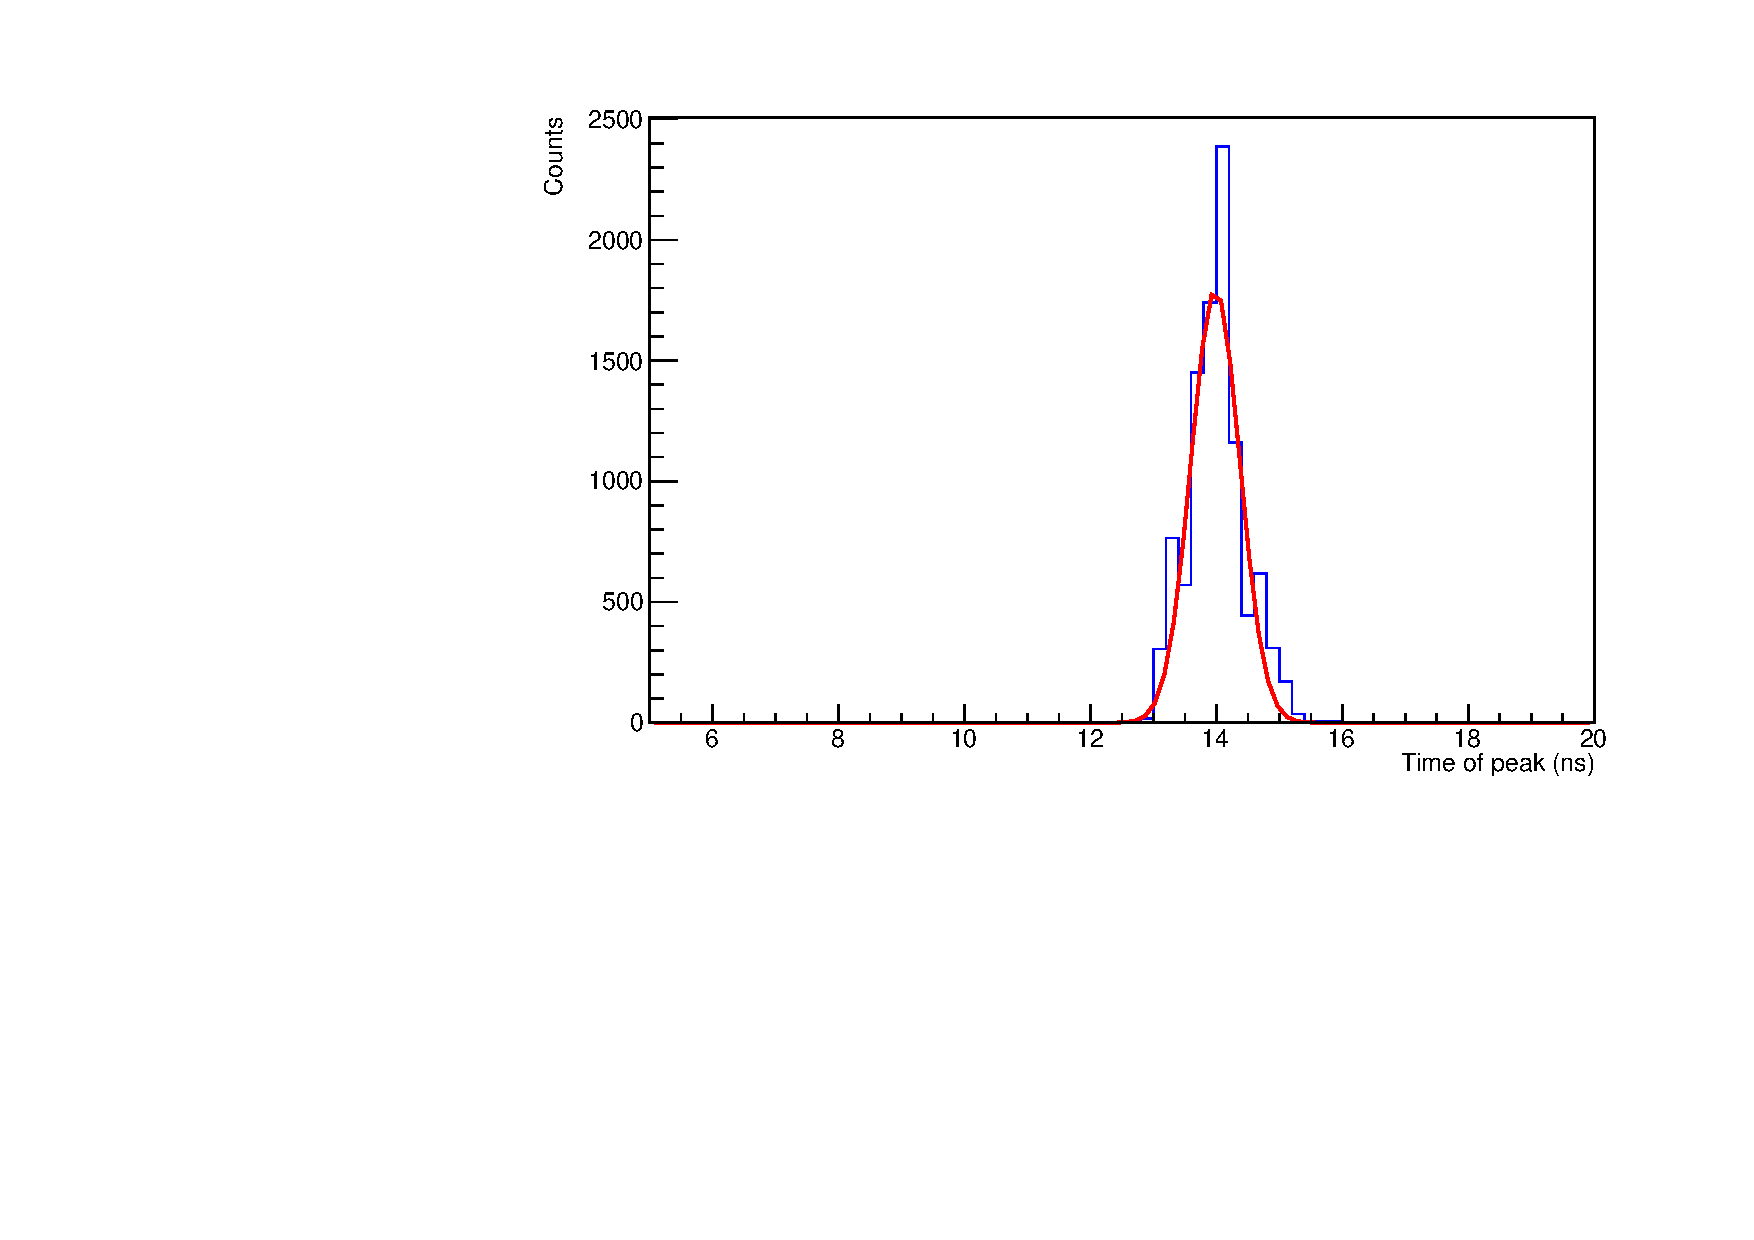
\includegraphics[width=0.8\textwidth]{IMG/Cap5/Dummy11pe_50ns}
	\caption{Time of peak distribution obtained firing $10000$ SiPMs with $11$ photoelectrons each, all at the same time ($10 ns$). Over this distribution a Gaussian fit has been applied.}
	\label{fig:top_dummy}
\end{figure}

\begin{figure}
	\centering
	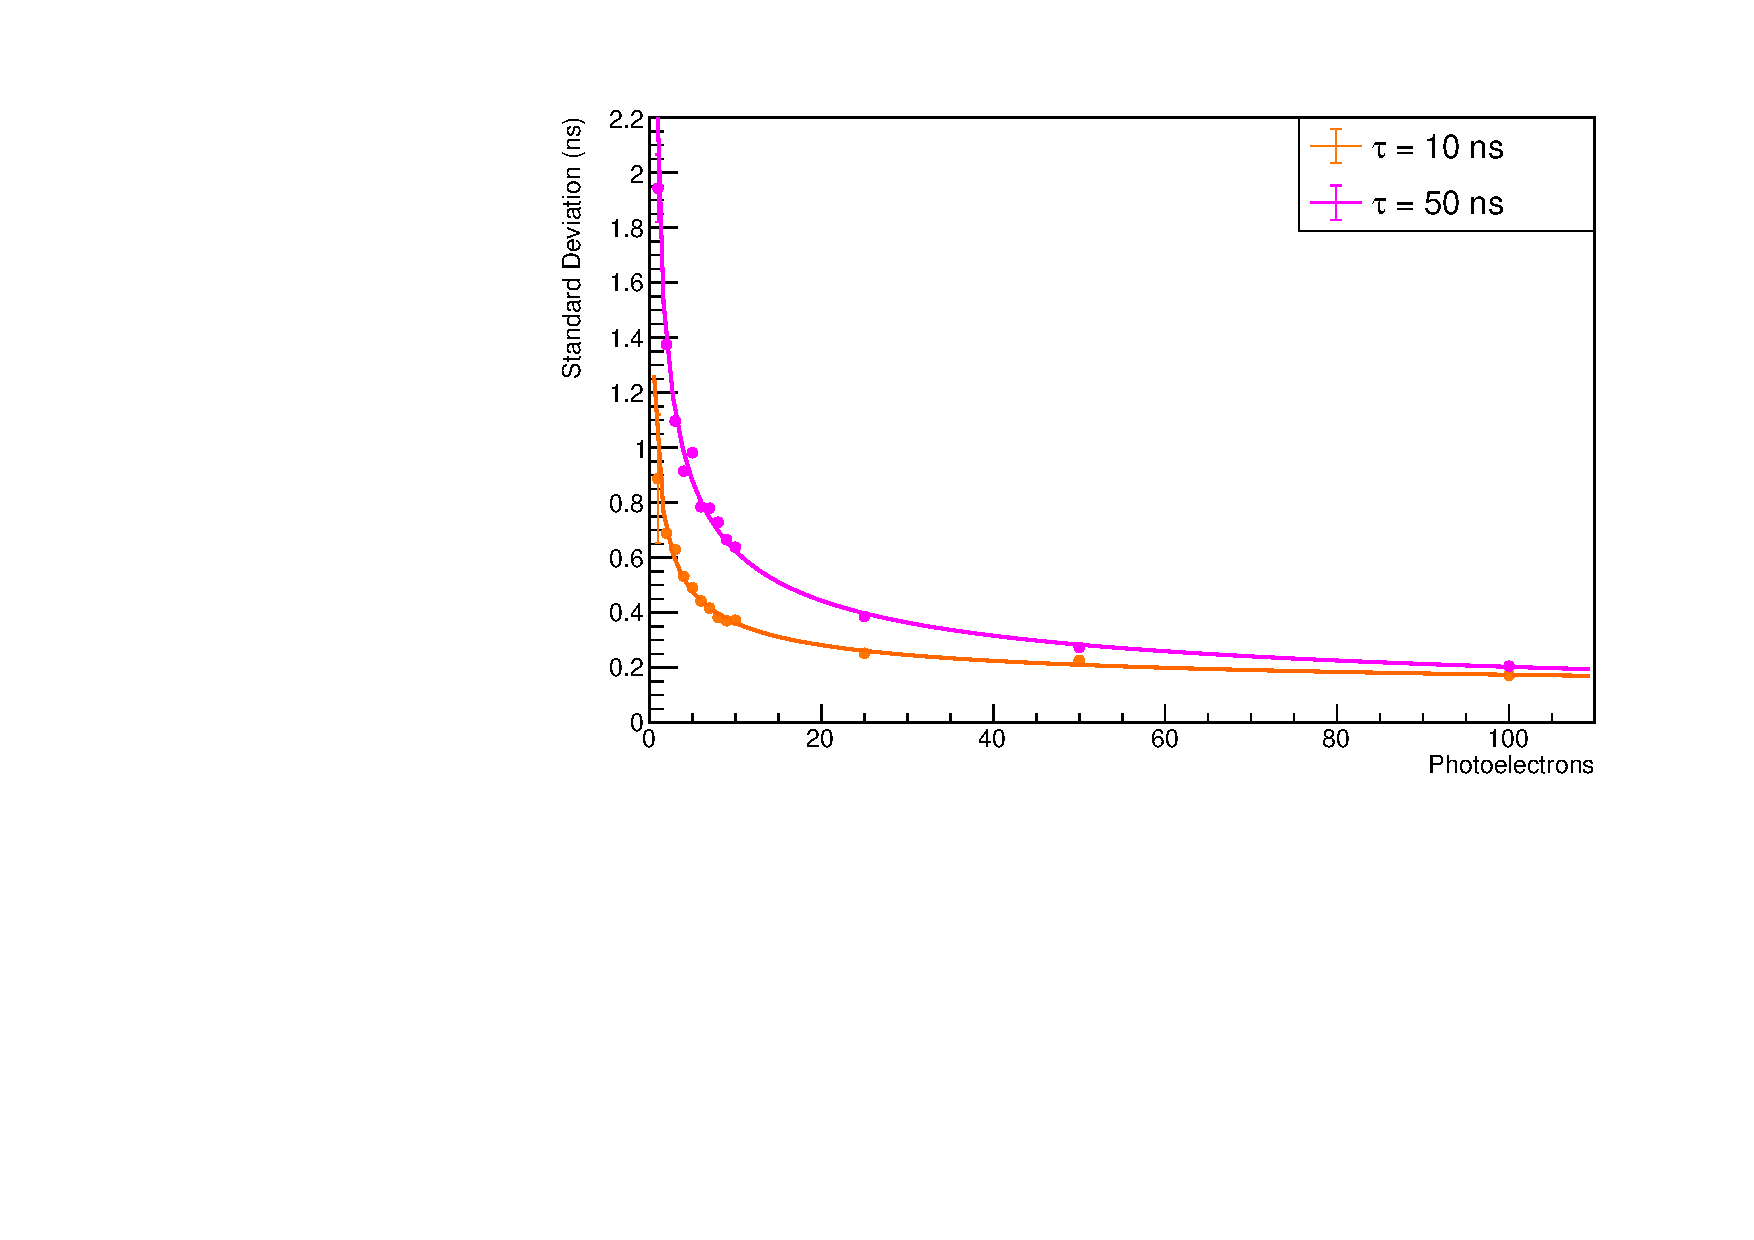
\includegraphics[width=0.8\textwidth]{IMG/Cap5/PeakSpread}
	\caption{Standard deviation behaviour with respect to the number of simultaneous photoelectrons. Study performed with two different decay time constant in SiPMs configuration.}
	\label{fig:top_sigma}
\end{figure}


\subsection{Occupancy effect} \label{subsec:Sat_effect}
The occupancy effect, as shown in the paragraph \ref{subsec:SiPM_work}, is an important characteristic that has to be deeply studied to know the behaviour of the SiPMs under high number of impinging photons and to correctly reconstruct the released energy.\\

As can be seen in figure \ref{fig:sat_example}, this effect is reproduced correctly in our simulations. The example shows the charge integral in dependence to the number of p.e. and follows the concepts already seen in paragraph \ref{subsec:occupancy_teo}.\\

\begin{figure}
	\centering
	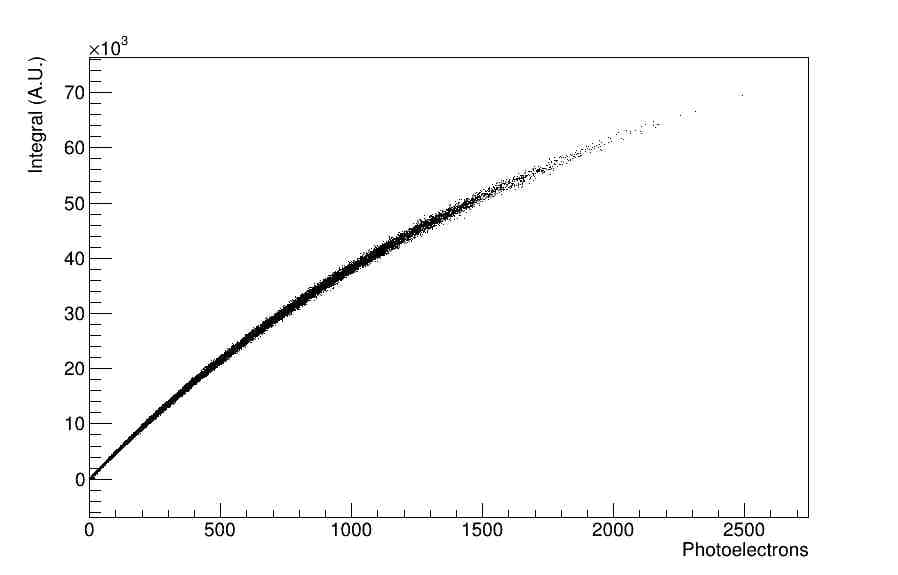
\includegraphics[width=0.7\textwidth]{IMG/Cap5/SatExample.jpg}
	\caption{Example of saturation effect produced with the simulation chain. Each point correspond to a SiPM with a cell size of $25\ \mu m$.}
	\label{fig:sat_example}
\end{figure}

The first step to perform these studies is to reconstruct a calibration law that reproduces the charge integral with respect to the number of p.e. firing the same SiPM.\\
Starting by assuming that in the range of photoelectrons from $2$ to $10$ the saturation effect does not occur in our configurations (i.e. $10000$, $4356$ and $1600$ cells in each SiPM), $10000$ SiPM has been fired $9$ times with an increasing number of simultaneous p.e. in the range considered.\\
To assume that no saturation effect occurs in these data the charge integral distribution from the three different configurations has been compared finding no bias as seen in figure \ref{fig:SatCheck}. The mean and the RMS values has been recorded and fitted with a strait line corresponding to the calibration law desired:
\begin{equation}
	I(n) = A \cdot n + B
\end{equation}
with $A = 49.43 \pm 0.03852$ and $B = 2.491 \pm 0.2516$ (fig \ref{fig:NoSatLine}).\\
The parameter $A$ represents the contribution to the charge integral associated to a single photoelectron. Meanwhile $B$ is the pedestal that is originated mostly by the DCR. This contribution can be evaluated considering our parameters of DCR $= 200\ kH$ and the integration window of $300\ ns$.
$B_{DCR} = 2 \cdot 10^5 \cdot 3 \cdot 10^{-7} p.e. = 6\cdot 10^{-2} p.e. = 6\cdot 10^{-2} \cdot 49.43 = 2.96$.\\
In the following result, the value of the pedestal has been subtracted to the integral value of each SiPM.\\

\begin{figure}
	\centering
	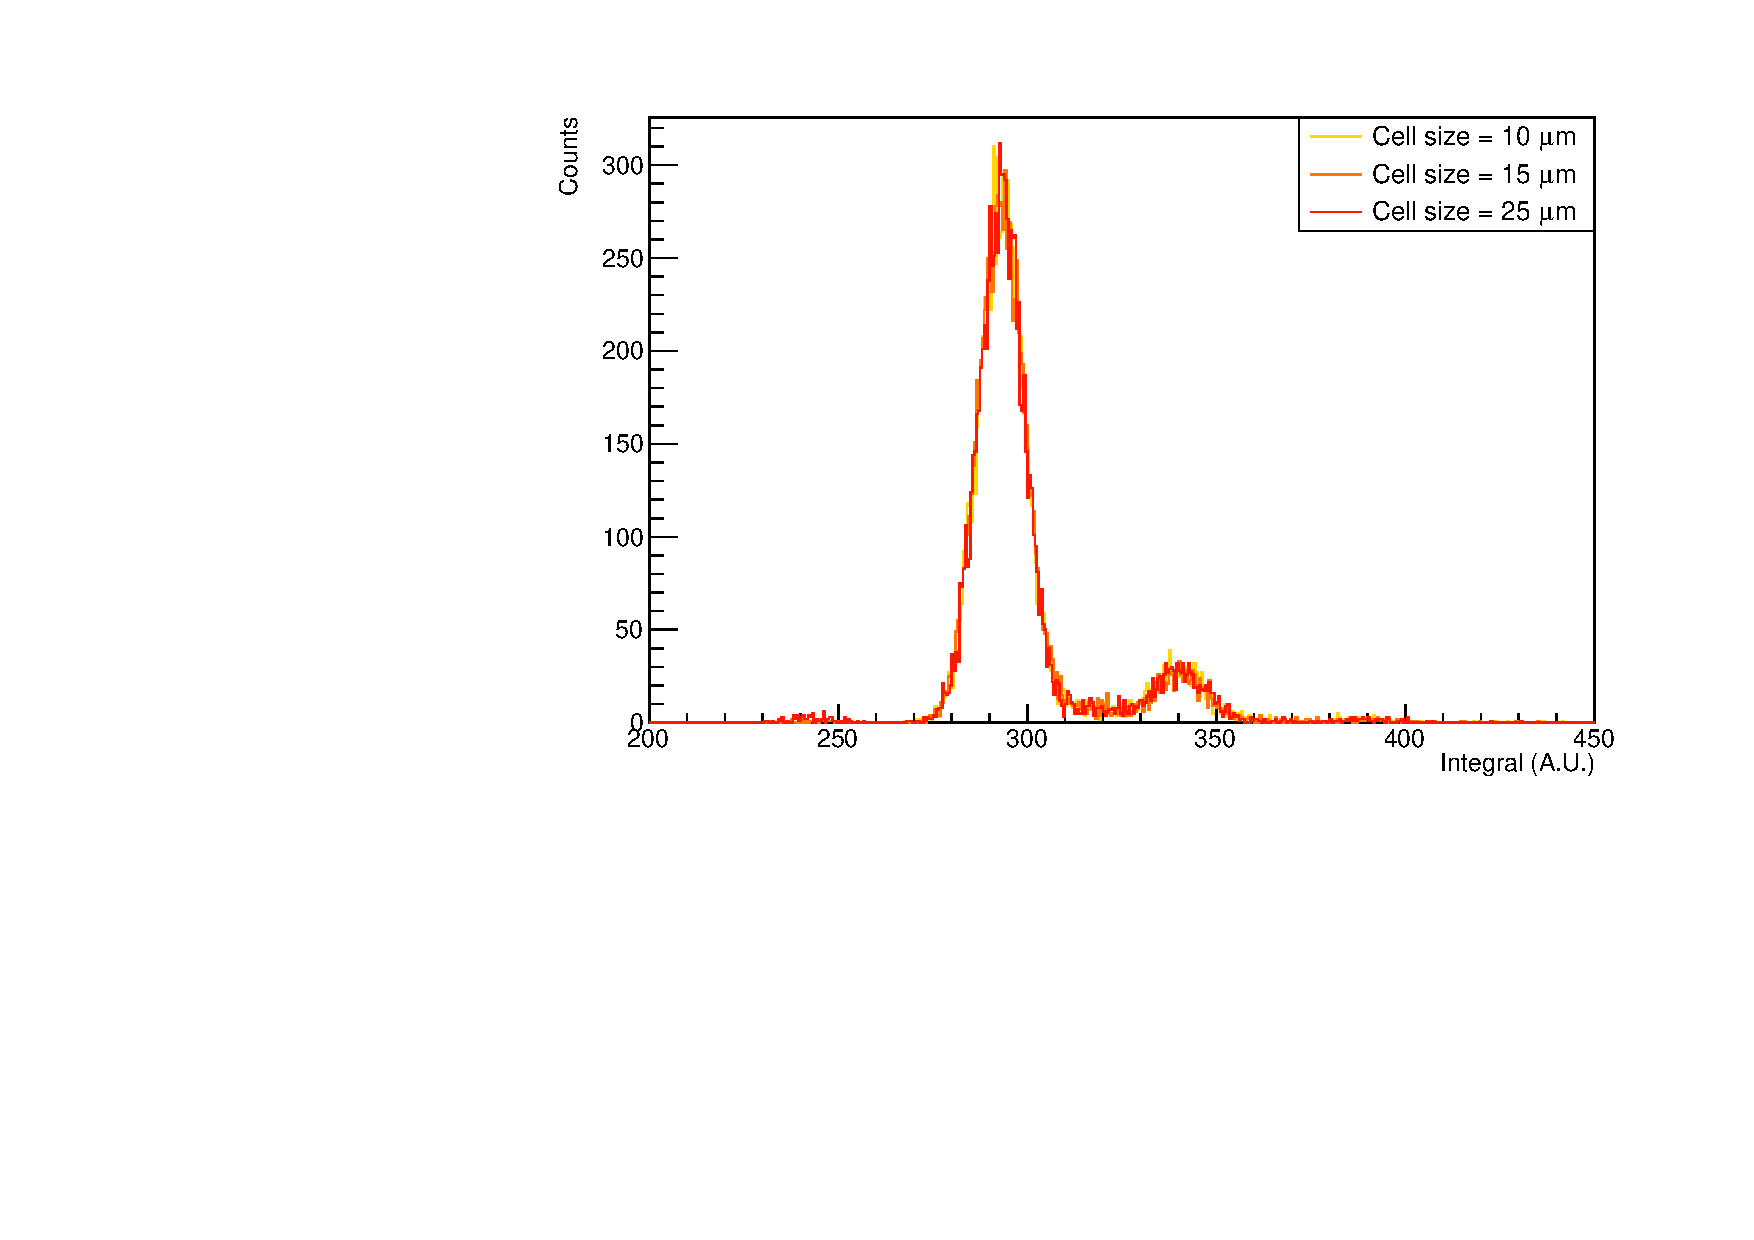
\includegraphics[width=0.7\textwidth]{IMG/Cap5/6pe_sat}
	\caption{Charge integral distributions with different SiPM cell size considering $6$ simultaneous photoelectrons. The distribution shape with less then $10$ simultaneous p.e. is not dependent to the number of cells.}
	\label{fig:SatCheck}
\end{figure}

\begin{figure}
	\centering
	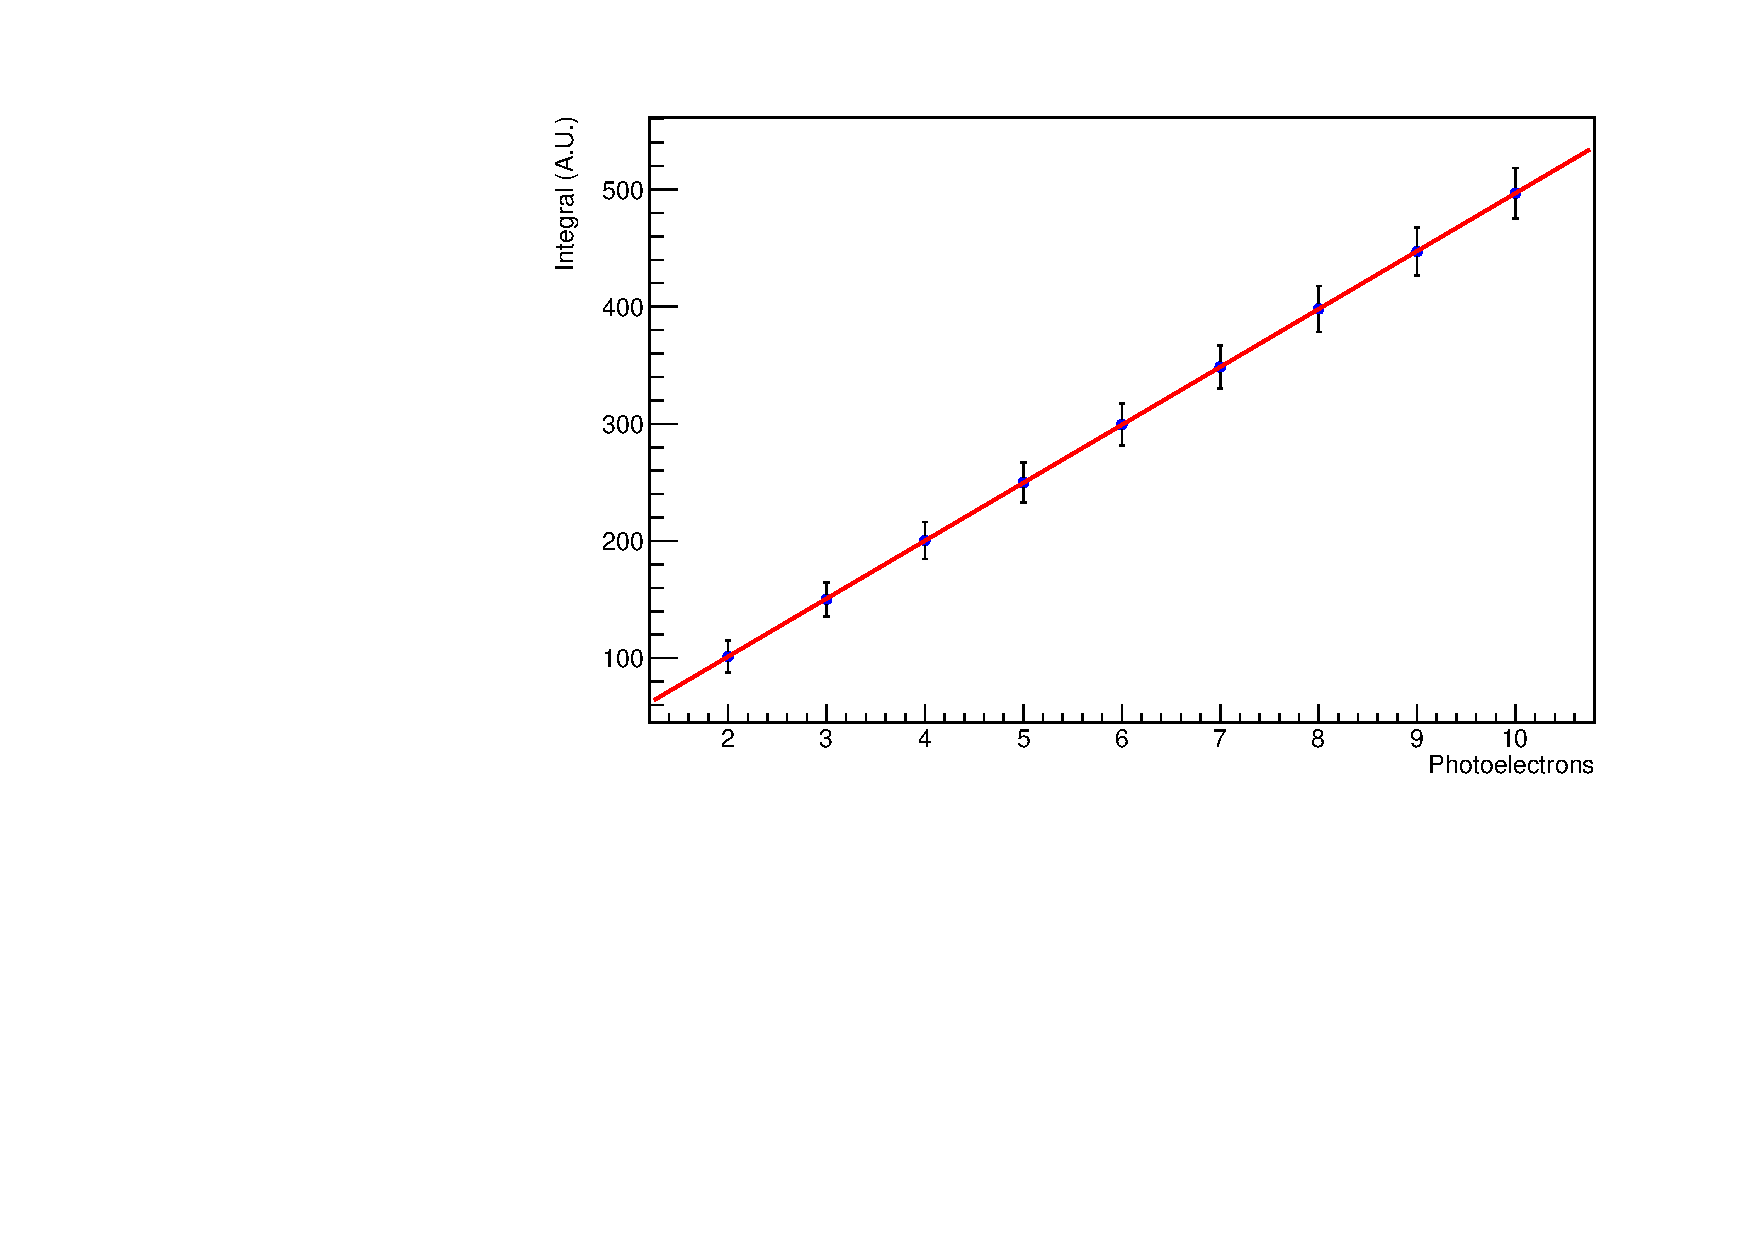
\includegraphics[width=0.7\textwidth]{IMG/Cap5/NoSatLine}
	\caption{Study of the proportional relation between integral and number of photoelectrons in the range from $2$ to $10$. A linear fit has been applied to find calibration law without saturation.}
	\label{fig:NoSatLine}
\end{figure}

The occupancy effect has been studied in electromagnetic shower produced by single electrons of different energies at each event with discrete values of $20,\ 40,\ 60,\ 80\ GeV$.\\
The impact of the saturation has been quantified using the line $I = A\cdot n$ as no saturation reference. The result obtained from $10000$ events of single $40\ GeV\ e^-$ with different SiPM configurations are separated in Cherenkov and Scintillation signals. They are shown in figure \ref{fig:sat_fibres} where each point correspond to a single SiPM. The smaller is the number of cells, the greater is the occupancy effect.\\
Moreover, as expected, the scintillation fibres transport $\sim 4$ times the p.e. from Cherenkov ones on average, therefore they are more affected to the saturation.\\

\begin{figure}
	\centering
	\subfloat[][Cherenkov signals.]{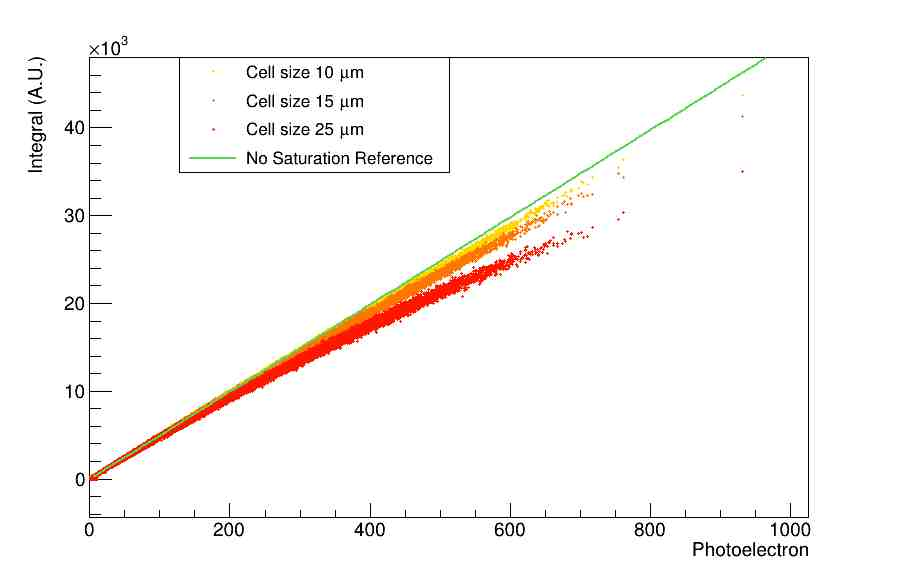
\includegraphics[width=.7\textwidth]{IMG/Sat_Fib_40GeV_cher}} \\
	\subfloat[][Scintillation signals.]{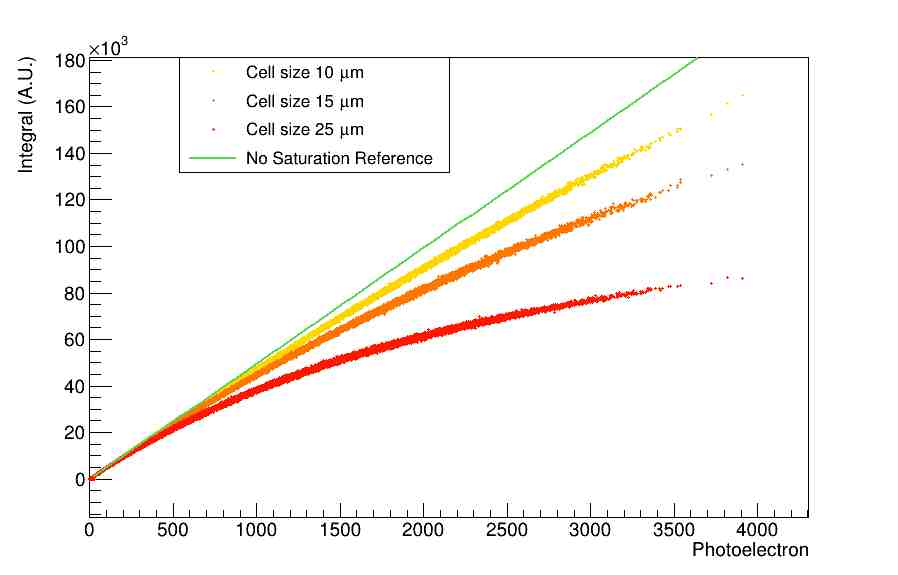
\includegraphics[width=.7\textwidth]{IMG/Sat_Fib_40GeV_scin}}
	\caption{The plots, divided considering the two different photon production processes, show the occurrence of the occupancy effect studying single $40\ GeV$ electrons. Each point correspond to a SiPM with different values of cell size. The no saturation line shown in figure \ref{fig:NoSatLine} has been added as reference.}
	\label{fig:sat_fibres}
\end{figure}

This process can be extended considering one event at the time and adding the charge integral and the corresponding number of photoelectrons. The effect produced is represented in figure \ref{fig:sat_events} where each point correspond to a single event.\\

\begin{figure}
	\centering
	\subfloat[][Cherenkov signals.]{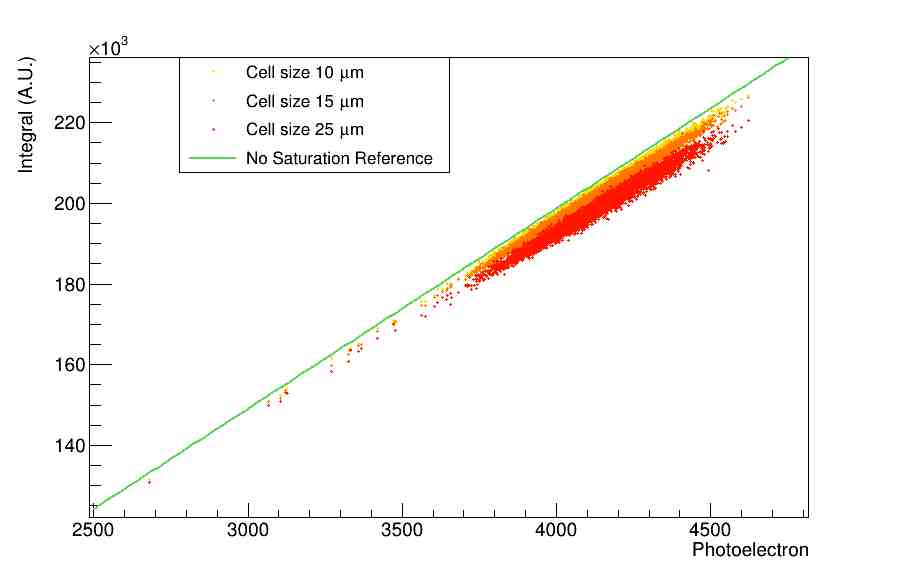
\includegraphics[width=.7\textwidth]{IMG/Sat_Ev_40GeV_cher}}\\
	\subfloat[][Scintillation signals.]{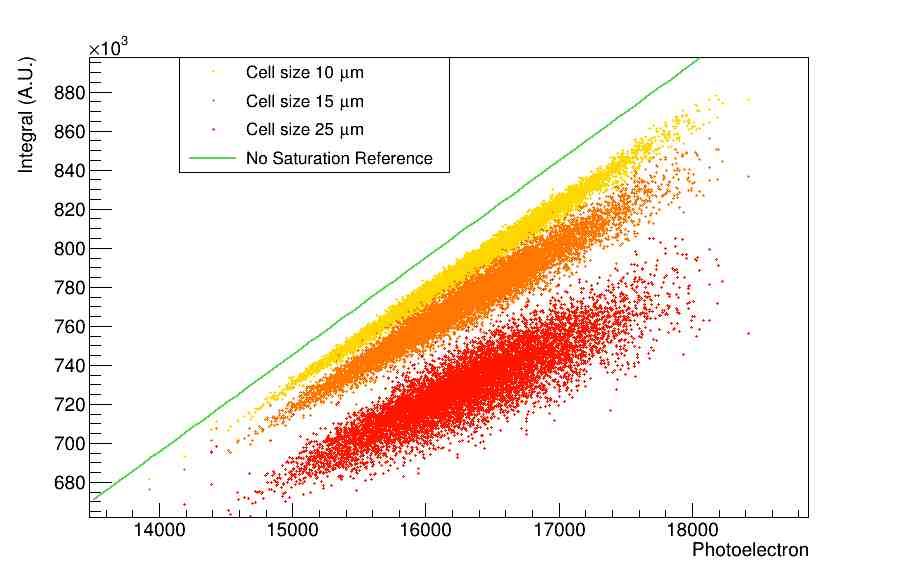
\includegraphics[width=.7\textwidth]{IMG/Sat_Ev_40GeV_scin}}
	\caption{The plots, divided considering the two different photon production processes, show the occurrence of the occupancy effect studying single $40\ GeV$ electrons. Each of the $10000$ points correspond to a single event where integral and number of photoelectrons have been added over the fired SiPMs. Different values of cell size are represented with different colors. The no saturation line shown in figure \ref{fig:NoSatLine} has been added as reference.}
	\label{fig:perc_sat}
\end{figure}

As can be seen, the occupancy effect in our conditions is consistent. To mitigate this problem an analytical correction can be performed through the formula:
\begin{equation}
	N_{fired}=N_{cells} \cdot \left[ 1 - \exp\left(-\frac{N_{p.e.}}{N_{cells}}\right)\right]
\end{equation}

therefore the correction has been applied modifying the integral values such as:
\begin{equation}
	I_{corr} = - A N_{cells} \left[ \ln\left(1 - \frac{I}{A N_{cells}}\right) \right]
\end{equation}

The results obtained can be visualized in figure \ref{fig:sat_corr} where are compared the data from SiPM with cell size of $10\ \mu m$ with and without analytical correction.


\begin{figure}
	\centering
	\subfloat[][Cherenkov signals. Points are single SiPMs.]{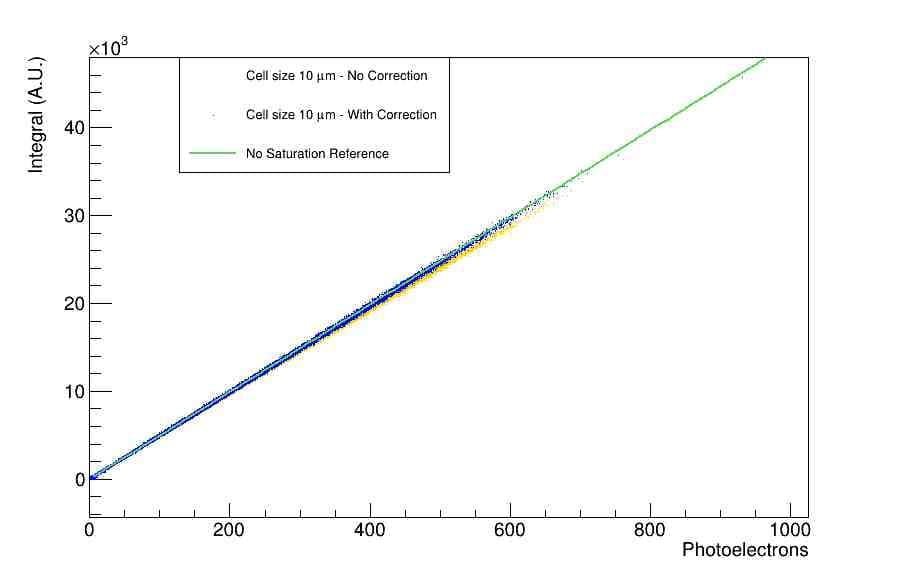
\includegraphics[width=.5\textwidth]{IMG/Cap5/SatCorr_40GeV_fib_cher}}\quad
	\subfloat[][Scintillation signals. Points are single SiPMs.]{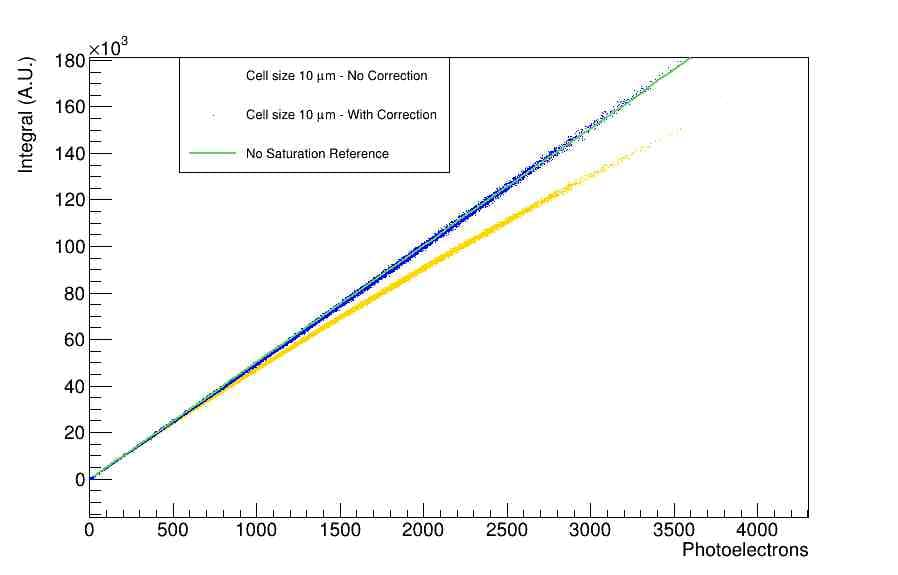
\includegraphics[width=.5\textwidth]{IMG/Cap5/SatCorr_40GeV_fib_scin}}\\
	\subfloat[][Cherenkov signals. Points are single events.]{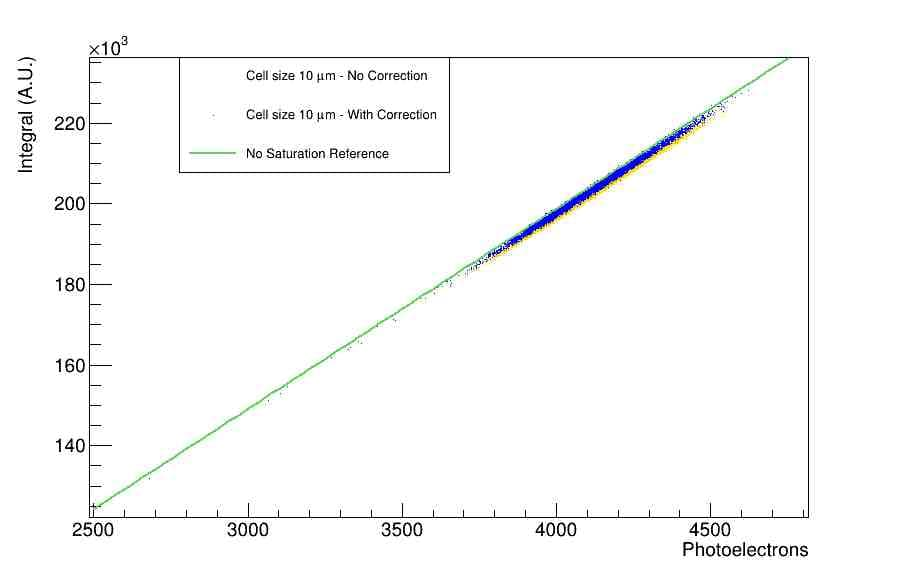
\includegraphics[width=.5\textwidth]{IMG/Cap5/SatCorr_40GeV_ev_cher}} \quad
	\subfloat[][Scintillation signals. Points are single events.]{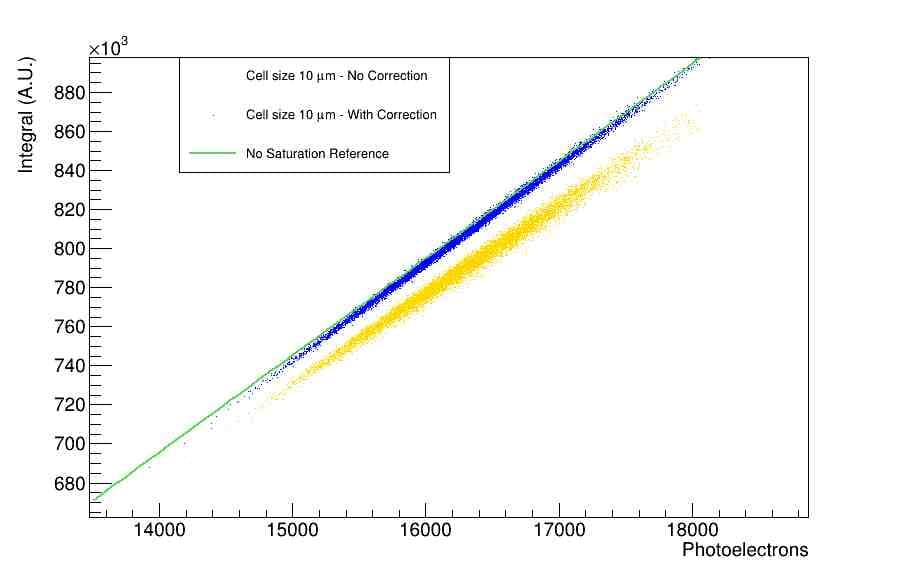
\includegraphics[width=.5\textwidth]{IMG/Cap5/SatCorr_40GeV_ev_scin}}
	\caption{Similar plots to figures \ref{fig:sat_fibres} and \ref{fig:sat_events}. Two series of data are presented to show the effectiveness of the analytical correction. The no saturation line shown in figure \ref{fig:NoSatLine} has been added as reference. }
	\label{fig:sat_corr}
\end{figure}

The discrepancy from the no saturation reference quantifies the effect of the occupancy when performing the energy reconstruction task. The percentage difference has been evaluated through the formula $\frac{E_{NoSat}-E}{E_{NoSat}}$, and the value obtained fill the histograms in figure \ref{fig:perc_sat}.\\
After applying the analytical correction a clear improvement is show in figures \ref{fig:sat_corr_perc}.\\

\begin{figure}
	\centering
	\subfloat[][Cherenkov signals.]{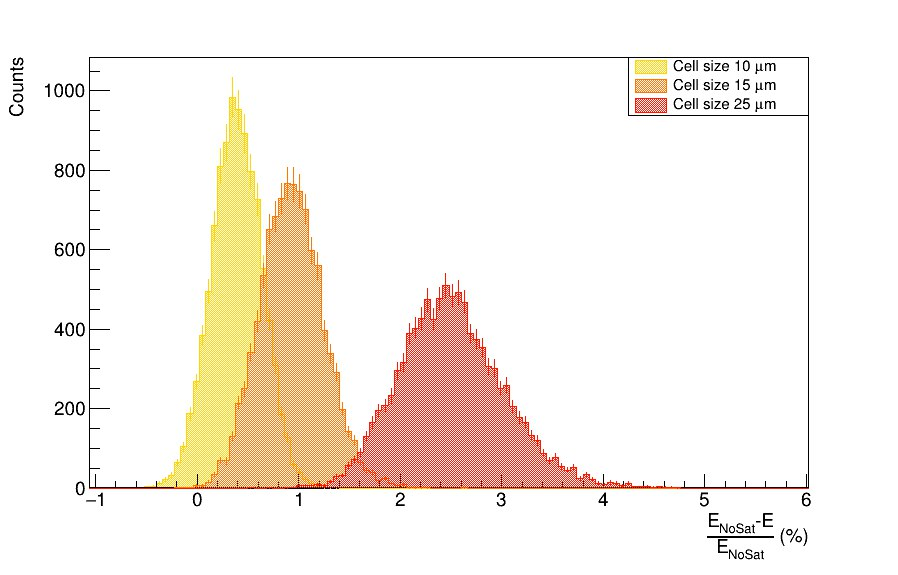
\includegraphics[width=.5\textwidth]{IMG/PercEnergy_40GeV_cher.jpg}} \quad
	\subfloat[][Scintillation signals.]{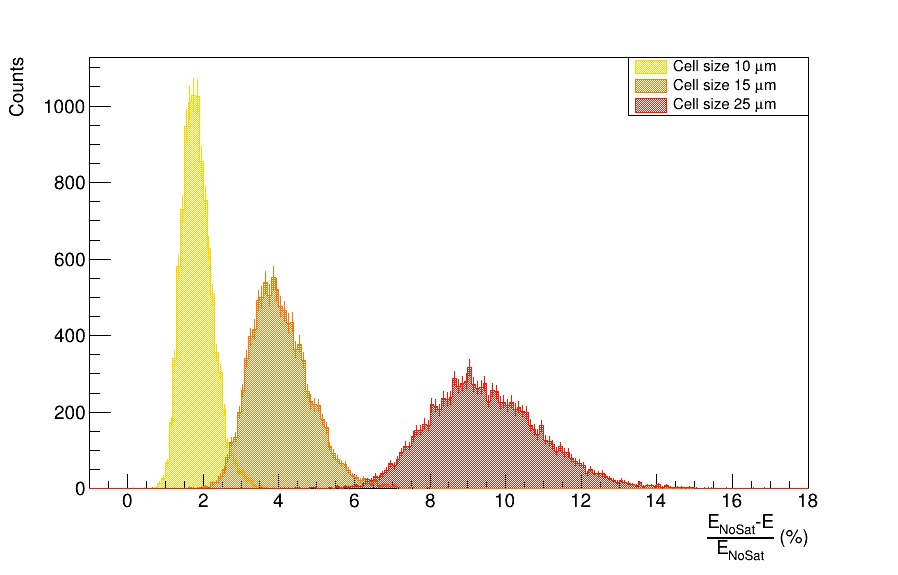
\includegraphics[width=.5\textwidth]{IMG/PercEnergy_40GeV_scin.jpg}}
	\caption{Percentage discrepancy distribution considering events with single 40GeV electrons. Different colors correspond to different cell size values.}
	\label{fig:sat_events}
\end{figure}

\begin{figure}
	\centering
	\subfloat[][Cherenkov signals.]{\includegraphics[width=.5\textwidth]{IMG/Cap5/PercEnergy_40GeV_corr_cher}} \quad
	\subfloat[][Scintillation signals.]{\includegraphics[width=.5\textwidth]{IMG/Cap5/PercEnergy_40GeV_corr_scin}}
	\caption{Percentage discrepancy distribution considering events with single 40GeV electrons to evaluate the effect of the analytical correction applied on data obtained with a cell size of $10\ \mu m$.}
		\label{fig:sat_corr_perc}
\end{figure}

This whole process has been performed simulating electrons with energies of $20,\ 40,\ 60,\ 80\ GeV$. Mean and standard deviation of the gaussian fit applied on the percentage discrepancy have been recorded and the obtained plots are shown in figure \ref{fig:sat_vs_E}.\\

\begin{figure}
	\centering
	\subfloat[][Cherenkov signals.]{\includegraphics[width=.7\textwidth]{IMG/Cap5/PercEnergy_cher}} \\
	\subfloat[][Scintillation signals.]{\includegraphics[width=.7\textwidth]{IMG/Cap5/PercEnergy_scin}}
	\caption{Percentage discrepancy behaviour with respect to the primary particle energy. Different cell sizes are compared also with data obtained performing the analytical correction.}
	\label{fig:sat_vs_E}
\end{figure}

\subsection{Energy resolution} \label{subsec:E_res}
The first step to study the energy resolution is to calibrate the full simulation.\\
Dual-readout calorimeters are typically calibrated at the electromagnetic scale. This is specially useful in a leptonic collider because, having easily access to electrons and positrons, the calorimeter can be calibrated precisely during all the life of the experiment.\\

The calibration has been performed on $40\ GeV$ electrons applying the one-suppression already introduce in paragraph \ref{subsec:Sim_SiPM}. $10000$ events with single $40\ GeV$ electrons have been fired from the interaction point obtaining the charge integral distributions for scintillation and Cherenkov signals.% shown in figure \ref{fig:int_dist}.
The calibration constants obtained to transform these data in energy distributions centered around $40\ GeV$ are: $k_S = 4.998 \times 10^{-5}$ and $k_C = 2.023 \times 10^{-4}$.\\
Two analogue calibration constants have been obtained starting from the number of photoelectrons distribution with values of:  $k_{pe,S} = 2.48 \times 10^{-3}$ and $k_{pe,C} = 1.00 \times 10^{-2}$.\\

%\begin{figure}
%	\centering
%	\subfloat[][Cherenkov signals.]{\includegraphics[width=.7\textwidth]{IMG/Intdist_40GeV_cher_cal}} \\
%	\subfloat[][Scintillation signals.]{\includegraphics[width=.7\textwidth]{IMG/Intdist_40GeV_scin_cal}}
%	\caption{Integral distrib.}
%	\label{fig:int_dist}
%\end{figure}

Starting from these calibration constant, the energy distributions can be obtained from the number of p.e. (pre SiPM digitization simulation) of from the charge integral (post SiPM digitization simulation). The two types of distribution are compared in figure \ref{fig:cfr_e_dist}.\\
As expected, the energy distributions obtained from the charge integrals are wider due to the introduction of the electronic noise. However, the effect is minimal considering the fact that in each event hundreds of SiPMs are active and the white noise has mean zero.\\

\begin{figure}
	\centering
	\subfloat[][Cherenkov signals.]{\includegraphics[width=.7\textwidth]{IMG/Cap5/E_hist_cfr_cher}} \\
	\subfloat[][Scintillation signals.]{\includegraphics[width=.7\textwidth]{IMG/Cap5/E_hist_cfr_scin}}
	\caption{Charge integral distributions generated with data from GEANT4 (\textit{pre pySiPM}) or from the full simulation (\textit{post pySiPM}). The histograms are shifted by their mean values to show the minimal difference in the distributions spread.}
	\label{fig:cfr_e_dist}
\end{figure}

The energy distributions have been fitted with a Gaussian function to obtain mean, standard deviation e respective errors. Doing this with different primary electron energies the energy resolution can be studied. Mean and standard deviation are listed in tables \ref{tab:e_res_int} \ref{tab:e_res_pe}.\\
Then fitting the $\sigma/E$ values in the energy range $20-80\ GeV$ can be seen there is a good agreement with the functions:
\begin{equation}\label{eq:resolution}
	\frac{\sigma}{E} = \frac{A_1}{\sqrt{E}} + B_1 \qquad \text{or} \qquad \frac{\sigma}{E} = \frac{A_2}{\sqrt{E}} \oplus B_2
\end{equation} 
as shown in figure \ref{fig:sigma_su_e}, with the fit parameters listed in table \ref{tab:res_regular_sum} and \ref{tab:res_quadratic_sum}. The plots also show the loss of resolution with the introduction of the SiPM digitization software.\\

\begin{table}
	\centering
	\begin{tabular}{lccc}
		\toprule
		& True E (GeV) & Mean E (GeV) & Standard Deviation (GeV) \\
		\midrule
		\textbf{Scintillation} &	$20$ 	& $19.90$ & $0.95$ \\
		& $40$ 	& $40.00$ & $1.44$ \\
		& $60$ 	& $60.65$ & $1.85$ \\
		& $80$ 	& $81.18$ & $2.26$ \\
		\midrule
		\textbf{Cherenkov} & $20$ 	& $19.88$ & $0.95$ \\
		& $40$ 	& $40.00$ & $1.42$ \\
		& $60$ 	& $60.61$ & $1.73$ \\
		& $80$ 	& $81.12$ & $2.08$ \\
		\bottomrule
	\end{tabular}
	\caption{Mean and standard deviation obtained by fitting with Gaussian function the energy distributions. The data are obtained with results from the full simulation.}
	\label{tab:e_res_int}
\end{table}

\begin{table}
	\centering
	\begin{tabular}{lccc}
		\toprule
		& True E (GeV) & Mean E (GeV) & Standard Deviation (GeV) \\
		\midrule
		\textbf{Scintillation} &	$20$ 	& $19.82$ & $0.92$ \\
		& $40$ 	& $40.00$ & $1.39$ \\
		& $60$ 	& $60.28$ & $1.78$ \\
		& $80$ 	& $81.58$ & $2.16$ \\
		\midrule
		\textbf{Cherenkov} & $20$ 	& $19.76$ & $0.92$ \\
		& $40$ 	& $40.00$ & $1.36$ \\
		& $60$ 	& $60.40$ & $1.66$ \\
		& $80$ 	& $81.86$ & $1.91$ \\
		\bottomrule
	\end{tabular}
	\caption{Mean and standard deviation obtained by fitting with Gaussian function the energy distributions. The data are obtained with results from DR calorimeter simulation applying the calibration from the photoelectrons number.}
	\label{tab:e_res_pe}
\end{table}

\begin{figure}
	\centering
	\subfloat[][$C$ signals.]{\includegraphics[width=.8\textwidth]{IMG/Res_cher}} \\
	\subfloat[][$S$ signals.]{\includegraphics[width=.8\textwidth]{IMG/Res_scin}}
	\caption{Calorimeter resolution plot where the data have been fitted with the formula on the left of line \ref{eq:resolution}.}
	\label{fig:sigma_su_e}
\end{figure}

\begin{table}
	\centering
	\begin{tabular}{lcc}
		\toprule
		& \textbf{Scintillation} & \textbf{Cherenkov} \\
		\midrule
		\textbf{pre pySiPM} &	$\frac{17.39\%}{\sqrt{E}}+0.37\%$ 	& $\frac{21.13\%}{\sqrt{E}}+0.01\%$ \\
		\textbf{post pySiPM} & $\frac{17.84\%}{\sqrt{E}}+0.77\%$ 	& $\frac{20.01\%}{\sqrt{E}}+0.30\%$ \\
		\bottomrule
	\end{tabular}
	\caption{Fit results on the energy resolution using the functional form \ref{eq:resolution} on the left.}
	\label{tab:res_regular_sum}
\end{table}

\begin{table}
	\centering
	\begin{tabular}{lcc}
		\toprule
		& \textbf{Scintillation} & \textbf{Cherenkov} \\
		\midrule
		\textbf{pre pySiPM} &	$\frac{19.78\%}{\sqrt{E}}\oplus1.55\%$ 	& $\frac{21.21\%}{\sqrt{E}}\oplus0.07\%$ \\
		\textbf{post pySiPM} & $\frac{20.14\%}{\sqrt{E}}\oplus1.62\%$ 	& $\frac{21.04\%}{\sqrt{E}}\oplus0.98\%$ \\
		\bottomrule
	\end{tabular}
	\caption{Fit results on the energy resolution using the functional form \ref{eq:resolution} on the right.}
	\label{tab:res_quadratic_sum}
\end{table}

		%--------CAPITOLO 5--------
		\chapter{Neural Network: Particle ID on imaging} \label{sec:NN_img}
Neural network and machine learning algorithm are powerful and versatile instruments that can improve the process of data analysis learning from datasets and making prediction with a certain degree of accuracy. Modern science, including physics, is taking more and more advantage of these techniques as the years go by.
The availability of big data is a key aspect in performing these studies and experimental particle physics is an area that can provide large datasets.\\

The chapter describes a possible application of deep neural networks on data generated through the IDEA DR Calorimeter full simulation with the aim to obtain simple particle identification analyzing the spatial deposited energy distribution.\\
An introduction to the computational techniques is provided, briefly describing the role of each component and the common structures that are used to perform the study.\\

All the data have to be prepared to be used in a neural network structure, the section \ref{sec:NN_data} shows which information has been used and how it has been processed to be analyzed by the deep learning algorithms.
After that the structures are presented in details showing the performances obtained in training and testing phases.\\
Eventually the study has been performed extending the energy range, the impact of this generalization conclude the chapter.\\
\newpage

\section{Project goal}
The chapter will explore the possibility to perform particle identification through neural network algorithms. The chosen task is to recognise and distinguish neutral pions and photons analyzing the spatial released energy distribution in a fixed area where the particles are fired.\\
As already introduced in paragraph \ref{subsec:em_shower}, photons produce electromagnetic showers in their path through matter. Considering the geometry of our DR calorimeter where the fibres are oriented towards the interaction point, a photon will release most of its energy in few adjacent fibres and the remnant energy will be absorbed by the surrounding fibres in a elliptical shape (an example can be seen in figure \ref{fig:demo_ph}.
On the other hand, the meson has a different behaviour. It decays in two main modes:
\begin{equation}
    \pi^0\xrightarrow{} 2\gamma \qquad \pi^0\xrightarrow{} \gamma + e^- + e^+
\end{equation}
The two decay mode have very different occurrence probability, in particular the $2\gamma$ decay has a branching ratio of $(98.823\pm0.034)\%$, instead it is $(1.174\pm0.035)\%$ for the gamma-electron-positron decay \cite{pi_decay}.\\
The consequence of this behaviour is that a electromagnetic shower is produced from each of the secondary particles. The result is a superposition of two or three (depending on which decay occurs) shower signals similar to the one produced by a single photon. In figure \ref{fig:demo_pi} the data obtained from a $\pi^0$ generation is sketched, it should be noted that, in the event represented, the meson decayed into two photons.\\

\begin{figure}
	\centering
	\subfloat[][$40\ GeV$ photon.\label{fig:demo_ph}]{\includegraphics[width=.7\textwidth]{IMG/Cap6/Ph_01_cher.pdf}} \quad
	\subfloat[][$40\ GeV$ neutral pion.\label{fig:demo_pi}]{\includegraphics[width=.7\textwidth]{IMG/Cap6/Pizero_01_cher.pdf}}
	\caption{Spatial charge integral distributions from $\gamma$ and $\pi^0$. Each point correspond to an activated fibre and it is represented in cylindrical coordinates, the color indicates the charge integral obtained from the coupled SiPM.}
	\label{fig:demo_shower}
\end{figure}

%\begin{figure}
%	\centering
%	\subfloat[][$\pi^0\xrightarrow{} 2\gamma$]{\includegraphics[height=.18\textheight]{IMG/Cap6/pi2gammas.png}} \quad
%	\subfloat[][$\pi^0\xrightarrow{} \gamma + e^- + e^+$]{\includegraphics[height=.2\textheight]{IMG/Cap6/pi_gamma_e_e.jpg}}
%	\caption{$\pi^0$ decay modes.}
%	\label{fig:pi_decays}
%\end{figure}

Usually this ID task would be performed applying a number of filters to study the elliptical shape, to find the peaks of charge integral, to measure the distances between the peaks and finally establishing, with a certain probability, the primary particle. The goal is to create a neural network able to accept data associated to an event and make a prediction on the primary particle with a small computational and timing effort.\\

\section{Neural Networks introduction}
Neural Networks are neural-inspired nonlinear models consisting in a group of artificial \textit{neurons} or \textit{nodes} interconnected through \textit{layers}. This type of architecture is supported by a mathematical structure where each neuron has an activation degree typically ranging from $0$ to $1$ and each edge is identified by weights and biases.\\

The simplest neural network structure follows a sequential model where neurons are grouped and linked to each other through \textit{layers} following a sequential order, but more complex neural networks implement also loops, branching and other different flows between layers.
The sequential model present a first input level followed by a series of hidden levels composed by hidden neurons and then connected to the output units. A visual representation is shown in figure \ref{fig:NN_art}.\\

\begin{figure}
	\centering
	\includegraphics[width=.6\textwidth]{IMG/Cap6/NN_art.png}
	\caption{Schematic representation of a sequential model. The input, hidden, and output neurons are represented by nodes, and the weight parameters are represented by links between the nodes, for each connection the corresponding bias parameter is denoted by links coming from additional input and hidden variables $x_0$ and $z_0$. Green arrows indicate the direction of flow through the network. Figure from \cite{NN_Bishop}.}
	\label{fig:NN_art}
\end{figure}

The mathematical representation can be introduced studying a simple two-layer model. Starting from a D-dimension input vector $\bm{x}$, the first layer apply a linear combination for each hidden neuron in the next level:
\begin{equation}
    a_j^{(1)} = \sum_{i=1}^D w_{ij}^{(1)} x_i + w_{i0}^{(1)}
\end{equation}
where $j = 1,..., M$ (M is the layer output dimension) and the matrix $\bm{W}$ is the weights matrix including biases. The quantities $a_j$ are known as \textit{activations}. On these values a $h$ nonlinear function, called \textit{activation function}, is applied:
\begin{equation}
    z_j = h(a_j^{(1)})
\end{equation}
common activation function are \textit{sigmoid}, \textit{tanh}, \textit{ReLU} (rectified linear activation unit) and \textit{Softmax}. The obtained value are the already introduced hidden units and are used as input of the next layer. The process in the second layer is similar, valuating the following activations:
\begin{equation}
    a_k^{(2)} = \sum_{i=1}^M w_{jk}^{(2)} z_j + w_{k0}^{(2)}
\end{equation}
where $k = 1,..., K$ (K is the layer output dimension) and then applying the activation function. In the context of classification neural network, Softmax function ($S$) is a common choice of activation function in the last layer, providing the probability associated to each possible label.
\begin{equation}
    y_k = S(a_k^{(2)}).
\end{equation}
The whole process ca be represented in a single equation for each output neuron:
\begin{equation}
    y_k = S\left(\sum_{i=1}^M w_{jk}^{(2)} h\left(\sum_{i=1}^D w_{ij}^{(1)} x_i + w_{i0}^{(1)}\right) + w_{k0}^{(2)}\right).
\end{equation}
and, to obtain a more compact expression, the values $x_0=z_0=1$ can be introduced:
\begin{equation}
    y_k = S\left(\sum_{i=0}^M w_{jk}^{(2)} h\left(\sum_{i=0}^D w_{ij}^{(1)} x_i \right) \right)
\end{equation}
making even more clear the two-layer mathematical structure.\\

Once the neural network is set up a training process has to be performed to make the prediction consistent. In order to do that a large dataset of correctly labelled input has to be provided. During the training, the elements in the weight matrix $\bm{W}$ are constantly modified to adapt the output to be as closer as possible to the correct label. These are not random corrections but they are conditioned by a error function that quantifies the discrepancy between the output and the correct result. In classification tasks, a common error function choice is the \textit{cross-entropy} (given by the negative log likelihood):
\begin{equation}\label{eq:err_func}
    E(\bm{w}) = -\sum_{n=1}^N\sum_{k=1}^K t_{nk}\ln{y_{nk}(\bm{x}_n,\bm{w})}
\end{equation}
where $t_n$ are the target vectors and $y_n=(\bm{x}_n,\bm{w})$ are the output vectors, with a dataset dimension of $N$ and $K$ different and mutually exclusive label possibilities.\\
The training aim is to correct the weights and biases values minimizing this error function.\\
Once this step is completed the neural network is ready to perform predictions and classify new data.\\

The study is performed with two different neural network structures that take advantages of few types of layers that will be briefly described.

\subsection*{Dense layer}
The dense layer is the simplest and most common layer, but far from being the lightest. It is classified as a fully connected layer, meaning that each output neuron receive an input value from each input node.\\
Mathematically, this type of layer consist in a matrix application on the input vector ($\bm{v}_i$) providing an output vector ($\bm{v}_o$), adding a bias vector ($\bm{w}_0$):
\begin{equation}
    \bm{v}_o = \bm{W}\bm{v}_i+\bm{w}_0.
\end{equation}

The layer is extremely parameter consuming, let consider a single layer that connects two group of nodes: it is common to use number of neuron that are powers of $2$ ($32$, $64$, $128$...). So the number of parameters associated to a single dense layer with an input dimension of $64$ and an output dimension of $32$ is:
\begin{equation*}
    64 \cdot 32 \text{(weights)} + 1 \cdot 32 \text{(biases)} = 2080
\end{equation*}
this number can increase very rapidly with the number of neurons.\\
Being the basic type of layer is often used to graphically represent general neural networks, figure \ref{fig:NN_art} shows sequence made by two consecutive dense layers.

\subsection*{Dropout layer}
Considering the extremely large number of training parameters, it is common practice to introduce the so called \textit{regularization} techniques to increase the capability of the neural network in generalizing well on new data. The use of a Dropout layer is one of them.\\
The basic idea is to reduce the spurious correlations that could occur between neurons in the network, preventing the overfitting. In practical terms, the dropout layer randomly "drops out" neurons (and the corresponding connections) following a probability $p$. This process is applied in each training step. An intuitive representation is sketched in figure \ref{fig:Drop}.

\begin{figure}
	\centering
	\includegraphics[width=.6\textwidth]{IMG/Cap6/Dropout.png}
	\caption{Neurons during training are randomly switched off with a probability $p$. A lighter network is produced reducing correlations between nodes. Figure from \cite{ML4ph}.}
	\label{fig:Drop}
\end{figure}

\subsection*{Conv2D layer}
A mandatory layer in analyzing images is the convolution layer and it identify a category of NN called Convolutional Neural Networks (CNNs).\\
A convolution consist in a simple application of a filter to an input that results in an activation. The application of the same filter repeatedly to the same input results in a map of activations called a feature map, this indicate the locations of a detected feature (and its intensity) in an input, such as an image.\\
Figure \ref{fig:Conv2D} represents the application of a filter or kernel ($K$) over a input matrix ($I$). As can be seen, the feature map is composed considering all the sub-images with the same size of the kernel, each sub-image is associated to an activation value obtained through the formula:
\begin{equation}
    a = \sum_{i = 1}^{D_K}\sum_{j = 1}^{D_K} I_{i,j} \cdot K_{i,j} + b
\end{equation}
where $D_K$ is the dimension of the kernel, typical values are $1$, $3$, $5$, and $b$ is the bias value. An activation is obtained from each sub-image and than corrected by the activation function, these outputs compose the feature map.\\
The layer output is a group of feature maps obtained from different filters. The number of filters evaluated represents the capability of the layer to identify different patterns.\\

In terms of trainable parameters, a convolution layer with $32$ kernels of $3\times3$ size is lighter then a dense one:
\begin{equation*}
    9\cdot 32 \text{(weights)} + 1 \cdot 32 \text{(biases)} = 320.
\end{equation*}

\begin{figure}
	\centering
	\includegraphics[width=.6\textwidth]{IMG/Cap6/ConvScheme.png}
	\caption{Example of convolution applying a single kernel $K$ on the input matrix $I$. The red square is the sub-image considered and convoluted with the blue matrix giving the activation value in the green box. The procedure is done over all the sub-images producing the feature map on the far right.}
	\label{fig:Conv2D}
\end{figure}

\subsection*{MaxPool2D layer}
A natural next-step to the convolution layer is represented by the category of pooling layers. This type of layers has the aim of reducing the size of the activation maps.\\
In particular, MaxPool2D layer considers a sub-matrix with a fixed size, typical $2\times2$ or $3\times3$, and record the max value. Performing the process over all the input matrix, the result is a smaller output matrix that keeps the geometrical feature informations. A pictorial representation of the layer is shown in figure \ref{fig:MaxPool}.

\begin{figure}[b]
	\centering
	\includegraphics[width=.6\textwidth]{IMG/Cap6/MaxpoolSample2.png}
	\caption{MaxPool2D effect sketched where the same color represent the sub-matrix considered and the corresponding output.}
	\label{fig:MaxPool}
\end{figure}

%\subsection*{GlobalAveragePooling2D layer}

\subsection*{VGGNet structure} \label{subsec:VGGNet_teo}
The VGGNet structure is a neural network concept introduced in 2015 with the article "Very Deep Convolutional Networks for Large-Scale Image Recognition" \cite{VGGArt} (the name VGG is the acronym for Visual Geometry Group, their lab in Oxford).\\
The proposed, and then accepted as a standard, powerful structure is composed by several small-size filter chain (i.e. kernel size of $1\times1$ or $3\times3$), max pooling with size of $2\times2$ is used after most, but not all, the convolutional layers. The idea is that consecutive small-size filters approximate larger filter effects with an higher number of parameters. Another important characteristic is the large number of filters used: typically deeper layer has greater number of kernels starting from, at least, $32$.\\
In figure \ref{fig:VGG_table} the structure studied in \cite{VGGArt} are listed where groups of two or three convolutional layers are followed by max pooling ones, at the end the last max pooling layer output is flatten and used as input for a group of dense layers till the classification.\\

\begin{figure}
	\centering
	\includegraphics[width=.8\textwidth]{IMG/Cap6/VGG_art.png}
	\caption{Schematic representation of CNN structures studied by Karen Simonyan and Andrew Zisserman. Each column correspond to a CNN with different depth increasing from the left (A) to the right (E), as more layers are added (the added layers are shown in bold. The convolutional layer parameters are denoted as “conv[receptive field size]-[number of channels]".}
	\label{fig:VGG_table}
\end{figure}

A VGGNet like structure has been used to perform the task already introduced and it will be described in detail later (see paragraph \ref{sec:NN_perf}).

\subsection*{ResNet structure} \label{subsec:ResNet_teo}
Residual Networks, or ResNet, are another innovative concept of CNN introduced in 2016 with the article "Deep Residual Learning for Image Recognition" by Kaiming He et al. \cite{ResNetArt}.\\
The structure is composed as a plain convolutional network with small kernel size (same as in VGGNet), this sequence of Conv-layers is splitted in several \textit{residual} blocks. The innovative aspect is that the input of each block is the sum of the input and the output of the previous block. The structure and flow of data are shown in figure \ref{fig:ResNet_scheme}, where two different ResBlock are sketched.\\

\begin{figure}
	\centering
	\includegraphics[width=.7\textwidth]{IMG/Cap6/ResNet_scheme.png}
	\caption{Schematic representation of residual blocks with arrows to indicate the data flow. On the left a simple two convolution block, on the right a "bottleneck" building block. Figure from \cite{ResNetArt}.}
	\label{fig:ResNet_scheme}
\end{figure}

The last block is followed by an average pooling layer (similar to the max pooling layer, but it record the average value and not the max value) and then a structure of consecutive dense layer till the classification one with softmax as activation function.\\

A ResNet like structure has been used to perform the task already introduced and it will be described in detail later (see paragraph \ref{sec:NN_perf}).

\section{Data setup}\label{sec:NN_data}
The data are produced through the IDEA DR Calorimeter full simulation, neutral pions and photons are fired from the interaction point to a fixed area of the calorimeter. In the first step particles with the fixed energy of $40\ GeV$ are produced.\\
Useful data from the simulation are:
\begin{itemize}
    \item starting fibre spatial coordinates ($x$, $y$, $z$);
    \item fibre type (Cherenkov or scintillating);
    \item charge integral from the SiPM digitization software.
\end{itemize}
The typical coordinate system for a $4\pi$ calorimeter is the spherical one so the cartesian coordinates have been transformed in spherical ones. Then, at each point the charge integral has been associated. Finally the are grouped in two subset by filtering with respect to the fibre types. The results obtained can be plotted in a 3D-graph to check the effective correctness of the process, an event taken as example can be seen in figure \ref{fig:3Dgraph}.

\begin{figure}
	\centering
	\subfloat[][Cherenkov signal.]{\includegraphics[width=.45\textwidth]{IMG/Cap6/ph40GeV_3Dgraph_cher.png}} \quad
	\subfloat[][Scintillation signal.]{\includegraphics[width=.45\textwidth]{IMG/Cap6/ph40GeV_3Dgraph_scin.png}}
	\caption{3D-graphs representing Cherenkov and scintillation signals from the same sample event ($40\ GeV$ photon as primary particle).}
	\label{fig:3Dgraph}
\end{figure}

To train and take advantage of CNNs, the dataset has to be prepared. The input for VGGNet and ResNet has to be a dimension-fixed matrix for each event. Every event will be characterized by two features (Cherenkov charge integral and scintillation charge integral), each one of this represented by a grid reproducing the spatial distribution of the data. The squared area of interest in the $\theta-\phi$ space has been identified as $[(1.51,-0.02),(1.63,0.10)]$. Different values of grid step in this area has been compared reaching a good compromise between grid shape efficiency and imaging resolution choosing a grid step of $0.0009$ rad for both axes. The grid can be represented as 2D-histograms using the sum of all the charge integral values in each bin as bin height (figure \ref{fig:2Dhist} shows the histograms obtained from the same data in figure \ref{fig:3Dgraph}).\\
Hence the input matrix for each event has a shape of $133 \text{ (height) }\times 133\text{ (width) }\times 2\text{ (features)}$. A 2D visualization can be seen in figure \ref{fig:2Dvision}.\\

\begin{figure}
	\centering
	\subfloat[][Cherenkov signal.]{\includegraphics[width=.45\textwidth]{IMG/Cap6/ph40GeV_2Dhist_cher.png}} \quad
	\subfloat[][Scintillation signal.]{\includegraphics[width=.45\textwidth]{IMG/Cap6/ph40GeV_2Dhist_scin.png}}
	\caption{2D-histograms representing Cherenkov and scintillation signals from the same sample event ($40\ GeV$ photon as primary particle).}
	\label{fig:2Dhist}
\end{figure}

\begin{figure}
	\centering
	\subfloat[][Cherenkov signal pre data setup.]{\includegraphics[width=.45\textwidth]{IMG/Cap6/ph40GeV_2Dvis_pre_cher.png}} \quad
	\subfloat[][Scintillation signal pre data setup.]{\includegraphics[width=.45\textwidth]{IMG/Cap6/ph40GeV_2Dvis_pre_scin.png}} \\
	\subfloat[][Cherenkov signal post data setup.]{\includegraphics[width=.45\textwidth]{IMG/Cap6/ph40GeV_2Dvis_post_cher.png}} \quad
	\subfloat[][Scintillation signal post data setup.]{\includegraphics[width=.45\textwidth]{IMG/Cap6/ph40GeV_2Dvis_post_scin.png}}
	\caption{2D-vision of data before and after data setup.}
	\label{fig:2Dvision}
\end{figure}

The complete process of data preparation is applied on $10000$ events of photons and $10000$ events of neutral pions. All the events have been labelled ($\gamma$ and $\pi^0$), normalized to the max value of $1$ (same normalization constant for all the dataset), shuffled and splitted in two sub-set dedicated to training ($80\%$) and to validation ($20\%$).\\

\section{Performances}\label{sec:NN_perf}
Analyses on the prepared data have been performed using the two different convolutional neural network structures already introduced, i.e. VGG Network and Residual Network. Some of the \textit{hyperparameters} of the CNNs, namely all the parameters that identify the structure of the networks such as the number of layers, the number of filters and the kernel size in convolutional layers, the number of neurons in dense layers.\\
This section shows the comparison between CNNs with different hyperparameters and details of the best VGGNet and ResNet obtained.

\subsection{VGG Network}
The VGG neural networks used for the particle ID task follow the structure described in section \ref{subsec:VGGNet_teo}.\\
The input and output are well defined by the data preparation and the classification task. The elaborated data set the input as ma 3D matrix with dimensions of $133\times 133\times 2$, meanwhile the aim of distinguishing between two types of primary particle set the last layer as a dense layer with two neurons with softmax as the activation function.\\
The optimization process has to take into account a very large number of hyperparameters combinations, to make it simple and tidy the layers can be divided in two groups separated by the flatten one: the "convolutional half" and the "dense half". The halves have been analyzed one at a time keeping fixed the other one and ranging the hyperparameters in common values.\\
In table \ref{fig:VGGNet-tested} the structure of the six different VGGNet tested are shown with the accuracy value and the time of training to evaluate the performances.\\
The neural networks labelled as VGGNet A, VGGNet B and VGGNet C have the aim to optimize the dense half modifying the Dropout probability. Once the best dense half has been fixed the VGGNet D, E and F have been tested to select the best hyperparameters in the convolution half. The conclusion from this study set the best structure as the VGGNet D with an accuracy of $98.875\%$ and a training time of $212\ s/\text{epoch}$.\\

\begin{figure}
	\centering
	\includegraphics[width=1.\textwidth]{IMG/Cap6/VGGNet-Tab.png}
	\caption{Table of different VGGNet structure studied. Performances are valuated looking at accuracy and training time values.}
	\label{fig:VGGNet-tested}
\end{figure}

Once identified the VGGNet D as the best structure for the task deeper study have been performed.\\
The training is applied on a training dataset and simultaneously validated on a validation dataset, this can give a double view during the process.
The accuracy is probably the most important aspect for a neural network, it is evaluated as the number of correct predictions over the total number of predictions ($n_c/N$). Figure \ref{fig:VGGNet-acc} shows the behaviour of the accuracy during the training process by overlapping the results from training and validation datasets.\\

\begin{figure}
	\centering
	\includegraphics[width=0.6\textwidth]{IMG/Cap6/VGGNet-D_Accuracy.pdf}
	\caption{Accuracy behaviour over $50$ training epoches using the selected VGGNet. Train and validation accuracy are shown with different colors.}
	\label{fig:VGGNet-acc}
\end{figure}

The loss function is another important feature that can be studied. It has been already introduced as error function \ref{eq:err_func}, in the specific case it get simpler noting that there are only two labels ($K = 2$). A loss value can be evaluated at the end of each training epoch to monitor the improvements in each training step. Figure \ref{fig:VGGNet-loss} shows the behaviour just described.\\

\begin{figure}
	\centering
	\includegraphics[width=0.6\textwidth]{IMG/Cap6/VGGNet-D_Loss.pdf}
	\caption{Loss behaviour over $50$ training epoches using the selected VGGNet. Train and validation loss are shown with different colors.}
	\label{fig:VGGNet-loss}
\end{figure}

The smoothness of both accuracy and loss plots is an indication of the good dataset size, if a too small dataset would be used the graphs would present high spikes.\\

Results on test data are often represented in confusion matrices, matrices showing the percentage probability of a neural network in identifying categories emphasizing true positive, true negative, false positive and false negative. The confusion matrix obtained with the VGGNet selected is shown in figure \ref{fig:VGGNet-cm}.

\begin{figure}
	\centering
	\includegraphics[width=0.6\textwidth]{IMG/Cap6/VGGNet-D_ConfMatrix.pdf}
	\caption{Confusion matrix obtained on test date  using the selected VGGNet. Values are normalized on rows (i.e. on the true label).}
	\label{fig:VGGNet-cm}
\end{figure}

\subsection{Residual Network}
The residual neural networks used for the particle ID task follow the structure described in section \ref{subsec:ResNet_teo}.\\
The input and output of the ResNets has to coincide with the ones for VGGNets, due to the same data preparation process and the same classification task. The input data will have a 3D matrix shape ($133\times 133\times 2$) and the last layer is set to be the a two-neurons dense layer with the softmax activation function.\\
The articulation of the middle layers follows the typical ResNet structure presented in section \ref{subsec:ResNet_teo}.\\
As done for the VGGNet optimization, also this structure has been divided in two parts identified by the \textit{GlobalAveragePooling} layer ("colvolutional half" and "dense half"). In table \ref{fig:ResNet-tested} the six different ResNet with different hyperparameters are listed. ResNet A, B, C and D are dedicated to the optimization of the dense half. Once the best dense half structure has been found, the ResNet E and F have been trained to find the best ResNet for the task. As schematically shown in the table, ResNet D has the best performances with an accuracy of $97.275\%$ and a training time of $192\ s/\text{epoch}$.\\

\begin{figure}
	\centering
	\includegraphics[width=1.\textwidth]{IMG/Cap6/ResNet-Tab.png}
	\caption{Table of different ResNet structure studied. Performances are valuated looking at accuracy and training time values. Note that the thicker lines divide the different Recurrent blocks as described in section \ref{subsec:ResNet_teo}.}
	\label{fig:ResNet-tested}
\end{figure}

Residual Network and VGG Network performances have been studied in same conditions such as batch size ($128$) and number of epoches ($50$) and also with the same accuracy and loss evaluation.\\
Both accuracy and loss values have been recorded during the training process and their behaviour with respect to the training epoches is shown in figures \ref{fig:ResNet-acc} and \ref{fig:ResNet-loss}.

\begin{figure}
	\centering
	\includegraphics[width=0.6\textwidth]{IMG/Cap6/ResNet-D_Accuracy.pdf}
	\caption{Accuracy behaviour over $50$ training epoches using the selected ResNet. Train and validation accuracy are shown with different colors.}
	\label{fig:ResNet-acc}
\end{figure}

\begin{figure}
	\centering
	\includegraphics[width=0.6\textwidth]{IMG/Cap6/ResNet-D_Loss.pdf}
	\caption{Loss behaviour over $50$ training epoches using the selected ResNet. Train and validation loss are shown with different colors.}
	\label{fig:ResNet-loss}
\end{figure}

Also in this case a confusion matrix has been produced on validation data reaching the results shown in figure \ref{fig:ResNet-cm}.

\begin{figure}
	\centering
	\includegraphics[width=0.6\textwidth]{IMG/Cap6/ResNet-D_ConfMatrix.pdf}
	\caption{Confusion matrix obtained on test date  using the selected ResNet. Values are normalized on rows (i.e. on the true label).}
	\label{fig:ResNet-cm}
\end{figure}

\section{Energy range extension}
Once the NN performances have been studied with photons and pions of $40\ GeV$, the best structures (i.e. VGGNet D and ResNet D) have been extended in their application on particles with energies ranging from $1$ to $80\ GeV$.
This represent the scenario occurring in an experiment where a particle, with undefined energy (neglecting other online analysis), interact with the calorimeter and the neural network has to distinguish if the particle is a $\gamma$ or a $\pi^0$.\\

To perform this study, a set of $15000$ event for each particle type has been produced, where the energy parameters is uniformly distributed in the considered range.
The dataset production and preparation have been done following the same procedure described previously in the chapter for a fixed energy value.\\
Once again the two neural networks have been trained over the $80\%$ of the data, reaching analogue results. The validation process on the remaining $20\%$ of the dataset provides the confusion matrices shown in figure \ref{fig:CM_rangeE}.

\begin{figure}
	\centering
	\subfloat[][VGGNet structure.]{\includegraphics[width=.45\textwidth]{IMG/Cap6/VGG_ERange_ConfMatrix.pdf}} \quad
	\subfloat[][ResNet structure.]{\includegraphics[width=.45\textwidth]{IMG/Cap6/Res_ERange_ConfMatrix.pdf}}
	\caption{The confusion matrices obtained in the validation process for data produced by $\gamma$ and $\pi^0$ with different energies ($1 - 80\ GeV$).}
	\label{fig:CM_rangeE}
\end{figure}

\subsection*{ROC and AUC}
A way to evaluate in more detail the correctness of a neural network in classification task is the production of the Receiver Operating Characteristic curve (ROC curve) and the Area Under the ROC Curve (AUC).\\

Starting from the idea that the NN goal is to identify a neutral pion signal in a set of data where photon signals are also present, the focus has to be placed on the output neuron associated to the $\pi^0$.\\
A significant plot, as the one shown in figure \ref{fig:VGG_hist_pi} for the VGGNet, is the distribution of activation values associated to the neuron of interest dividing them in two group depending on the true particle producing the data.
In case of data from $\gamma$s, the closer to $0$ the pion activation value, the more correct the NN prediction.
On the other hand, in case of data from $\pi^0$s, the closer to $1$ the pion activation value, the more correct the NN prediction.\\
An neural network is perfect classification capabilities when the two distribution are perfectly separated, one on the left of $0.5$ activation value and the other one on the right.\\

\begin{figure}
	\centering
	\includegraphics[width=0.8\textwidth]{IMG/Cap6/VGG_hist_pi.pdf}
	\caption{Distributions of the $\pi^0$ neuron activation value, divided in pion and photon events.}
	\label{fig:VGG_hist_pi}
\end{figure}

In 2-classes classification tasks, the threshold to consider a neuron activated is set at $0.5$ as default. Changing this value, different confusion matrices are produced, the ROC curve is a practical way to summarise these matrices by changing the threshold. The curve is obtained by plotting a point for each threshold value assigning as $x$ coordinate the efficiency in detecting a pion (i.e. the ratio of pions events classified correctly) and as $y$ coordinate the rejection of photon (i.e. the ratio of photon events that are not classified as pions).\\
The ideal ROC curve is the one passing on the point $(1,1)$ that corresponds to the perfect efficiency and rejection condition.\\
The area under this curve is called AUC and represents a numerical value that easily allows to compare different NN or conditions.\\

The ROC curves obtained from VGGNet and ResNet are shown in figure \ref{fig:ROC} and the AUC values are $?$ and $?$ respectively.\\

ROC curves are also produced dividing the validation dataset in sub-samples depending on the energies.
% As the graphs \ref{fig:ROC_VGG_sub} and \ref{fig:ROC_Res_sub} show, in the range $1-80\ GeV$ the performances of the neural networks developed are almost energy independent.

\begin{figure}
	\centering
	\includegraphics[width=0.8\textwidth]{IMG/Cap6/ROC.pdf}
	\caption{ROC curve comparison obtained from the two neural networks.}
	\label{fig:ROC}
\end{figure}

\begin{figure}
	\centering
	\includegraphics[width=0.8\textwidth]{IMG/Cap6/ROC_VGG_sub.pdf}
	\caption{ROC curves for VGG Network obtained on subsamples of different energies as shown in the legend.}
	\label{fig:ROC_VGG_sub}
\end{figure}

\begin{figure}
	\centering
	\includegraphics[width=0.8\textwidth]{IMG/Cap6/ROC_Res_sub.pdf}
	\caption{ROC curves for Residual Network obtained on subsamples of different energies as shown in the legend.}
	\label{fig:ROC_Res_sub}
\end{figure}


		%--------CAPITOLO 5b--------
		\chapter{Neural Network: Particle ID on imaging} \label{sec:NN_img}
Neural network and machine learning algorithm are powerful and versatile instruments that can improve the process of data analysis learning from datasets and making prediction with a certain degree of accuracy. Modern science, including physics, is taking more and more advantage of these techniques as the years go by.
The availability of big data is a key aspect in performing these studies and experimental particle physics is an area that can provide large datasets.\\

The chapter describes a possible application of deep neural networks on data generated through the IDEA DR Calorimeter full simulation with the aim to obtain simple particle identification analyzing the spatial deposited energy distribution.\\
An introduction to the computational techniques is provided, briefly describing the role of each component and the common structures that are used to perform the study.\\

All the data have to be prepared to be used in a neural network structure, the section \ref{sec:NN_data} shows which information has been used and how it has been processed to be analyzed by the deep learning algorithms.
After that the structures are presented in details showing the performances obtained in training and testing phases.\\
Eventually the study has been performed extending the energy range, the impact of this generalization conclude the chapter.\\
\newpage

\section{Project goal}
The chapter will explore the possibility to perform particle identification through neural network algorithms. The chosen task is to recognise and distinguish neutral pions and photons analyzing the spatial released energy distribution in a fixed area where the particles are fired.\\
As already introduced in paragraph \ref{subsec:em_shower}, photons produce electromagnetic showers in their path through matter. Considering the geometry of our DR calorimeter where the fibres are oriented towards the interaction point, a photon will release most of its energy in few adjacent fibres and the remnant energy will be absorbed by the surrounding fibres in a elliptical shape (an example can be seen in figure \ref{fig:demo_ph}.
On the other hand, the meson has a different behaviour. It decays in two main modes shown in figure \ref{fig:pi_decays}:
\begin{equation}
    \pi^0\xrightarrow{} 2\gamma \qquad \pi^0\xrightarrow{} \gamma + e^- + e^+
\end{equation}
The two decay mode have very different occurrence probability, in particular the $2\gamma$ decay has a branching ratio of $(98.823\pm0.034)\%$, instead it is $(1.174\pm0.035)\%$ for the gamma-electron-positron decay \cite{pi_decay}.\\
The consequence of this behaviour is that a electromagnetic shower is produced from each of the secondary particles. The result is a superposition of two or three (depending on which decay occurs) shower signals similar to the one produced by a single photon. In figure \ref{fig:demo_pi} the data obtained from a $\pi^0$ generation is sketched, it should be noted that, in the event represented, the meson decayed into two photons.\\

\begin{figure}
	\centering
	\subfloat[][$40\ GeV$ photon.\label{fig:demo_ph}]{\includegraphics[width=.7\textwidth]{IMG/Cap6/Ph_01_cher.pdf}} \quad
	\subfloat[][$40\ GeV$ neutral pion.\label{fig:demo_pi}]{\includegraphics[width=.7\textwidth]{IMG/Cap6/Pizero_01_cher.pdf}}
	\caption{Spatial charge integral distributions from $\gamma$ and $\pi^0$. Each point correspond to an activated fibre and it is represented in cylindrical coordinates, the color indicates the charge integral obtained from the coupled SiPM.}
	\label{fig:demo_shower}
\end{figure}

\begin{figure}
	\centering
	\subfloat[][$\pi^0\xrightarrow{} 2\gamma$]{\includegraphics[height=.18\textheight]{IMG/Cap6/pi2gammas.png}} \quad
	\subfloat[][$\pi^0\xrightarrow{} \gamma + e^- + e^+$]{\includegraphics[height=.2\textheight]{IMG/Cap6/pi_gamma_e_e.jpg}}
	\caption{$\pi^0$ decay modes.}
	\label{fig:pi_decays}
\end{figure}

Usually this ID task would be performed applying a number of filters to study the elliptical shape, to find the peaks of charge integral, to measure the distances between the peaks and finally establishing, with a certain probability, the primary particle. The goal is to create a neural network able to accept data associated to an event and make a prediction on the primary particle with a small computational and timing effort.\\

\section{Neural Networks introduction}
Neural Networks are neural-inspired nonlinear models consisting in a group of artificial \textit{neurons} or \textit{nodes} interconnected through \textit{layers}. This type of architecture is supported by a mathematical structure where each neuron has an activation degree typically ranging from $0$ to $1$ and each edge is identified by weights and biases.\\

The simplest neural network structure follows a sequential model where neurons are grouped and linked to each other through \textit{layers} following a sequential order, but more complex neural networks implement also loops, branching and other different flows between layers.
The sequential model present a first input level followed by a series of hidden levels composed by hidden neurons and then connected to the output units. A visual representation is shown in figure \ref{fig:NN_art}.\\

\begin{figure}
	\centering
	\includegraphics[width=.6\textwidth]{IMG/Cap6/NN_art.png}
	\caption{Schematic representation of a sequential model. The input, hidden, and output neurons are represented by nodes, and the weight parameters are represented by links between the nodes, for each connection the corresponding bias parameter is denoted by links coming from additional input and hidden variables $x_0$ and $z_0$. Green arrows indicate the direction of flow through the network. Figure from \cite{NN_Bishop}.}
	\label{fig:NN_art}
\end{figure}

The mathematical representation can be introduced studying a simple two-layer model. Starting from a D-dimension input vector $\bm{x}$, the first layer apply a linear combination for each hidden neuron in the next level:
\begin{equation}
    a_j^{(1)} = \sum_{i=1}^D w_{ij}^{(1)} x_i + w_{i0}^{(1)}
\end{equation}
where $j = 1,..., M$ (M is the layer output dimension) and the matrix $\bm{W}$ is the weights matrix including biases. The quantities $a_j$ are known as \textit{activations}. On these values a $h$ nonlinear function, called \textit{activation function}, is applied:
\begin{equation}
    z_j = h(a_j^{(1)})
\end{equation}
common activation function are \textit{sigmoid}, \textit{tanh}, \textit{ReLU} (rectified linear activation unit) and \textit{Softmax}. The obtained value are the already introduced hidden units and are used as input of the next layer. The process in the second layer is similar, valuating the following activations:
\begin{equation}
    a_k^{(2)} = \sum_{i=1}^M w_{jk}^{(2)} z_j + w_{k0}^{(2)}
\end{equation}
where $k = 1,..., K$ (K is the layer output dimension) and then applying the activation function. In the context of classification neural network, Softmax function ($S$) is a common choice of activation function in the last layer, providing the probability associated to each possible label.
\begin{equation}
    y_k = S(a_k^{(2)}).
\end{equation}
The whole process ca be represented in a single equation for each output neuron:
\begin{equation}
    y_k = S\left(\sum_{i=1}^M w_{jk}^{(2)} h\left(\sum_{i=1}^D w_{ij}^{(1)} x_i + w_{i0}^{(1)}\right) + w_{k0}^{(2)}\right).
\end{equation}
and, to obtain a more compact expression, the values $x_0=z_0=1$ can be introduced:
\begin{equation}
    y_k = S\left(\sum_{i=0}^M w_{jk}^{(2)} h\left(\sum_{i=0}^D w_{ij}^{(1)} x_i \right) \right)
\end{equation}
making even more clear the two-layer mathematical structure.\\

Once the neural network is set up a training process has to be performed to make the prediction consistent. In order to do that a large dataset of correctly labelled input has to be provided. During the training, the elements in the weight matrix $\bm{W}$ are constantly modified to adapt the output to be as closer as possible to the correct label. These are not random corrections but they are conditioned by a error function that quantifies the discrepancy between the output and the correct result. In classification tasks, a common error function choice is the \textit{cross-entropy} (given by the negative log likehood):
\begin{equation}
    E(\bm{w}) = -\sum_{n=1}^N\sum_{k=1}^K t_{nk}\ln{y_{nk}(\bm{x}_n,\bm{w})}
\end{equation}
where $t_n$ are the target vectors and $y_n=(\bm{x}_n,\bm{w})$ are the output vectors, with a dataset dimension of $N$ and $K$ different and mutually exclusive label possibilities.\\
The training aim is to correct the weights and biases values minimizing this error function.\\
Once this step is completed the neural network is ready to perform predictions and classify new data.\\

The study is performed with two different neural network structures that take advantages of few types of layers that will be briefly described.

\subsection*{Dense layer}
The dense layer is the simplest and most common layer, but far from being the lightest. It is classified as a fully connected layer, meaning that each output neuron receive an input value from each input node.\\
Mathematically, this type of layer consist in a matrix application on the input vector ($\bm{v}_i$) providing an output vector ($\bm{v}_o$), adding a bias vector ($\bm{w}_0$):
\begin{equation}
    \bm{v}_o = \bm{W}\bm{v}_i+\bm{w}_0.
\end{equation}

The layer is extremely parameter consuming, let consider a single layer that connects two group of nodes: it is common to use number of neuron that are powers of $2$ ($32$, $64$, $128$...). So the number of parameters associated to a single dense layer with an input dimension of $64$ and an output dimension of $32$ is:
\begin{equation*}
    64 \cdot 32 \text{(weights)} + 1 \cdot 32 \text{(biases)} = 2080
\end{equation*}
this number can increase very rapidly with the number of neurons.\\
Being the basic type of layer is often used to graphically represent general neural networks, figure \ref{fig:NN_art} shows sequence made by two consecutive dense layers.


\subsection*{Dropout layer}
Considering the extremely large number of training parameters, it is common practice to introduce the so called \textit{regularization} techniques to increase the capability of the neural network in generalizing well on new data. The use of a Dropout layer is one of them.\\
The basic idea is to reduce the spurious correlations that could occur between neurons in the network, preventing the overfitting. In practical terms, the dropout layer randomly "drops out" neurons (and the corresponding connections) following a probability $p$. This process is applied in each training step. An intuitive representation is sketched in figure \ref{fig:Drop}.

\begin{figure}
	\centering
	\includegraphics[width=.6\textwidth]{IMG/Cap6/Dropout.png}
	\caption{Neurons during training are randomly switched off with a probability $p$. A lighter network is produced reducing correlations between nodes. Figure from \cite{ML4ph}.}
	\label{fig:Drop}
\end{figure}

\subsection*{Conv2D layer}
A mandatory layer in analyzing images is the convolution layer and it identify a category of NN called Convolutional Neural Networks (CNNs).\\
A convolution consist in a simple application of a filter to an input that results in an activation. The application of the same filter repeatedly to the same input results in a map of activations called a feature map, this indicate the locations of a detected feature (and its intensity) in an input, such as an image.\\
Figure \ref{fig:Conv2D} represents the application of a filter or kernel ($K$) over a input matrix ($I$). As can be seen, the feature map is composed considering all the sub-images with the same size of the kernel, each sub-image is associated to an activation value obtained through the formula:
\begin{equation}
    a = \sum_{i = 1}^{D_K}\sum_{j = 1}^{D_K} I_{i,j} \cdot K_{i,j} + b
\end{equation}
where $D_K$ is the dimension of the kernel, typical values are $1$, $3$, $5$, and $b$ is the bias value. An activation is obtained from each sub-image and than corrected by the activation function, these outputs compose the feature map.\\
The layer output is a group of feature maps obtained from different filters. The number of filters evaluated represents the capability of the layer to identify different patterns.\\

In terms of trainable parameters, a convolution layer with $32$ kernels of $3\times3$ size is lighter then a dense one:
\begin{equation*}
    9\cdot 32 \text{(weights)} + 1 \cdot 32 \text{(biases)} = 320.
\end{equation*}

\begin{figure}
	\centering
	\includegraphics[width=.6\textwidth]{IMG/Cap6/ConvScheme.png}
	\caption{Example of convolution applying a single kernel $K$ on the input matrix $I$. The red square is the sub-image considered and convoluted with the blue matrix giving the activation value in the green box. The procedure is done over all the sub-images producing the feature map on the far right.}
	\label{fig:Conv2D}
\end{figure}

\subsection*{MaxPool2D layer}
A natural next-step to the convolution layer is represented by the category of pooling layers. This type of layers has the aim of reducing the size of the activation maps.\\
In particular, MaxPool2D layer consider a sub-matrix with a fixed size, typical $2\times2$ or $3\times3$, and record the max value. Performing the process over all the input matrix, the result is a smaller output matrix that keeps the geometrical feature information. A pictorial representation of the layer is shown in figure \ref{fig:MaxPool}.

\begin{figure}[b]
	\centering
	\includegraphics[width=.6\textwidth]{IMG/Cap6/MaxpoolSample2.png}
	\caption{MaxPool2D effect sketched where the same color represent the sub-matrix considered and the corresponding output.}
	\label{fig:MaxPool}
\end{figure}

%\subsection*{GlobalAveragePooling2D layer}


\subsection*{VGGNet structure}
The VGGNet structure is a neural network concept introduced in 2015 with the article "Very Deep Convolutional Networks for Large-Scale Image Recognition" \cite{VGGArt} (the name VGG is the acronym for Visual Geometry Group, their lab in Oxford).\\
The proposed, and then accepted as a standard, powerful structure is composed by several small-size filter chain (i.e. kernel size of $1\times1$ or $3\times3$), max pooling with size of $2\times2$ is used after most, but not all, the convolutional layers. The idea is that consecutive small-size filters approximate larger filter effects with an higher number of parameters. Another important characteristic is the large number of filters used: typically deeper layer has greater number of kernels starting from, at least, $32$.\\
In figure \ref{fig:VGG_table} the structure studied in \cite{VGGArt} are listed where groups of two or three convolutional layers are followed by max pooling ones, at the end the last max pooling layer output is flatten and used as input for a group of dense layers till the classification.\\

\begin{figure}
	\centering
	\includegraphics[width=.8\textwidth]{IMG/Cap6/VGG_art.png}
	\caption{Schematic representation of CNN structures studied by Karen Simonyan and Andrew Zisserman. Each column correspond to a CNN with different depth increasing from the left (A) to the right (E), as more layers are added (the added layers are shown in bold. The convolutional layer parameters are denoted as “conv[receptive field size]-[number of channels]".}
	\label{fig:VGG_table}
\end{figure}

A VGGNet like structure has been used to perform the task already introduced and it will be described in detail later (see paragraph \ref{sec:NN_perf}).

\subsection*{ResNet structure}
Residual Networks, or ResNet, are another innovative concept of CNN introduced in 2016 with the article "Deep Residual Learning for Image Recognition" by Kaiming He et al. \cite{ResNetArt}.\\
The structure is composed as a plain convolutional network with small kernel size (same as in VGGNet), this sequence of Conv-layers is splitted in several \textit{residual} blocks. The innovative aspect is that the input of each block is the sum of the input and the output of the previous block. The structure and flow of data are shown in figure \ref{fig:ResNet_scheme}, where two different ResBlock are sketched.\\

\begin{figure}
	\centering
	\includegraphics[width=.7\textwidth]{IMG/Cap6/ResNet_scheme.png}
	\caption{Schematic representation of residual blocks with arrows to indicate the data flow. On the left a simple two convolution block, on the right a "bottleneck" building block. Figure from \cite{ResNetArt}.}
	\label{fig:ResNet_scheme}
\end{figure}

The last block is followed by an average pooling layer (similar to the max pooling layer, but it record the average value and not the max value) and then a structure of consecutive dense layer till the classification one with softmax as activation function.\\

A ResNet like structure has been used to perform the task already introduced and it will be described in detail later (see paragraph \ref{sec:NN_perf}).

\section{Data setup}\label{sec:NN_data}
The data are produced through the IDEA DR Calorimeter full simulation, neutral pions and photons are fired from the interaction point to a fixed area of the calorimeter. In the first step particles with the fixed energy of $40\ GeV$ are produced.\\
Useful data from the simulation are:
\begin{itemize}
    \item starting fibre spatial coordinates ($x$, $y$, $z$);
    \item fibre type (Cherenkov or scintillating);
    \item charge integral from the SiPM digitization software.
\end{itemize}
The typical coordinate system for a $4\pi$ calorimeter is the spherical one so the cartesian coordinates have been transformed in spherical ones. Then, at each point the charge integral has been associated. Finally the are grouped in two subset by filtering with respect to the fibre types. The results obtained can be plotted in a 3D-graph to check the effective correctness of the process, an event taken as example can be seen in figure \ref{fig:3Dgraph}.

\begin{figure}
	\centering
	\subfloat[][Cherenkov signal.]{\includegraphics[width=.45\textwidth]{IMG/Cap6/ph40GeV_3Dgraph_cher.png}} \quad
	\subfloat[][Scintillation signal.]{\includegraphics[width=.45\textwidth]{IMG/Cap6/ph40GeV_3Dgraph_scin.png}}
	\caption{3D-graphs representing Cherenkov and scintillation signals from the same sample event ($40\ GeV$ photon as primary particle).}
	\label{fig:3Dgraph}
\end{figure}

To train and take advantage of CNNs, the dataset has to be prepared. The input for VGGNet and ResNet has to be a dimension-fixed matrix for each event. Every event will be characterized by two features (Cherenkov charge integral and scintillation charge integral), each one of this represented by a grid reproducing the spatial distribution of the data. The squared area of interest in the $\theta-\phi$ space has been identified as $[(1.51,-0.02),(1.63,0.10)]$. Different values of grid step in this area has been compared reaching a good compromise between grid shape efficiency and imaging resolution choosing a grid step of $0.0009$ rad for both axes. The grid can be represented as 2D-histograms using the sum of all the charge integral values in each bin as bin height (figure \ref{fig:2Dhist} shows the histograms obtained from the same data in figure \ref{fig:3Dgraph}).\\
Hence the input matrix for each event has a shape of $133 \text{ (height) }\times 133\text{ (width) }\times 2\text{ (features)}$. A 2D visualization can be seen in figure \ref{fig:2Dvision}.\\

\begin{figure}
	\centering
	\subfloat[][Cherenkov signal.]{\includegraphics[width=.45\textwidth]{IMG/Cap6/ph40GeV_2Dhist_cher.png}} \quad
	\subfloat[][Scintillation signal.]{\includegraphics[width=.45\textwidth]{IMG/Cap6/ph40GeV_2Dhist_scin.png}}
	\caption{2D-histograms representing Cherenkov and scintillation signals from the same sample event ($40\ GeV$ photon as primary particle).}
	\label{fig:2Dhist}
\end{figure}

\begin{figure}
	\centering
	\subfloat[][Cherenkov signal pre data setup.]{\includegraphics[width=.45\textwidth]{IMG/Cap6/ph40GeV_2Dvis_pre_cher.png}} \quad
	\subfloat[][Scintillation signal pre data setup.]{\includegraphics[width=.45\textwidth]{IMG/Cap6/ph40GeV_2Dvis_pre_scin.png}} \\
	\subfloat[][Cherenkov signal post data setup.]{\includegraphics[width=.45\textwidth]{IMG/Cap6/ph40GeV_2Dvis_post_cher.png}} \quad
	\subfloat[][Scintillation signal post data setup.]{\includegraphics[width=.45\textwidth]{IMG/Cap6/ph40GeV_2Dvis_post_scin.png}}
	\caption{2D-vision of data before and after data setup.}
	\label{fig:2Dvision}
\end{figure}

The complete process of data preparation is applied on $10000$ events of photons and $10000$ events of neutral pions. All the events have been labelled ($\gamma$ and $\pi^0$), normalized to the max value of $1$ (same normalization constant for all the dataset), shuffled and splitted in two sub-set dedicated to training ($80\%$) and to validation ($20\%$).\\

\section{Performances}\label{sec:NN_perf}
aaa

\section{Energy range extension}
aaa
		
		%-------CONCLUSIONE--------
		\chapter*{Conclusion}
\addcontentsline{toc}{chapter}{Conclusion} 
aaa
		
	\end{mainmatter}
	
	%_________________________CORPO FINALE
	\begin{backmatter}
		\chapter{Thanks}
aaa
		
		%--------BIBLIOGRAFIA------
		\begin{thebibliography}{99}
			\addcontentsline{toc}{chapter}{Bibliography}
			
			%\bibitem{stringa}autore libro ecc.		lo richiamo con \cite{stringa}
			
			%\bibitem{sk1} Y. Fukuda et al., Phys. Rev. Lett. 81 (1998) 1158-1162.
			%Cap 1
			%Cap 2
			%Cap 3
			%Cap 4
			%Cap 5
			\bibitem{Snell} L.Pezzotti. «Dual readout calorimetry development for future collider experiments». Master thesis. Università degli Studi di Pavia, 2016.
			\bibitem{digitizer} R.Santoro. «International Conference on New Photo-Detectors (PD15) (July, 2015)». In:Moscow, Troitsk(2015) (cit. on p. 132).
			\bibitem{SiPM_lineup} Hamamatsu SiPMs lineup \url{https://www.hamamatsu.com/eu/en/product/optical-sensors/mppc/mppc_mppc-array/all_products/index.html}		
		\end{thebibliography}
		
	\end{backmatter}
	
	
\end{document}